%  setwd("c:/data/ramadan/Submit2024/program"); library(knitr); library(data.table); knit("OnlyTablesAndFigures.rnw", "OnlyTablesAndFigures.tex"); system("platex OnlyTablesAndFigures"); system("pbibtex OnlyTablesAndFigures"); system("dvipdfmx OnlyTablesAndFigures")

% : cannot coerce type 'closure' to vector of type 'character': This error shows up 
% when nonexisting column name was specified in 
% Enr.Agewise[grepl("zEm.1999", sample) & grepl("wise", AgeGrouping) & grepl("1", agHH) & 
%  Age>=8 & Age<=18 & survey == 1, rate] 
% When an error ``zEm1'' not found happens, check all estimation is OK to produce \textsf{FD\_sameN\_results.rds} and the chunk \textsf{main sample size check} does not produce null results.
% zmobj2 <- c("zEm", "zSm"); zpobj2 <- c("zEp2", "zSp2", "zEp9", "zSp9")


\input{c:/migrate/R/knitrPreamble/knitr_preambleLetter.rnw}
\makeatletter
\g@addto@macro{\UrlBreaks}{\UrlOrds}
\newcommand\gobblepars{%
    \@ifnextchar\par%
        {\expandafter\gobblepars\@gobble}%
        {}}
\makeatother

\usepackage{url}
\usepackage{tgtermes}
\usepackage[T1]{fontenc}
\fontfamily{qtm}\selectfont
\usepackage{tikz}
\usetikzlibrary{calc, arrows, decorations, decorations.pathreplacing, backgrounds}
\usepackage{adjustbox}

\renewcommand\Routcolor{\color{gray30}}
\renewcommand{\labelenumii}{\theenumii.}
\setlength{\baselineskip}{12pt}

\tikzstyle{toprow} =
[
top color = gray!20, bottom color = gray!50, thick
]
\tikzstyle{maintable} =
[
top color = blue!1, bottom color = blue!10, draw = white
%top color = green!1, bottom color = green!20, draw = white
]
\tikzset{
%Define standard arrow tip
>=stealth',
%Define style for different line styles
help lines/.style={dashed, thick},
axis/.style={<->},
important line/.style={thick},
connection/.style={thick, dotted},
}

\begin{document}

\hfil Tables for 2024 submission\\
\hfil\MonthDY\\
\hfil{\footnotesize\currenttime}\\
\hfil Seiro Ito

\tableofcontents 










\begin{Schunk}
\begin{Sinput}
readLines(tabfiles[1])[1:10]
\end{Sinput}
\begin{Soutput}
 [1] "\\begin{tabular}{>{\\scriptsize}p{3cm}<{\\hfill}>{\\hfil\\scriptsize$}p{1.3cm}<{$}>{\\hfil\\scriptsize$}p{1.3cm}<{$}>{\\hfil\\scriptsize$}p{1.3cm}<{$}>{$}p{0.1cm}<{$}>{\\hfil\\scriptsize$}p{1.3cm}<{$}>{\\hfil\\scriptsize$}p{1.3cm}<{$}>{\\hfil\\scriptsize$}p{1.3cm}<{$}>{$}p{0.1cm}<{$}>{\\hfil\\scriptsize$}p{1.3cm}<{$}>{\\hfil\\scriptsize$}p{1.3cm}<{$}>{\\hfil\\scriptsize$}p{1.3cm}<{$}}"
 [2] "\\hline"                                                                                                                                                                                                                                                                                                                                                                                            
 [3] "\\makebox[3cm]{\\scriptsize\\hfil }&\\multicolumn{3}{c}{\\makebox[4cm]{\\scriptsize \\textsf{Boys+girls}}}&&\\multicolumn{3}{c}{\\makebox[4cm]{\\scriptsize \\textsf{Boys}}}&&\\multicolumn{3}{c}{\\makebox[3.1cm]{\\scriptsize \\textsf{Girls}}} \\\\[-1ex]"                                                                                                                                       
 [4] "\\cline{2-4} \\cline{6-8} \\cline{10-12} \\\\[-1ex]"                                                                                                                                                                                                                                                                                                                                                
 [5] "&\\textsf{Spec 1} & \\textsf{Spec 2} & \\textsf{Spec 3}&&\\textsf{Spec 1} & \\textsf{Spec 2} & \\textsf{Spec 3}&&\\textsf{Spec 1} & \\textsf{Spec 2} & \\textsf{Spec 3}\\\\"                                                                                                                                                                                                                        
 [6] "A. Age lowerbound: 10& (1)&(2)&(3)&&(4)&(5)&(6)&&(7)&(8)&(9) \\\\"                                                                                                                                                                                                                                                                                                                                  
 [7] "Agricultural HH * year 2002 & -0.0561^{\\phantom{***}} & -0.0661^{*\\phantom{**}} & -0.0899^{**\\phantom{*}} &  & -0.1290^{\\phantom{***}} & -0.1550^{**\\phantom{*}} & -0.1441^{***} &  & \\phantom{-}0.0105^{\\phantom{***}} & -0.0268^{\\phantom{***}} & -0.0503^{\\phantom{***}}\\\\[-1ex]"                                                                                                     
 [8] "\\hspace{1em}  & (27.5) & (6.0) & (1.1) &  & (12.4) & (1.6) & (0.4) &  & (88.6) & (71.4) & (53.2)\\\\[-1ex]"                                                                                                                                                                                                                                                                                        
 [9] "\\hspace{1em}  & \\mbox{\\tiny [-0.169, 0.057]} & \\mbox{\\tiny [-0.136, 0.004]} & \\mbox{\\tiny [-0.151, -0.029]} &  & \\mbox{\\tiny [-0.305, 0.047]} & \\mbox{\\tiny [-0.270, -0.040]} & \\mbox{\\tiny [-0.221, -0.067]} &  & \\mbox{\\tiny [-0.159, 0.180]} & \\mbox{\\tiny [-0.196, 0.143]} & \\mbox{\\tiny [-0.237, 0.136]}\\\\"                                                               
[10] "\\underline{\\phantom{mm}} * Older sisters &  &  & -0.0228^{\\phantom{***}} &  &  &  & -0.0840^{*\\phantom{**}} &  &  &  & \\phantom{-}0.0080^{\\phantom{***}}\\\\[-1ex]"                                                                                                                                                                                                                           
\end{Soutput}
\end{Schunk}


\section{Main text tables}

\begin{table}[b]\hfil\textsc{\footnotesize Table \refstepcounter{table}\thetable: Main estimation results 1999-2002\label{zEm.1999.10.sameN}}\\\setlength{\tabcolsep}{.5pt}\renewcommand{\arraystretch}{.675}\hspace{-2em}\hfil\begin{tabular}{>{\scriptsize}p{3.25cm}<{\hfill}>{\hfil\scriptsize$}p{1.5cm}<{$}>{\hfil\scriptsize$}p{1.5cm}<{$}>{\hfil\scriptsize$}p{1.5cm}<{$}>{$}p{0.1cm}<{$}>{\hfil\scriptsize$}p{1.5cm}<{$}>{\hfil\scriptsize$}p{1.5cm}<{$}>{\hfil\scriptsize$}p{1.5cm}<{$}>{$}p{0.1cm}<{$}>{\hfil\scriptsize$}p{1.5cm}<{$}>{\hfil\scriptsize$}p{1.5cm}<{$}>{\hfil\scriptsize$}p{1.5cm}<{$}}
\hline
\makebox[3.25cm]{\scriptsize\hfil }&\multicolumn{3}{c}{\makebox[4.5cm]{\scriptsize \textsf{Boys+girls}}}&&\multicolumn{3}{c}{\makebox[4.5cm]{\scriptsize \textsf{Boys}}}&&\multicolumn{3}{c}{\makebox[3.1cm]{\scriptsize \textsf{Girls}}} \\[-.5ex]
\cline{2-4} \cline{6-8} \cline{10-12} \\[-1ex]
\makebox[3.25cm]{Covariates}&\makebox[1.3cm]{(1)}&\makebox[1.3cm]{(2)}&\makebox[1.3cm]{(3)}&&\makebox[1.3cm]{(4)}&\makebox[1.3cm]{(5)}&\makebox[1.3cm]{(6)}&&\makebox[1.3cm]{(7)}&\makebox[1.3cm]{(8)}&\makebox[1.3cm]{(9)}\\
Agricultural HH * year 2002 & -0.090^{*\phantom{**}} & -0.076^{**\phantom{*}} & -0.085^{**\phantom{*}} &  & -0.175^{*\phantom{**}} & -0.152^{***} & -0.144^{***} &  & -0.010^{\phantom{***}} & -0.029^{\phantom{***}} & -0.042^{\phantom{***}}\\[-.5ex]
 & (0.045)^{\phantom{**}} & (0.026)^{\phantom{**}} & (0.028)^{\phantom{**}} &  & (0.081)^{\phantom{**}} & (0.041)^{\phantom{**}} & (0.025)^{\phantom{**}} &  & (0.045)^{\phantom{**}} & (0.064)^{\phantom{**}} & (0.073)^{\phantom{**}}\\[-.5ex]
 & \{8.8\}^{\phantom{**}} & \{2.6\}^{\phantom{**}} & \{2.3\}^{\phantom{**}} &  & \{6.9\}^{\phantom{**}} & \{0.9\}^{\phantom{**}} & \{0.1\}^{\phantom{**}} &  & \{83.8\}^{\phantom{**}} & \{66.3\}^{\phantom{**}} & \{58.5\}^{\phantom{**}}\\[-.5ex]
 & \mbox{\tiny [-0.197, 0.018]} & \mbox{\tiny [-0.140, -0.012]} & \mbox{\tiny [-0.153, -0.016]} &  & \mbox{\tiny [-0.368, 0.019]} & \mbox{\tiny [-0.251, -0.053]} & \mbox{\tiny [-0.206, -0.083]} &  & \mbox{\tiny [-0.119, 0.100]} & \mbox{\tiny [-0.187, 0.128]} & \mbox{\tiny [-0.223, 0.138]}\\
$\underline{\phantom{mm}}$ * Older sisters &  &  & -0.028^{\phantom{***}} &  &  &  & -0.082^{\phantom{***}} &  &  &  & 0.009^{\phantom{***}}\\[-.5ex]
 &  &  & (0.033)^{\phantom{**}} &  &  &  & (0.041)^{\phantom{**}} &  &  &  & (0.097)^{\phantom{**}}\\[-.5ex]
 &  &  & \{43.0\}^{\phantom{**}} &  &  &  & \{10.7\}^{\phantom{**}} &  &  &  & \{93.1\}^{\phantom{**}}\\[-.5ex]
 &  &  & \mbox{\tiny [-0.113, 0.057]} &  &  &  & \mbox{\tiny [-0.189, 0.026]} &  &  &  & \mbox{\tiny [-0.248, 0.266]}\\
$\underline{\phantom{mm}}$ * Older brothers &  &  & -0.057^{\phantom{***}} &  &  &  & -0.006^{\phantom{***}} &  &  &  & -0.072^{\phantom{***}}\\[-.5ex]
 &  &  & (0.049)^{\phantom{**}} &  &  &  & (0.049)^{\phantom{**}} &  &  &  & (0.052)^{\phantom{**}}\\[-.5ex]
 &  &  & \{28.8\}^{\phantom{**}} &  &  &  & \{91.1\}^{\phantom{**}} &  &  &  & \{22.2\}^{\phantom{**}}\\[-.5ex]
 &  &  & \mbox{\tiny [-0.179, 0.064]} &  &  &  & \mbox{\tiny [-0.128, 0.117]} &  &  &  & \mbox{\tiny [-0.204, 0.060]}\\
$\bar{R}^{2}$ & 0.0085 & 0.4446 & 0.4839 &  & 0.0328 & 0.3738 & 0.4199 &  & 0.0001 & 0.5928 & 0.6084\\
N: agHH &  & 346 &  &  &  & 177 &  &  &  & 169 & \\
N &  & 626 &  &  &  & 306 &  &  &  & 320 & \\
mean of control in 1999 &  & 0.7464 &  &  &  & 0.6512 &  &  &  & 0.8278 & \\
mean of treated in 1999 &  & 0.7312 &  &  &  & 0.6780 &  &  &  & 0.7870 & \\
mean of control in 2002 &  & 0.4893 &  &  &  & 0.4419 &  &  &  & 0.5298 & \\
mean of treated in 2002 &  & 0.3844 &  &  &  & 0.2938 &  &  &  & 0.4793 & \\
\multicolumn{12}{l}{\scriptsize Common specifications}\\
\hspace{.5em}Covariates, thana trends &  & \mbox{Y} & \mbox{Y} &  &  & \mbox{Y} & \mbox{Y} &  &  & \mbox{Y} & \mbox{Y}\\
\hspace{.5em}HH trends &  &  & \mbox{Y} &  &  &  & \mbox{Y} &  &  &  & \mbox{Y}\\
\hline
\end{tabular}
\\\renewcommand{\arraystretch}{1}\hfil\begin{tabular}{>{\hfill\scriptsize}p{1cm}<{}>{\scriptsize}p{12cm}<{\hfill}} Source:& Compiled from IFPRI data. \\[-1ex] Notes:&   \textsf{Agricultural HH * year 2002} is an interaction term of agricultural household dummy and year 2002 dummy. All interaction terms are demeaned. For each panel, first columns are raw DID. Second columns add time-varying thana level characteristics (yield, mean rainfall, mean high temperature, mean low temperature), individual level characteristics (age squared, recipient of a poverty program), and \textsf{Thana trends} that are interactions of year 2002 dummy with Thana fixed effects. Third columns add interactions of year 2002 dummy and individual level characterstics (sex of individual, household head's and spouse's education, number of older male/female siblings, per member land holding, per member non land asset holding, piped water access, structured toilet access) $\bfx_{i}r_{t}$, and triple interactions of year 2002 dummy, individual characteristics, and agricultural household dummy $\bfx_{i}r_{t}D_{i}$. Rows of $\underline{\phantom{mm}}*x$ show estimates of the triple interaction term of $x_{i}$, or $x_{i}r_{t}D_{i}$. Parental education variables are strongly collinear with agricultural household dummy and are used only in year 2002 interaction terms to avoid multicollinearity., \\   \end{tabular} \end{table}


\begin{table}\hfil\textsc{\footnotesize Table \refstepcounter{table}\thetable: Main estimation results 1999-2002, by school level\label{zEm.1999.10.sameN}}\\\setlength{\tabcolsep}{.5pt}\renewcommand{\arraystretch}{.675}\hspace{-2em}\hfil\begin{tabular}{>{\scriptsize}p{3.25cm}<{\hfill}>{\hfil\scriptsize$}p{1.5cm}<{$}>{\hfil\scriptsize$}p{1.5cm}<{$}>{\hfil\scriptsize$}p{1.5cm}<{$}>{$}p{0.1cm}<{$}>{\hfil\scriptsize$}p{1.5cm}<{$}>{\hfil\scriptsize$}p{1.5cm}<{$}>{\hfil\scriptsize$}p{1.5cm}<{$}>{$}p{0.1cm}<{$}>{\hfil\scriptsize$}p{1.5cm}<{$}>{\hfil\scriptsize$}p{1.5cm}<{$}>{\hfil\scriptsize$}p{1.5cm}<{$}}
\hline
\makebox[3.25cm]{\scriptsize\hfil }&\multicolumn{3}{c}{\makebox[4.5cm]{\scriptsize \textsf{Boys+Girls}}}&&\multicolumn{3}{c}{\makebox[4.5cm]{\scriptsize \textsf{Boys}}}&&\multicolumn{3}{c}{\makebox[3.1cm]{\scriptsize \textsf{Girls}}} \\[-.5ex]
\cline{2-4} \cline{6-8} \cline{10-12} \\[-1ex]
&\multicolumn{11}{c}{\scriptsize A. Primary school ages}\\
&(1)&(2)&(3)&&(4)&(5)&(6)&&(7)&(8)&(9)\\
Agricultural HH * year 2002 & 0.012^{\phantom{***}} & 0.009^{\phantom{***}} & 0.004^{\phantom{***}} &  & 0.101^{\phantom{***}} & 0.048^{\phantom{***}} & 0.093^{\phantom{***}} &  & -0.072^{*\phantom{**}} & -0.045^{\phantom{***}} & -0.083^{\phantom{***}}\\[-.5ex]
 & (77.2)^{\phantom{**}} & (78.2)^{\phantom{**}} & (92.0)^{\phantom{**}} &  & (32.0)^{\phantom{**}} & (41.5)^{\phantom{**}} & (10.5)^{\phantom{**}} &  & (9.6)^{\phantom{**}} & (44.8)^{\phantom{**}} & (29.4)^{\phantom{**}}\\[-.5ex]
 & \mbox{\tiny [-0.080, 0.103]} & \mbox{\tiny [-0.063, 0.080]} & \mbox{\tiny [-0.084, 0.092]} &  & \mbox{\tiny [-0.123, 0.325]} & \mbox{\tiny [-0.085, 0.182]} & \mbox{\tiny [-0.026, 0.213]} &  & \mbox{\tiny [-0.161, 0.017]} & \mbox{\tiny [-0.178, 0.088]} & \mbox{\tiny [-0.256, 0.091]}\\
$\bar{R}^{2}$ & 0.0001 & 0.3837 & 0.4095 &  & 0.0091 & 0.3959 & 0.4552 &  & 0.0051 & 0.4085 & 0.4342\\
N &  & 507 &  &  &  & 253 &  &  &  & 254 & \\
mean of control in 1999 &  & 0.8312 &  &  &  & 0.8584 &  &  &  & 0.8065 & \\
mean of treated in 1999 &  & 0.7926 &  &  &  & 0.7714 &  &  &  & 0.8154 & \\
mean of control in 2002 &  & 0.8270 &  &  &  & 0.7788 &  &  &  & 0.8710 & \\
mean of treated in 2002 &  & 0.8000 &  &  &  & 0.7929 &  &  &  & 0.8077 & \\
&\multicolumn{11}{c}{\scriptsize B. Secodary school ages}\\
&(10)&(11)&(12)&&(13)&(14)&(15)&&(16)&(17)&(18)\\
Agricultural HH * year 2002 & -0.069^{\phantom{***}} & -0.087^{*\phantom{**}} & -0.099^{**\phantom{*}} &  & -0.173^{**\phantom{*}} & -0.192^{***} & -0.157^{***} &  & 0.014^{\phantom{***}} & -0.029^{\phantom{***}} & -0.084^{\phantom{***}}\\[-.5ex]
 & (21.3)^{\phantom{**}} & (8.1)^{\phantom{**}} & (2.0)^{\phantom{**}} &  & (2.5)^{\phantom{**}} & (0.2)^{\phantom{**}} & (0.3)^{\phantom{**}} &  & (85.5)^{\phantom{**}} & (70.5)^{\phantom{**}} & (20.8)^{\phantom{**}}\\[-.5ex]
 & \mbox{\tiny [-0.188, 0.051]} & \mbox{\tiny [-0.189, 0.015]} & \mbox{\tiny [-0.175, -0.022]} &  & \mbox{\tiny [-0.316, -0.029]} & \mbox{\tiny [-0.286, -0.098]} & \mbox{\tiny [-0.233, -0.082]} &  & \mbox{\tiny [-0.165, 0.194]} & \mbox{\tiny [-0.209, 0.150]} & \mbox{\tiny [-0.228, 0.061]}\\
$\bar{R}^{2}$ & 0.0048 & 0.4683 & 0.5275 &  & 0.0311 & 0.3997 & 0.4723 &  & 0.0002 & 0.6105 & 0.6465\\
N &  & 486 &  &  &  & 228 &  &  &  & 258 & \\
mean of control in 1999 &  & 0.7413 &  &  &  & 0.6667 &  &  &  & 0.7949 & \\
mean of treated in 1999 &  & 0.6877 &  &  &  & 0.5903 &  &  &  & 0.7872 & \\
mean of control in 2002 &  & 0.4627 &  &  &  & 0.4643 &  &  &  & 0.4615 & \\
mean of treated in 2002 &  & 0.3404 &  &  &  & 0.2153 &  &  &  & 0.4681 & \\
\multicolumn{8}{l}{\scriptsize Common specifications}\\
\hspace{.5em}Covariates, thana trends &  & \mbox{Y} & \mbox{Y} &  &  & \mbox{Y} & \mbox{Y} &  &  & \mbox{Y} & \mbox{Y}\\
\hspace{.5em}HH trends &  &  & \mbox{Y} &  &  &  & \mbox{Y} &  &  &  & \mbox{Y}\\
\hline
\end{tabular}
\\\renewcommand{\arraystretch}{1}\hfil\begin{tabular}{>{\hfill\scriptsize}p{1cm}<{}>{\scriptsize}p{12cm}<{\hfill}} Source:& Compiled from IFPRI data. \\[-1ex] Notes:&   \textsf{Agricultural HH * year 2002} is an interaction term of agricultural household dummy and year 2002 dummy. All interaction terms are demeaned. For each panel, first columns are raw DID. Second columns add time-varying thana level characteristics (yield, mean rainfall, mean high temperature, mean low temperature), individual level characteristics (age squared, recipient of a poverty program), and \textsf{Thana trends} that are interactions of year 2002 dummy with Thana fixed effects. Third columns add interactions of year 2002 dummy and individual level characterstics (sex of individual, household head's and spouse's education, number of older male/female siblings, per member land holding, per member non land asset holding, piped water access, structured toilet access) $\bfx_{i}r_{t}$, and triple interactions of year 2002 dummy, individual characteristics, and agricultural household dummy $\bfx_{i}r_{t}D_{i}$. Rows of $\underline{\phantom{mm}}*x$ show estimates of the triple interaction term of $x_{i}$, or $x_{i}r_{t}D_{i}$. Parental education variables are strongly collinear with agricultural household dummy and are used only in year 2002 interaction terms to avoid multicollinearity., \\   \end{tabular} \end{table}


\begin{table}\hfil\textsc{\footnotesize Table \refstepcounter{table}\thetable: Placebo estimation 2002-2006, 1999 and 2002 cohorts\label{zEm.1999.10.sameN}}\\\setlength{\tabcolsep}{.5pt}\renewcommand{\arraystretch}{.675}\hspace{-2em}\hfil\begin{tabular}{>{\scriptsize}p{3.5cm}<{\hfill}>{\hfil\scriptsize$}p{1.5cm}<{$}>{\hfil\scriptsize$}p{1.5cm}<{$}>{\hfil\scriptsize$}p{1.5cm}<{$}>{$}p{0.1cm}<{$}>{\hfil\scriptsize$}p{1.5cm}<{$}>{\hfil\scriptsize$}p{1.5cm}<{$}>{\hfil\scriptsize$}p{1.5cm}<{$}>{$}p{0.1cm}<{$}>{\hfil\scriptsize$}p{1.5cm}<{$}>{\hfil\scriptsize$}p{1.5cm}<{$}>{\hfil\scriptsize$}p{1.5cm}<{$}}
\hline
\makebox[3.5cm]{\scriptsize\hfil }&\multicolumn{3}{c}{\makebox[4.5cm]{\scriptsize \textsf{Boys+Girls}}}&&\multicolumn{3}{c}{\makebox[4.5cm]{\scriptsize \textsf{Boys}}}&&\multicolumn{3}{c}{\makebox[3.1cm]{\scriptsize \textsf{Girls}}} \\[-.5ex]
\cline{2-4} \cline{6-8} \cline{10-12} \\[-1ex]
&\multicolumn{11}{c}{\scriptsize A. 2002 cohort}\\
\makebox[3.25cm]{Covariates}&\makebox[1.3cm]{(1)}&\makebox[1.3cm]{(2)}&\makebox[1.3cm]{(3)}&&\makebox[1.3cm]{(4)}&\makebox[1.3cm]{(5)}&\makebox[1.3cm]{(6)}&&\makebox[1.3cm]{(7)}&\makebox[1.3cm]{(8)}&\makebox[1.3cm]{(9)}\\
Agricultural HH * year 2006 & -0.048^{\phantom{***}} & -0.025^{\phantom{***}} & -0.036^{\phantom{***}} &  & -0.004^{\phantom{***}} & -0.030^{\phantom{***}} & -0.048^{\phantom{***}} &  & -0.090^{\phantom{***}} & -0.025^{\phantom{***}} & -0.046^{\phantom{***}}\\[-.5ex]
 & (0.031)^{\phantom{**}} & (0.035)^{\phantom{**}} & (0.040)^{\phantom{**}} &  & (0.052)^{\phantom{**}} & (0.037)^{\phantom{**}} & (0.039)^{\phantom{**}} &  & (0.048)^{\phantom{**}} & (0.042)^{\phantom{**}} & (0.046)^{\phantom{**}}\\[-.5ex]
 & \{16.8\}^{\phantom{**}} & \{50.3\}^{\phantom{**}} & \{39.6\}^{\phantom{**}} &  & \{94.6\}^{\phantom{**}} & \{44.2\}^{\phantom{**}} & \{26.0\}^{\phantom{**}} &  & \{10.3\}^{\phantom{**}} & \{56.8\}^{\phantom{**}} & \{35.2\}^{\phantom{**}}\\[-.5ex]
&(10)&(11)&(12)&&(13)&(14)&(15)&&(16)&(17)&(18)\\
 &  &  & \mbox{\tiny [-0.170, 0.014]} &  &  &  & \mbox{\tiny [-0.233, 0.037]} &  &  &  & \mbox{\tiny [-0.145, 0.027]}\\
 &  &  & \mbox{\tiny [-0.095, 0.110]} &  &  &  & \mbox{\tiny [-0.084, 0.178]} &  &  &  & \mbox{\tiny [-0.149, 0.077]}\\
$\bar{R}^{2}$ & 0.0025 & 0.2019 & 0.2197 &  & 0.0000 & 0.1128 & 0.1631 &  & 0.0086 & 0.3399 & 0.3688\\
N: agHH &  & 440 &  &  &  & 217 &  &  &  & 223 & \\
N &  & 812 &  &  &  & 386 &  &  &  & 426 & \\
mean of control in 2002 &  & 0.6747 &  &  &  & 0.6331 &  &  &  & 0.7094 & \\
mean of treated in 2002 &  & 0.5932 &  &  &  & 0.5438 &  &  &  & 0.6413 & \\
mean of control in 2006 &  & 0.4247 &  &  &  & 0.3787 &  &  &  & 0.4631 & \\
mean of treated in 2006 &  & 0.2955 &  &  &  & 0.2857 &  &  &  & 0.3049 & \\
\multicolumn{12}{l}{\scriptsize Common specifications}\\
\hspace{.5em}Covariates, thana trends &  & \mbox{Y} & \mbox{Y} &  &  & \mbox{Y} & \mbox{Y} &  &  & \mbox{Y} & \mbox{Y}\\
\hspace{.5em}HH trends &  &  & \mbox{Y} &  &  &  & \mbox{Y} &  &  &  & \mbox{Y}\\
&\multicolumn{11}{c}{\scriptsize B. 1999 cohort}\\
&(10)&(11)&(12)&&(13)&(14)&(15)&&(16)&(17)&(18)\\
Agricultural HH * year 2006 & -0.022^{\phantom{***}} & -0.026^{\phantom{***}} & -0.031^{\phantom{***}} &  & 0.019^{\phantom{***}} & -0.016^{\phantom{***}} & -0.019^{\phantom{***}} &  & -0.070^{\phantom{***}} & -0.036^{\phantom{***}} & -0.054^{\phantom{***}}\\[-.5ex]
 & (0.043)^{\phantom{**}} & (0.025)^{\phantom{**}} & (0.030)^{\phantom{**}} &  & (0.061)^{\phantom{**}} & (0.043)^{\phantom{**}} & (0.043)^{\phantom{**}} &  & (0.064)^{\phantom{**}} & (0.047)^{\phantom{**}} & (0.047)^{\phantom{**}}\\[-.5ex]
 & \{63.3\}^{\phantom{**}} & \{34.4\}^{\phantom{**}} & \{34.8\}^{\phantom{**}} &  & \{76.1\}^{\phantom{**}} & \{72.0\}^{\phantom{**}} & \{66.5\}^{\phantom{**}} &  & \{31.1\}^{\phantom{**}} & \{46.8\}^{\phantom{**}} & \{29.6\}^{\phantom{**}}\\[-.5ex]
 & \mbox{\tiny [-0.125, 0.082]} & \mbox{\tiny [-0.087, 0.035]} & \mbox{\tiny [-0.104, 0.043]} &  & \mbox{\tiny [-0.126, 0.164]} & \mbox{\tiny [-0.120, 0.088]} & \mbox{\tiny [-0.123, 0.084]} &  & \mbox{\tiny [-0.224, 0.084]} & \mbox{\tiny [-0.152, 0.079]} & \mbox{\tiny [-0.170, 0.062]}\\
 &  &  & \mbox{\tiny [-0.169, 0.043]} &  &  &  & \mbox{\tiny [-0.117, 0.114]} &  &  &  & \mbox{\tiny [-0.301, 0.117]}\\
 &  &  & \mbox{\tiny [-0.145, 0.146]} &  &  &  & \mbox{\tiny [-0.192, 0.189]} &  &  &  & \mbox{\tiny [-0.173, 0.125]}\\
$\bar{R}^{2}$ & 0.0005 & 0.2928 & 0.3199 &  & 0.0005 & 0.1052 & 0.1515 &  & 0.0054 & 0.4885 & 0.5218\\
N: agHH &  & 341 &  &  &  & 176 &  &  &  & 165 & \\
N &  & 616 &  &  &  & 304 &  &  &  & 312 & \\
mean of control in 2002 &  & 0.4909 &  &  &  & 0.4453 &  &  &  & 0.5306 & \\
mean of treated in 2002 &  & 0.3783 &  &  &  & 0.2898 &  &  &  & 0.4727 & \\
mean of control in 2006 &  & 0.2691 &  &  &  & 0.2500 &  &  &  & 0.2857 & \\
mean of treated in 2006 &  & 0.1349 &  &  &  & 0.1136 &  &  &  & 0.1576 & \\
\multicolumn{12}{l}{\scriptsize Common specifications}\\
\hspace{.5em}Covariates, thana trends &  & \mbox{Y} & \mbox{Y} &  &  & \mbox{Y} & \mbox{Y} &  &  & \mbox{Y} & \mbox{Y}\\
\hspace{.5em}HH trends &  &  & \mbox{Y} &  &  &  & \mbox{Y} &  &  &  & \mbox{Y}\\
\hline
\end{tabular}
\\\renewcommand{\arraystretch}{1}\hfil\begin{tabular}{>{\hfill\scriptsize}p{1cm}<{}>{\scriptsize}p{12cm}<{\hfill}} Source:& Compiled from IFPRI data. \\[-1ex] Notes:&   \textsf{Agricultural HH * year 2002} is an interaction term of agricultural household dummy and year 2002 dummy. All interaction terms are demeaned. For each panel, first columns are raw DID. Second columns add time-varying thana level characteristics (yield, mean rainfall, mean high temperature, mean low temperature), individual level characteristics (age squared, recipient of a poverty program), and \textsf{Thana trends} that are interactions of year 2002 dummy with Thana fixed effects. Third columns add interactions of year 2002 dummy and individual level characterstics (sex of individual, household head's and spouse's education, number of older male/female siblings, per member land holding, per member non land asset holding, piped water access, structured toilet access) $\bfx_{i}r_{t}$, and triple interactions of year 2002 dummy, individual characteristics, and agricultural household dummy $\bfx_{i}r_{t}D_{i}$. Rows of $\underline{\phantom{mm}}*x$ show estimates of the triple interaction term of $x_{i}$, or $x_{i}r_{t}D_{i}$. Parental education variables are strongly collinear with agricultural household dummy and are used only in year 2002 interaction terms to avoid multicollinearity., \\   \end{tabular} \end{table}

\begin{table}\hfil\textsc{\footnotesize Table \refstepcounter{table}\thetable: Alternative mechanisms, flood and non-Muslims\label{zEm.1999.10.sameN}}\\\setlength{\tabcolsep}{.5pt}\renewcommand{\arraystretch}{.675}\hspace{-2em}\hfil\begin{tabular}{>{\scriptsize}p{3.25cm}<{\hfill}>{\hfil\scriptsize$}p{1.5cm}<{$}>{\hfil\scriptsize$}p{1.5cm}<{$}>{\hfil\scriptsize$}p{1.5cm}<{$}>{$}p{0.1cm}<{$}>{\hfil\scriptsize$}p{1.5cm}<{$}>{\hfil\scriptsize$}p{1.5cm}<{$}>{\hfil\scriptsize$}p{1.5cm}<{$}>{$}p{0.1cm}<{$}>{\hfil\scriptsize$}p{1.5cm}<{$}>{\hfil\scriptsize$}p{1.5cm}<{$}>{\hfil\scriptsize$}p{1.5cm}<{$}}
\hline
\makebox[3.25cm]{\scriptsize\hfil }&\multicolumn{3}{c}{\makebox[4.5cm]{\scriptsize \textsf{Boys+girls}}}&&\multicolumn{3}{c}{\makebox[4.5cm]{\scriptsize \textsf{Boys}}}&&\multicolumn{3}{c}{\makebox[3.1cm]{\scriptsize \textsf{Girls}}} \\[-.5ex]
\cline{2-4} \cline{6-8} \cline{10-12} \\[-1ex]
&\multicolumn{11}{c}{\scriptsize A. Non Muslims}\\
\makebox[3.25cm]{Covariates}&\makebox[1.3cm]{(1)}&\makebox[1.3cm]{(2)}&\makebox[1.3cm]{(3)}&&\makebox[1.3cm]{(4)}&\makebox[1.3cm]{(5)}&\makebox[1.3cm]{(6)}&&\makebox[1.3cm]{(7)}&\makebox[1.3cm]{(8)}&\makebox[1.3cm]{(9)}\\
Agricultural HH * year 2002 & -0.090^{*\phantom{**}} & -0.085^{**\phantom{*}} & -0.085^{**\phantom{*}} &  & -0.175^{*\phantom{**}} & -0.162^{***} & -0.148^{***} &  & -0.010^{\phantom{***}} & -0.025^{\phantom{***}} & -0.042^{\phantom{***}}\\[-1ex]
se$_{agHH.yr2}$ & (0.045)^{\phantom{**}} & (0.024)^{\phantom{**}} & (0.033)^{\phantom{**}} &  & (0.081)^{\phantom{**}} & (0.041)^{\phantom{**}} & (0.019)^{\phantom{**}} &  & (0.045)^{\phantom{**}} & (0.066)^{\phantom{**}} & (0.064)^{\phantom{**}}\\[-1ex]
 & {8.8}^{\phantom{**}} & {1.1}^{\phantom{**}} & {4.0}^{\phantom{**}} &  & {6.9}^{\phantom{**}} & {0.7}^{\phantom{**}} & {0.0}^{\phantom{**}} &  & {83.8}^{\phantom{**}} & {71.7}^{\phantom{**}} & {53.1}^{\phantom{**}}\\[-1ex]
 & \mbox{\tiny [-0.197, 0.018]} & \mbox{\tiny [-0.143, -0.027]} & \mbox{\tiny [-0.164, -0.005]} &  & \mbox{\tiny [-0.368, 0.019]} & \mbox{\tiny [-0.261, -0.063]} & \mbox{\tiny [-0.196, -0.101]} &  & \mbox{\tiny [-0.119, 0.100]} & \mbox{\tiny [-0.186, 0.136]} & \mbox{\tiny [-0.199, 0.114]}\\
Non-Muslim * year 2002 &  & 0.072^{\phantom{***}} & 0.074^{\phantom{***}} &  &  & 0.123^{\phantom{***}} & 0.087^{\phantom{***}} &  &  & 0.065^{\phantom{***}} & 0.089^{\phantom{***}}\\[-1ex]
se$_{nonmuslim.yr2}$ &  & (0.059)^{\phantom{**}} & (0.041)^{\phantom{**}} &  &  & (0.090)^{\phantom{**}} & (0.051)^{\phantom{**}} &  &  & (0.052)^{\phantom{**}} & (0.067)^{\phantom{**}}\\[-1ex]
 &  & {30.6}^{\phantom{**}} & {15.9}^{\phantom{**}} &  &  & {27.0}^{\phantom{**}} & {17.8}^{\phantom{**}} &  &  & {28.6}^{\phantom{**}} & {25.8}^{\phantom{**}}\\[-1ex]
 &  & \mbox{\tiny [-0.109, 0.252]} & \mbox{\tiny [-0.048, 0.196]} &  &  & \mbox{\tiny [-0.176, 0.423]} & \mbox{\tiny [-0.065, 0.238]} &  &  & \mbox{\tiny [-0.086, 0.216]} & \mbox{\tiny [-0.102, 0.280]}\\
$\underline{\phantom{mm}}$ * Ag HH &  & 0.035^{\phantom{***}} & 0.010^{\phantom{***}} &  &  & -0.173^{\phantom{***}} & -0.240^{\phantom{***}} &  &  & 0.128^{\phantom{***}} & 0.124^{\phantom{***}}\\[-1ex]
$\bar{R}^{2}$ & 0.0085 & 0.4700 & 0.4889 &  & 0.0328 & 0.3804 & 0.4384 &  & 0.0001 & 0.5959 & 0.6168\\
N: Muslims &  & 77 &  &  &  & 36 &  &  &  & 41 & \\
N &  & 626 &  &  &  & 306 &  &  &  & 320 & \\
mean of control in 1999 &  & 0.7464 &  &  &  & 0.6512 &  &  &  & 0.8278 & \\
mean of treated in 1999 &  & 0.7312 &  &  &  & 0.6780 &  &  &  & 0.7870 & \\
mean of control in 2002 &  & 0.4893 &  &  &  & 0.4419 &  &  &  & 0.5298 & \\
&\multicolumn{11}{c}{\scriptsize B. Flooded}\\
\makebox[3.25cm]{Covariates}&\makebox[1.3cm]{(10)}&\makebox[1.3cm]{(11)}&\makebox[1.3cm]{(12)}&&\makebox[1.3cm]{(13)}&\makebox[1.3cm]{(14)}&\makebox[1.3cm]{(15)}&&\makebox[1.3cm]{(16)}&\makebox[1.3cm]{(17)}&\makebox[1.3cm]{(18)}\\
Agricultural HH * year 2002 & -0.088^{*\phantom{**}} & -0.075^{**\phantom{*}} & -0.083^{**\phantom{*}} &  & -0.184^{**\phantom{*}} & -0.157^{***} & -0.148^{***} &  & 0.000^{\phantom{***}} & -0.026^{\phantom{***}} & -0.035^{\phantom{***}}\\[-1ex]
se$_{agHH.yr2}$ & (0.044)^{\phantom{**}} & (0.028)^{\phantom{**}} & (0.028)^{\phantom{**}} &  & (0.076)^{\phantom{**}} & (0.033)^{\phantom{**}} & (0.021)^{\phantom{**}} &  & (0.047)^{\phantom{**}} & (0.056)^{\phantom{**}} & (0.056)^{\phantom{**}}\\[-1ex]
 & {8.5}^{\phantom{**}} & {3.8}^{\phantom{**}} & {2.7}^{\phantom{**}} &  & {4.8}^{\phantom{**}} & {0.4}^{\phantom{**}} & {0.1}^{\phantom{**}} &  & {99.7}^{\phantom{**}} & {66.4}^{\phantom{**}} & {56.5}^{\phantom{**}}\\[-1ex]
 & \mbox{\tiny [-0.193, 0.016]} & \mbox{\tiny [-0.145, -0.006]} & \mbox{\tiny [-0.151, -0.014]} &  & \mbox{\tiny [-0.366, -0.002]} & \mbox{\tiny [-0.241, -0.074]} & \mbox{\tiny [-0.201, -0.095]} &  & \mbox{\tiny [-0.114, 0.114]} & \mbox{\tiny [-0.169, 0.118]} & \mbox{\tiny [-0.179, 0.109]}\\
Flood * year 2002 & -0.009^{\phantom{***}} & -0.049^{**\phantom{*}} & -0.041^{\phantom{***}} &  & 0.055^{\phantom{***}} & 0.026^{\phantom{***}} & 0.075^{\phantom{***}} &  & -0.070^{\phantom{***}} & -0.105^{***} & -0.110^{**\phantom{*}}\\[-1ex]
se$_{flooded}$ & (0.022)^{\phantom{**}} & (0.010)^{\phantom{**}} & (0.026)^{\phantom{**}} &  & (0.076)^{\phantom{**}} & (0.021)^{\phantom{**}} & (0.044)^{\phantom{**}} &  & (0.046)^{\phantom{**}} & (0.022)^{\phantom{**}} & (0.034)^{\phantom{**}}\\[-1ex]
 & {70.4}^{\phantom{**}} & {1.0}^{\phantom{**}} & {16.0}^{\phantom{**}} &  & {50.4}^{\phantom{**}} & {26.3}^{\phantom{**}} & {13.8}^{\phantom{**}} &  & {19.8}^{\phantom{**}} & {0.8}^{\phantom{**}} & {1.7}^{\phantom{**}}\\[-1ex]
 & \mbox{\tiny [-0.068, 0.050]} & \mbox{\tiny [-0.077, -0.020]} & \mbox{\tiny [-0.103, 0.021]} &  & \mbox{\tiny [-0.149, 0.259]} & \mbox{\tiny [-0.028, 0.081]} & \mbox{\tiny [-0.033, 0.184]} &  & \mbox{\tiny [-0.195, 0.055]} & \mbox{\tiny [-0.165, -0.045]} & \mbox{\tiny [-0.193, -0.028]}\\
$\underline{\phantom{mm}}$ * Ag HH &  & 0.027^{\phantom{***}} & 0.044^{\phantom{***}} &  &  & -0.127^{\phantom{***}} & -0.082^{\phantom{***}} &  &  & 0.165^{\phantom{***}} & 0.170^{\phantom{***}}\\[-1ex]
$\bar{R}^{2}$ & 0.0085 & 0.4447 & 0.4843 &  & 0.0359 & 0.3775 & 0.4213 &  & 0.0046 & 0.5985 & 0.6140\\
N: Flooded &  & 390 &  &  &  & 186 &  &  &  & 204 & \\
N &  & 626 &  &  &  & 306 &  &  &  & 320 & \\
mean of control in 1999 &  & 0.7464 &  &  &  & 0.6512 &  &  &  & 0.8278 & \\
mean of treated in 1999 &  & 0.7312 &  &  &  & 0.6780 &  &  &  & 0.7870 & \\
mean of control in 2002 &  & 0.4893 &  &  &  & 0.4419 &  &  &  & 0.5298 & \\
\multicolumn{11}{l}{\scriptsize Common specifications}\\
Covariates, thana trends &  &  & \mbox{Y} &  &  &  & \mbox{Y} &  &  &  & \mbox{Y}\\
HH trends &  &  & \mbox{Y} &  &  &  & \mbox{Y} &  &  &  & \mbox{Y}\\
\hline
\end{tabular}
\\\renewcommand{\arraystretch}{1}\hfil\begin{tabular}{>{\hfill\scriptsize}p{1cm}<{}>{\scriptsize}p{12cm}<{\hfill}} Source:& Compiled from IFPRI data. \\[-1ex] Notes:&   \textsf{Agricultural HH * year 2002} is an interaction term of agricultural household dummy and year 2002 dummy. All interaction terms are demeaned. For each panel, first columns are raw DID. Second columns add time-varying thana level characteristics (yield, mean rainfall, mean high temperature, mean low temperature), individual level characteristics (age squared, recipient of a poverty program), and \textsf{Thana trends} that are interactions of year 2002 dummy with Thana fixed effects. Third columns add interactions of year 2002 dummy and individual level characterstics (sex of individual, household head's and spouse's education, number of older male/female siblings, per member land holding, per member non land asset holding, piped water access, structured toilet access) $\bfx_{i}r_{t}$, and triple interactions of year 2002 dummy, individual characteristics, and agricultural household dummy $\bfx_{i}r_{t}D_{i}$. Rows of $\underline{\phantom{mm}}*x$ show estimates of the triple interaction term of $x_{i}$, or $x_{i}r_{t}D_{i}$. Parental education variables are strongly collinear with agricultural household dummy and are used only in year 2002 interaction terms to avoid multicollinearity., \\   \end{tabular} \end{table}

\begin{table}\hfil\textsc{\footnotesize Table \refstepcounter{table}\thetable: Other schooling outcomes, grade progression and days absent\label{zEm.1999.10.sameN}}\\\setlength{\tabcolsep}{.5pt}\renewcommand{\arraystretch}{.675}\hspace{-2em}\hfil\begin{tabular}{>{\scriptsize}p{3.25cm}<{\hfill}>{\hfil\scriptsize$}p{1.5cm}<{$}>{\hfil\scriptsize$}p{1.5cm}<{$}>{\hfil\scriptsize$}p{1.5cm}<{$}>{$}p{0.1cm}<{$}>{\hfil\scriptsize$}p{1.5cm}<{$}>{\hfil\scriptsize$}p{1.5cm}<{$}>{\hfil\scriptsize$}p{1.5cm}<{$}}
\hline
\makebox[3.25cm]{\scriptsize\hfil }&\multicolumn{3}{c}{\makebox[4.5cm]{\scriptsize \textsf{Grade progression}}}&&\multicolumn{3}{c}{\makebox[4.5cm]{\scriptsize \textsf{Days absent}}} \\[-.5ex]
\cline{2-4} \cline{6-8} \\[-1ex]
&\multicolumn{7}{c}{\scriptsize A. Students enrolled in 1999}\\
&(1)&(2)&(3)&&&&\\
\hspace{.5em}Agricultural HH & -0.443^{***} & -0.464^{**\phantom{*}} & -0.471^{**\phantom{*}} &  &  &  & \\[-1ex]
se$_{agHH.yr2}$ & (0.107)^{\phantom{**}} & (0.125)^{\phantom{**}} & (0.136)^{\phantom{**}} &  &  &  & \\[-1ex]
 & {0.5}^{\phantom{**}} & {1.1}^{\phantom{**}} & {1.4}^{\phantom{**}} &  &  &  & \\[-1ex]
 & \mbox{\tiny [-0.700, -0.186]} & \mbox{\tiny [-0.774, -0.153]} & \mbox{\tiny [-0.805, -0.137]} &  &  &  & \\[-1ex]
 &  & \mbox{\tiny [0.572, 1.430]} & \mbox{\tiny [0.647, 1.501]} &  &  &  & \\[-1ex]
 &  & \mbox{\tiny [0.531, 1.607]} & \mbox{\tiny [0.637, 1.775]} &  &  &  & \\
$\bar{R}^{2}$ & 0.0251 & 0.2614 & 0.2942 &  &  &  & \\
N: agHH &  & 210 &  &  &  &  & \\
N &  & 393 &  &  &  &  & \\
mean of control in 1999 &  & 5.1585 &  &  &  &  & \\
mean of treated in 1999 &  & 5.0476 &  &  &  &  & \\
mean of control in 2002 &  & 7.2732 &  &  &  &  & \\
mean of treated in 2002 &  & 6.7190 &  &  &  &  & \\
&\multicolumn{7}{c}{\scriptsize B. Students enrolled in 1999 and 2002}\\
&(4)&(5)&(6)&&(7)&(8)&(9)\\
\hspace{.5em}Agricultural HH & -0.189^{*\phantom{**}} & -0.231^{\phantom{***}} & -0.269^{**\phantom{*}} &  & 0.562^{\phantom{***}} & 0.815^{\phantom{***}} & 0.766^{\phantom{***}}\\[-1ex]
se$_{agHH.yr2}$ & (0.097)^{\phantom{**}} & (0.119)^{\phantom{**}} & (0.077)^{\phantom{**}} &  & (0.396)^{\phantom{**}} & (0.423)^{\phantom{**}} & (0.553)^{\phantom{**}}\\[-1ex]
 & {9.6}^{\phantom{**}} & {10.2}^{\phantom{**}} & {1.3}^{\phantom{**}} &  & {20.3}^{\phantom{**}} & {10.3}^{\phantom{**}} & {21.5}^{\phantom{**}}\\[-1ex]
 & \mbox{\tiny [-0.422, 0.044]} & \mbox{\tiny [-0.523, 0.062]} & \mbox{\tiny [-0.456, -0.081]} &  & \mbox{\tiny [-0.391, 1.515]} & \mbox{\tiny [-0.226, 1.857]} & \mbox{\tiny [-0.584, 2.116]}\\[-1ex]
 &  & \mbox{\tiny [0.161, 1.232]} & \mbox{\tiny [0.388, 1.320]} &  &  & \mbox{\tiny [-1.721, 0.824]} & \mbox{\tiny [-2.348, 0.088]}\\[-1ex]
 &  & \mbox{\tiny [0.419, 1.595]} & \mbox{\tiny [0.603, 1.738]} &  &  & \mbox{\tiny [-2.102, 2.695]} & \mbox{\tiny [-2.806, 1.596]}\\
$\bar{R}^{2}$ & 0.0064 & 0.2146 & 0.2565 &  & 0.0042 & 0.0665 & 0.1447\\
N: agHH &  & 126 &  &  &  & 129 & \\
N &  & 260 &  &  &  & 263 & \\
mean of control in 1999 &  & 4.9776 &  &  &  & 3.4030 & \\
mean of treated in 1999 &  & 4.7381 &  &  &  & 3.3437 & \\
mean of control in 2002 &  & 7.3731 &  &  &  & 3.0672 & \\
mean of treated in 2002 &  & 6.9444 &  &  &  & 3.5698 & \\
&\multicolumn{7}{c}{\scriptsize C. Students enrolled in 1999 and 2002, cross section OLS of 2000}\\
&&&&&(10)&(11)&(12)\\
Agricultural HH &  &  &  &  & -0.059^{\phantom{***}} & -0.258^{\phantom{***}} & -0.234^{\phantom{***}}\\[-1ex]
se$_{agHH}$ &  &  &  &  & (0.245)^{\phantom{**}} & (0.287)^{\phantom{**}} & (0.302)^{\phantom{**}}\\[-1ex]
 &  &  &  &  & {81.6}^{\phantom{**}} & {40.4}^{\phantom{**}} & {46.9}^{\phantom{**}}\\[-1ex]
 &  &  &  &  & \mbox{\tiny [-0.647, 0.529]} & \mbox{\tiny [-0.965, 0.448]} & \mbox{\tiny [-0.977, 0.510]}\\[-1ex]
 &  &  &  &  &  & \mbox{\tiny [-2.485, 0.861]} & \mbox{\tiny [-2.280, 0.796]}\\
$\bar{R}^{2}$ &  &  &  &  & 0.0001 & 0.0452 & 0.1814\\
N: agHH &  &  &  &  &  & 129 & \\
N &  &  &  &  &  & 263 & \\
mean of control in 1999 &  &  &  &  &  & 3.4030 & \\
mean of treated in 1999 &  &  &  &  &  & 3.3437 & \\
&\multicolumn{7}{c}{\scriptsize D. Students enrolled in 1999 and 2002, cross section OLS of 2003}\\
&&&&&(13)&(14)&(15)\\
Agricultural HH &  &  &  &  & 0.503^{\phantom{***}} & 0.574^{\phantom{***}} & 0.495^{\phantom{***}}\\[-1ex]
se$_{agHH}$ &  &  &  &  & (0.419)^{\phantom{**}} & (0.524)^{\phantom{**}} & (0.469)^{\phantom{**}}\\[-1ex]
 &  &  &  &  & {27.2}^{\phantom{**}} & {31.6}^{\phantom{**}} & {33.2}^{\phantom{**}}\\[-1ex]
 &  &  &  &  & \mbox{\tiny [-0.504, 1.509]} & \mbox{\tiny [-0.714, 1.863]} & \mbox{\tiny [-0.654, 1.644]}\\[-1ex]
 &  &  &  &  &  & \mbox{\tiny [-1.866, 0.652]} & \mbox{\tiny [-2.260, 0.461]}\\
$\bar{R}^{2}$ &  &  &  &  & 0.0053 & 0.0593 & 0.1816\\
N: agHH &  &  &  &  &  & 129 & \\
N &  &  &  &  &  & 263 & \\
mean of control in 2002 &  &  &  &  &  & 3.0672 & \\
mean of treated in 2002 &  &  &  &  &  & 3.5698 & \\
\multicolumn{8}{l}{\scriptsize Common specifications}\\
\hspace{.5em}Covariates, thana trends &  &  & \mbox{Y} &  &  &  & \mbox{Y}\\
\hspace{.5em}HH trends &  &  & \mbox{Y} &  &  &  & \mbox{Y}\\
\hline
\end{tabular}
\\\renewcommand{\arraystretch}{1}\hfil\begin{tabular}{>{\hfill\scriptsize}p{1cm}<{}>{\scriptsize}p{12cm}<{\hfill}} Source:& Compiled from IFPRI data. \\[-1ex] Notes:&   \textsf{Agricultural HH * year 2002} is an interaction term of agricultural household dummy and year 2002 dummy. All interaction terms are demeaned. For each panel, first columns are raw DID. Second columns add time-varying thana level characteristics (yield, mean rainfall, mean high temperature, mean low temperature), individual level characteristics (age squared, recipient of a poverty program), and \textsf{Thana trends} that are interactions of year 2002 dummy with Thana fixed effects. Third columns add interactions of year 2002 dummy and individual level characterstics (sex of individual, household head's and spouse's education, number of older male/female siblings, per member land holding, per member non land asset holding, piped water access, structured toilet access) $\bfx_{i}r_{t}$, and triple interactions of year 2002 dummy, individual characteristics, and agricultural household dummy $\bfx_{i}r_{t}D_{i}$. Rows of $\underline{\phantom{mm}}*x$ show estimates of the triple interaction term of $x_{i}$, or $x_{i}r_{t}D_{i}$. Parental education variables are strongly collinear with agricultural household dummy and are used only in year 2002 interaction terms to avoid multicollinearity., \\   \end{tabular} \end{table}

\clearpage

\section{Appendix figures and tables}

\subsection{Main}

\begin{figure}
%\hspace{-2em}\begin{minipage}[t]{13cm}
\hfil\textsc{\footnotesize Figure \refstepcounter{figure}\thefigure: Impacts by age lowerbound, 1999-2002\label{GenderAgeGroup2Impacts}}\\
\hfil 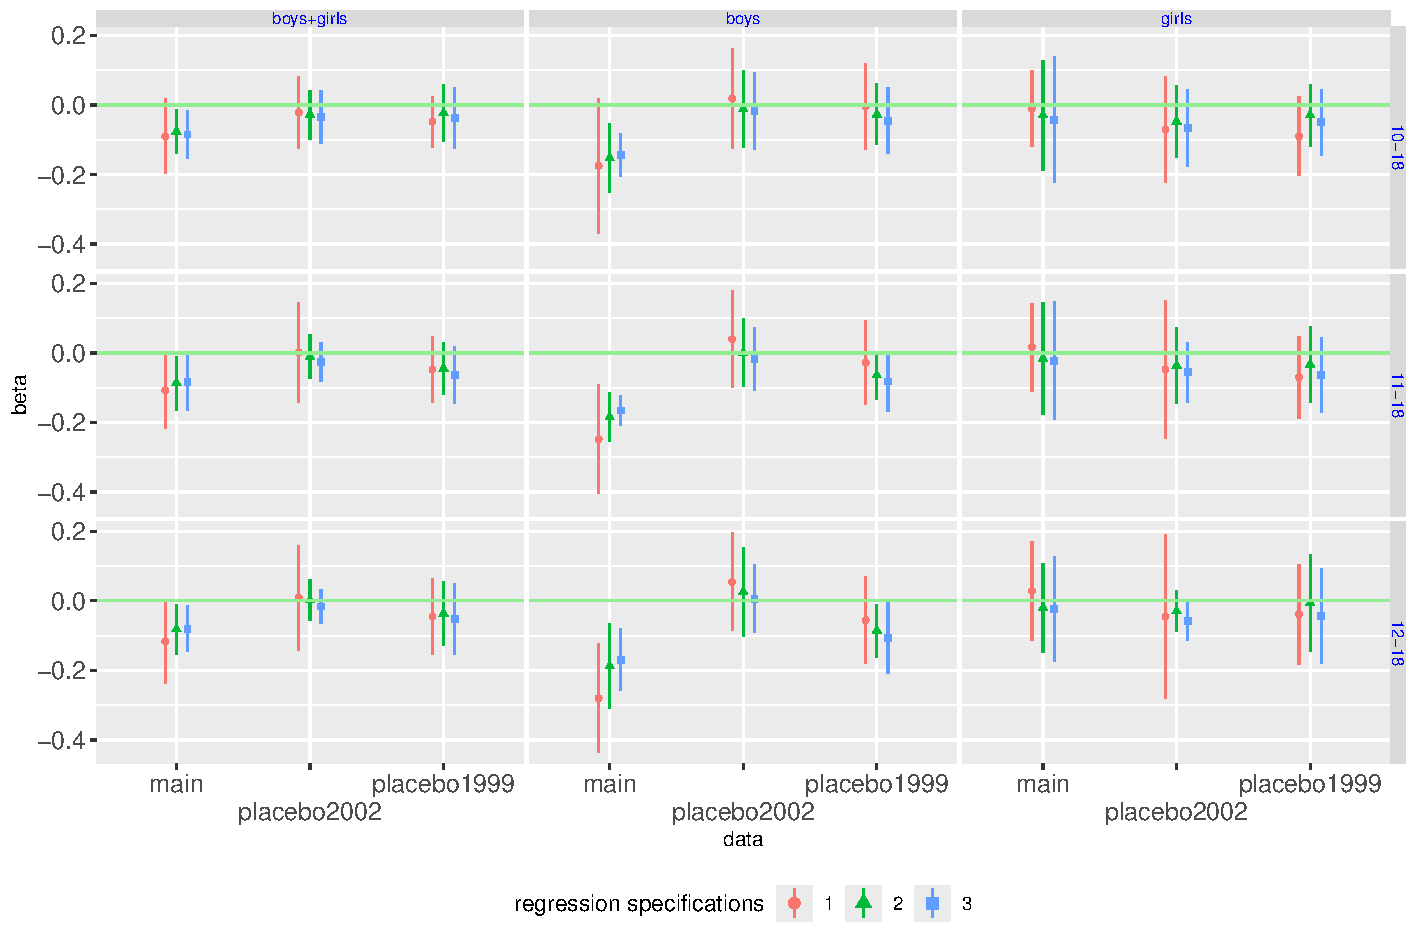
\includegraphics[height=.3\paperheight]{../draft/Figures/App_MainVsPlaceboPlotsByAgeLBByGender.pdf}\\
\renewcommand{\arraystretch}{1}
\hfil\begin{tabular}{>{\hfill\scriptsize}p{1cm}<{}>{\scriptsize}p{11cm}<{\hfill}}
Source: & Compiled from IFPRI data. \\[-1ex]
<<<<<<< HEAD
Notes:& 1. 10-18, 11-18, 12-18 indicate age range of each sample. The coefficients are dummies for agri-HH $\times$ year 2002.\\[-1ex]
=======
Notes:& 1. 10-18, 11-18, 12-18 indicate age range of each sample. The coefficients are for agricultural HH $\times$ year 2002.\\[-1ex]
>>>>>>> 41dec8f560b653fb2373d27136c157ebc2dfddbe
& 2. Specifications 1 - 3 correspond to the same specifications in \textsc{Table \ref{base10}}. \\[-1ex]
& 3. Error bars are 95\% confidence intervals using standard errors clustered at thana level with a Satterthwaite correction for small number of clusters.
\end{tabular}
%\end{minipage}
\end{figure}
<<<<<<< HEAD

\begin{figure}
%\hspace{-2em}\begin{minipage}[t]{13cm}
\hfil\textsc{\footnotesize Figure \refstepcounter{figure}\thefigure: Impacts by age group, 1999-2002, 6-17 years old in 1999\label{GenderAgeGroup2Impacts}}\\
\hfil 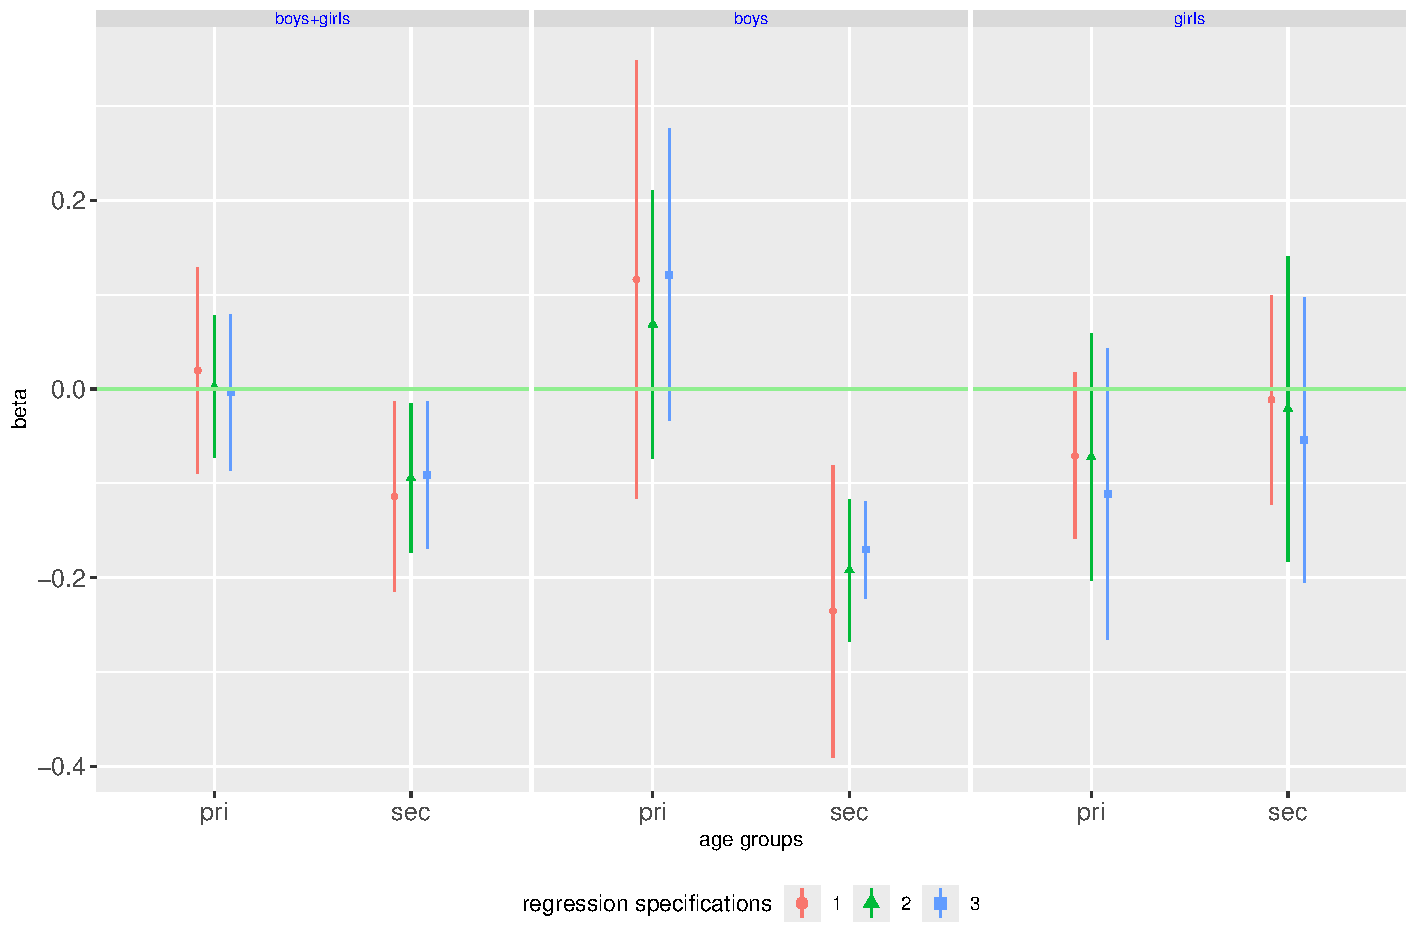
\includegraphics[height=.23\paperheight]{../draft/Figures/GenderAgeGroup2Impacts.pdf}\\
\renewcommand{\arraystretch}{1}
\hfil\begin{tabular}{>{\hfill\scriptsize}p{1cm}<{}>{\scriptsize}p{11cm}<{\hfill}}
Source: & Compiled from IFPRI data. \\[-1ex]
Notes:& 1. ``pri'' and ``sec'' mean enrolled in primary and secondary grades, aged 6-10 and 11-17 years in 1999, respectively. The coefficients are dummies for agri-HH $\times$ year 2002.\\[-1ex]
& 2. Specifications 1 - 3 correspond to the same specifications in \textsc{Table \ref{base10}}. \\[-1ex]
& 3. Error bars are 95\% confidence intervals using standard errors clustered at thana level with a Satterthwaite correction for small number of clusters.
\end{tabular}
%\end{minipage}
\end{figure}


=======
>>>>>>> 41dec8f560b653fb2373d27136c157ebc2dfddbe

\begin{figure}
%\hspace{-2em}\begin{minipage}[t]{13cm}
\hfil\textsc{\footnotesize Figure \refstepcounter{figure}\thefigure: Impacts by age group, 1999-2002, 6-17 years old in 1999\label{GenderAgeGroup2Impacts}}\\
\hfil 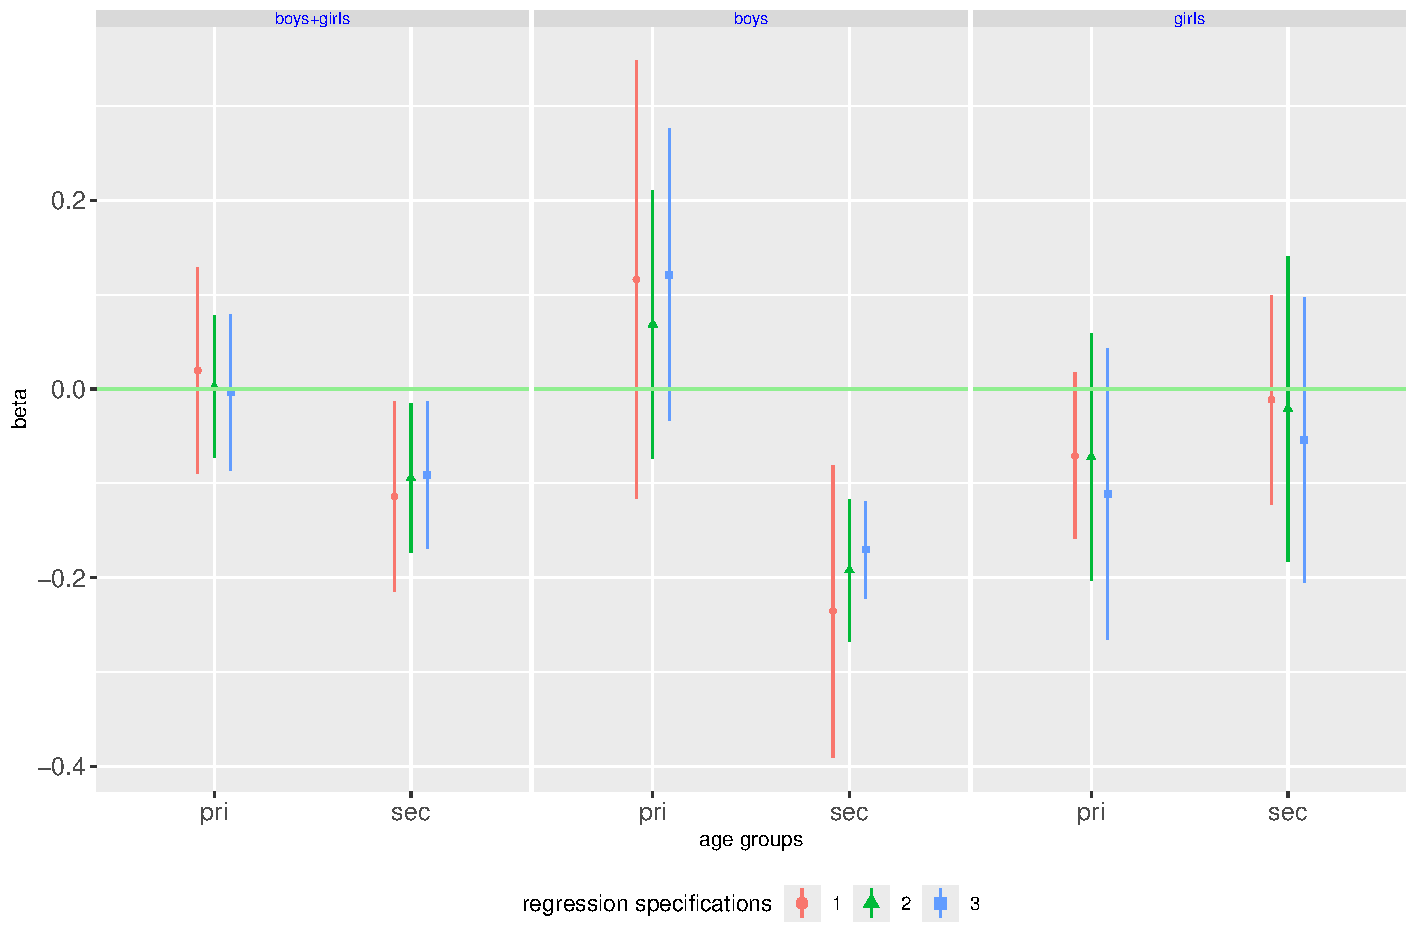
\includegraphics[height=.23\paperheight]{../draft/Figures/GenderAgeGroup2Impacts.pdf}\\
\renewcommand{\arraystretch}{1}
\hfil\begin{tabular}{>{\hfill\scriptsize}p{1cm}<{}>{\scriptsize}p{11cm}<{\hfill}}
Source: & Compiled from IFPRI data. \\[-1ex]
Notes:& 1. ``pri'' and ``sec'' mean enrolled in primary and secondary grades, aged 6-10 and 11-17 years in 1999, respectively. The coefficients are for agricultural HH $\times$ year 2002.\\[-1ex]
& 2. Specifications 1 - 3 correspond to the same specifications in \textsc{Table \ref{base10}}. \\[-1ex]
& 3. Error bars are 95\% confidence intervals using standard errors clustered at thana level with a Satterthwaite correction for small number of clusters.
\end{tabular}
%\end{minipage}
\end{figure}





\begin{table}\hfil\textsc{\footnotesize Table \refstepcounter{table}\thetable: Main results 1999-2002\label{zEm.1999.10.sameN}}\\\setlength{\tabcolsep}{.5pt}\renewcommand{\arraystretch}{.675}\hspace{-2em}\hfil\begin{tabular}{>{\scriptsize}p{3.25cm}<{\hfill}>{\hfil\scriptsize$}p{1.5cm}<{$}>{\hfil\scriptsize$}p{1.5cm}<{$}>{\hfil\scriptsize$}p{1.5cm}<{$}>{$}p{0.1cm}<{$}>{\hfil\scriptsize$}p{1.5cm}<{$}>{\hfil\scriptsize$}p{1.5cm}<{$}>{\hfil\scriptsize$}p{1.5cm}<{$}>{$}p{0.1cm}<{$}>{\hfil\scriptsize$}p{1.5cm}<{$}>{\hfil\scriptsize$}p{1.5cm}<{$}>{\hfil\scriptsize$}p{1.5cm}<{$}}
\hline
\makebox[3.25cm]{\scriptsize\hfil }&\multicolumn{3}{c}{\makebox[4.5cm]{\scriptsize \textsf{Boys+girls}}}&&\multicolumn{3}{c}{\makebox[4.5cm]{\scriptsize \textsf{Boys}}}&&\multicolumn{3}{c}{\makebox[3.1cm]{\scriptsize \textsf{Girls}}} \\[-.5ex]
\cline{2-4} \cline{6-8} \cline{10-12} \\[-1ex]
&\textsf{Spec 1} & \textsf{Spec 2} & \textsf{Spec 3}&&\textsf{Spec 1} & \textsf{Spec 2} & \textsf{Spec 3}&&\textsf{Spec 1} & \textsf{Spec 2} & \textsf{Spec 3}\\
&\multicolumn{11}{l}{}\\
A. AgHH: Head's reply & (1)&(2)&(3)&&(4)&(5)&(6)&&(7)&(8)&(9) \\
Agricultural HH * year 2002 & -0.0897^{*\phantom{**}} & -0.0761^{**\phantom{*}} & -0.0846^{**\phantom{*}} &  & -0.1749^{*\phantom{**}} & -0.1521^{***} & -0.1445^{***} &  & -0.0097^{\phantom{***}} & -0.0294^{\phantom{***}} & -0.0423^{\phantom{***}}\\[-.5ex]
\hspace{1em}  & (8.8) & (2.6) & (2.3) &  & (6.9) & (0.9) & (0.1) &  & (83.8) & (66.3) & (58.5)\\[-.5ex]
\hspace{1em}  & \mbox{\tiny [-0.197, 0.018]} & \mbox{\tiny [-0.140, -0.012]} & \mbox{\tiny [-0.153, -0.016]} &  & \mbox{\tiny [-0.368, 0.019]} & \mbox{\tiny [-0.251, -0.053]} & \mbox{\tiny [-0.206, -0.083]} &  & \mbox{\tiny [-0.119, 0.100]} & \mbox{\tiny [-0.187, 0.128]} & \mbox{\tiny [-0.223, 0.138]}\\
$\bar{R}^{2}$ & 0.0085 & 0.4446 & 0.4839 &  & 0.0328 & 0.3738 & 0.4199 &  & 0.0001 & 0.5928 & 0.6084\\
N: Agricultural HHs &   & 346 &   &  &   & 177 &   &  &   & 169 &  \\
N &   & 626 &   &  &   & 306 &   &  &   & 320 &  \\
Mean of control in 1999 &   & 0.7464 &   &  &   & 0.6512 &   &  &   & 0.8278 &  \\
Mean of treated in 1999 &   & 0.7312 &   &  &   & 0.6780 &   &  &   & 0.7870 &  \\
Mean of control in 2002 &   & 0.4893 &   &  &   & 0.4419 &   &  &   & 0.5298 &  \\
Mean of treated in 2002 &   & 0.3844 &   &  &   & 0.2938 &   &  &   & 0.4793 &  \\
&\multicolumn{11}{l}{}\\
B. AgHH: Income source & (10)&(11)&(12)&&(13)&(14)&(15)&&(16)&(17)&(18) \\
Agricultural HH * year 2002 & -0.0561^{\phantom{***}} & -0.0661^{*\phantom{**}} & -0.0899^{**\phantom{*}} &  & -0.1290^{\phantom{***}} & -0.1550^{**\phantom{*}} & -0.1441^{***} &  & \phantom{-}0.0105^{\phantom{***}} & -0.0268^{\phantom{***}} & -0.0503^{\phantom{***}}\\[-.5ex]
\hspace{1em}  & (27.5) & (6.0) & (1.1) &  & (12.4) & (1.6) & (0.4) &  & (88.6) & (71.4) & (53.2)\\[-.5ex]
\hspace{1em}  & \mbox{\tiny [-0.169, 0.057]} & \mbox{\tiny [-0.136, 0.004]} & \mbox{\tiny [-0.151, -0.029]} &  & \mbox{\tiny [-0.305, 0.047]} & \mbox{\tiny [-0.270, -0.040]} & \mbox{\tiny [-0.221, -0.067]} &  & \mbox{\tiny [-0.159, 0.180]} & \mbox{\tiny [-0.196, 0.143]} & \mbox{\tiny [-0.237, 0.136]}\\
$\bar{R}^{2}$ & 0.0033 & 0.4432 & 0.4868 &  & 0.0173 & 0.3734 & 0.4186 &  & 0.0001 & 0.5926 & 0.6124\\
N: Agricultural HHs &   & 360 &   &  &   & 189 &   &  &   & 171 &  \\
N &   & 626 &   &  &   & 306 &   &  &   & 320 &  \\
Mean of control in 1999 &   & 0.7744 &   &  &   & 0.7094 &   &  &   & 0.8255 &  \\
Mean of treated in 1999 &   & 0.7111 &   &  &   & 0.6402 &   &  &   & 0.7895 &  \\
Mean of control in 2002 &   & 0.5000 &   &  &   & 0.4786 &   &  &   & 0.5168 &  \\
Mean of treated in 2002 &   & 0.3806 &   &  &   & 0.2804 &   &  &   & 0.4912 &  \\
&\multicolumn{11}{l}{}\\
C. AgHH: Occupation & (19)&(20)&(21)&&(22)&(23)&(24)&&(25)&(26)&(27) \\
Agricultural HH * year 2002 & -0.0111^{\phantom{***}} & -0.0402^{\phantom{***}} & -0.0535^{**\phantom{*}} &  & -0.0556^{\phantom{***}} & -0.1194^{**\phantom{*}} & -0.1024^{**\phantom{*}} &  & \phantom{-}0.0313^{\phantom{***}} & -0.0024^{\phantom{***}} & -0.0172^{\phantom{***}}\\[-.5ex]
\hspace{1em}  & (79.3) & (12.4) & (2.7) &  & (40.9) & (3.7) & (4.7) &  & (67.4) & (96.9) & (80.3)\\[-.5ex]
\hspace{1em}  & \mbox{\tiny [-0.108, 0.085]} & \mbox{\tiny [-0.095, 0.014]} & \mbox{\tiny [-0.099, -0.008]} &  & \mbox{\tiny [-0.206, 0.095]} & \mbox{\tiny [-0.229, -0.010]} & \mbox{\tiny [-0.203, -0.002]} &  & \mbox{\tiny [-0.140, 0.202]} & \mbox{\tiny [-0.148, 0.144]} & \mbox{\tiny [-0.178, 0.144]}\\
$\bar{R}^{2}$ & 0.0001 & 0.4407 & 0.4790 &  & 0.0033 & 0.3655 & 0.4043 &  & 0.0010 & 0.5920 & 0.6064\\
N: Agricultural HHs &   & 340 &   &  &   & 180 &   &  &   & 160 &  \\
N &   & 626 &   &  &   & 306 &   &  &   & 320 &  \\
Mean of control in 1999 &   & 0.7867 &   &  &   & 0.7222 &   &  &   & 0.8375 &  \\
Mean of treated in 1999 &   & 0.6971 &   &  &   & 0.6278 &   &  &   & 0.7750 &  \\
Mean of control in 2002 &   & 0.4860 &   &  &   & 0.4444 &   &  &   & 0.5188 &  \\
Mean of treated in 2002 &   & 0.3853 &   &  &   & 0.2944 &   &  &   & 0.4875 &  \\
&\multicolumn{11}{l}{}\\
D. AgHH: Combined & (28)&(29)&(30)&&(31)&(32)&(33)&&(34)&(35)&(36) \\
Agricultural HH * year 2002 & -0.0419^{\phantom{***}} & -0.0571^{*\phantom{**}} & -0.0770^{**\phantom{*}} &  & -0.0975^{\phantom{***}} & -0.1287^{**\phantom{*}} & -0.1202^{**\phantom{*}} &  & \phantom{-}0.0088^{\phantom{***}} & -0.0242^{\phantom{***}} & -0.0472^{\phantom{***}}\\[-.5ex]
\hspace{1em}  & (38.8) & (7.7) & (3.2) &  & (24.2) & (3.5) & (1.8) &  & (90.5) & (74.6) & (56.7)\\[-.5ex]
\hspace{1em}  & \mbox{\tiny [-0.151, 0.067]} & \mbox{\tiny [-0.123, 0.008]} & \mbox{\tiny [-0.144, -0.009]} &  & \mbox{\tiny [-0.280, 0.085]} & \mbox{\tiny [-0.245, -0.012]} & \mbox{\tiny [-0.211, -0.029]} &  & \mbox{\tiny [-0.163, 0.180]} & \mbox{\tiny [-0.200, 0.152]} & \mbox{\tiny [-0.240, 0.145]}\\
$\bar{R}^{2}$ & 0.0018 & 0.4421 & 0.4839 &  & 0.0096 & 0.3662 & 0.4148 &  & 0.0001 & 0.5925 & 0.6104\\
N: Agricultural HHs &   & 384 &   &  &   & 197 &   &  &   & 187 &  \\
N &   & 626 &   &  &   & 306 &   &  &   & 320 &  \\
Mean of control in 1999 &   & 0.7769 &   &  &   & 0.7156 &   &  &   & 0.8271 &  \\
Mean of treated in 1999 &   & 0.7135 &   &  &   & 0.6396 &   &  &   & 0.7914 &  \\
Mean of control in 2002 &   & 0.4959 &   &  &   & 0.4679 &   &  &   & 0.5188 &  \\
Mean of treated in 2002 &   & 0.3906 &   &  &   & 0.2944 &   &  &   & 0.4920 &  \\
\hline
\end{tabular}
\\\renewcommand{\arraystretch}{1}\hfil\begin{tabular}{>{\hfill\scriptsize}p{1cm}<{}>{\scriptsize}p{12cm}<{\hfill}} Source:& Compiled from IFPRI data. \\[-1ex] Notes:&   \textsf{Agricultural HH * year 2002} is an interaction term of agricultural household dummy and year 2002 dummy. All interaction terms are demeaned. Panels A. - D. give estimates under different agricultural household definitions. A: income source base, B: Head's reply base, C: Occupation base, D: All combined (with ``or'' operations). For each panel, first columns are raw DID. Second columns add time-varying thana level characteristics (yield, mean rainfall, mean high temperature, mean low temperature), individual level characteristics (age squared, recipient of a poverty program), and \textsf{Thana trends} that are interactions of year 2002 dummy with Thana fixed effects. Third columns add interactions of year 2002 dummy and individual level characterstics (sex of individual, household head's and spouse's education, number of older male/female siblings, per member land holding, per member non land asset holding, piped water access, structured toilet access) $\bfx_{i}r_{t}$, and triple interactions of year 2002 dummy, individual characteristics, and agricultural household dummy $\bfx_{i}r_{t}D_{i}$. Rows of $\underline{\phantom{mm}}*x$ show estimates of the triple interaction term of $x_{i}$, or $x_{i}r_{t}D_{i}$. Parental education variables are strongly collinear with agricultural household dummy and are used only in year 2002 interaction terms to avoid multicollinearity., \\   \end{tabular} \end{table}

\begin{table}\hfil\textsc{\footnotesize Table \refstepcounter{table}\thetable: Main results 1999-2002\label{zEm.1999.10.sameN}}\\\setlength{\tabcolsep}{.5pt}\renewcommand{\arraystretch}{.675}\hspace{-2em}\hfil\begin{tabular}{>{\scriptsize}p{3.25cm}<{\hfill}>{\hfil\scriptsize$}p{1.5cm}<{$}>{\hfil\scriptsize$}p{1.5cm}<{$}>{\hfil\scriptsize$}p{1.5cm}<{$}>{$}p{0.1cm}<{$}>{\hfil\scriptsize$}p{1.5cm}<{$}>{\hfil\scriptsize$}p{1.5cm}<{$}>{\hfil\scriptsize$}p{1.5cm}<{$}>{$}p{0.1cm}<{$}>{\hfil\scriptsize$}p{1.5cm}<{$}>{\hfil\scriptsize$}p{1.5cm}<{$}>{\hfil\scriptsize$}p{1.5cm}<{$}}
\hline
\makebox[3.25cm]{\scriptsize\hfil }&\multicolumn{3}{c}{\makebox[4.5cm]{\scriptsize \textsf{Boys+girls}}}&&\multicolumn{3}{c}{\makebox[4.5cm]{\scriptsize \textsf{Boys}}}&&\multicolumn{3}{c}{\makebox[3.1cm]{\scriptsize \textsf{Girls}}} \\[-.5ex]
\cline{2-4} \cline{6-8} \cline{10-12} \\[-1ex]
&\textsf{Spec 1} & \textsf{Spec 2} & \textsf{Spec 3}&&\textsf{Spec 1} & \textsf{Spec 2} & \textsf{Spec 3}&&\textsf{Spec 1} & \textsf{Spec 2} & \textsf{Spec 3}\\
&\multicolumn{11}{l}{}\\
A. AgHH: Head's reply & (1)&(2)&(3)&&(4)&(5)&(6)&&(7)&(8)&(9) \\
Agricultural HH * year 2002 & -0.0897^{*\phantom{**}} & -0.0761^{**\phantom{*}} & -0.0846^{**\phantom{*}} &  & -0.1749^{*\phantom{**}} & -0.1521^{***} & -0.1445^{***} &  & -0.0097^{\phantom{***}} & -0.0294^{\phantom{***}} & -0.0423^{\phantom{***}}\\[-.5ex]
\hspace{1em}  & (8.8) & (2.6) & (2.3) &  & (6.9) & (0.9) & (0.1) &  & (83.8) & (66.3) & (58.5)\\[-.5ex]
\hspace{1em}  & \mbox{\tiny [-0.197, 0.018]} & \mbox{\tiny [-0.140, -0.012]} & \mbox{\tiny [-0.153, -0.016]} &  & \mbox{\tiny [-0.368, 0.019]} & \mbox{\tiny [-0.251, -0.053]} & \mbox{\tiny [-0.206, -0.083]} &  & \mbox{\tiny [-0.119, 0.100]} & \mbox{\tiny [-0.187, 0.128]} & \mbox{\tiny [-0.223, 0.138]}\\
\underline{\phantom{mm}} * Older sisters &  &  & -0.0281^{\phantom{***}} &  &  &  & -0.0817^{\phantom{***}} &  &  &  & \phantom{-}0.0088^{\phantom{***}}\\[-.5ex]
\hspace{1em}  &  &  & (43.0) &  &  &  & (10.7) &  &  &  & (93.1)\\[-.5ex]
\hspace{1em}  &  &  & \mbox{\tiny [-0.113, 0.057]} &  &  &  & \mbox{\tiny [-0.189, 0.026]} &  &  &  & \mbox{\tiny [-0.248, 0.266]}\\
\underline{\phantom{mm}} * Older brothers &  &  & -0.0573^{\phantom{***}} &  &  &  & -0.0057^{\phantom{***}} &  &  &  & -0.0721^{\phantom{***}}\\[-.5ex]
\hspace{1em}  &  &  & (28.8) &  &  &  & (91.1) &  &  &  & (22.2)\\[-.5ex]
\hspace{1em}  &  &  & \mbox{\tiny [-0.179, 0.064]} &  &  &  & \mbox{\tiny [-0.128, 0.117]} &  &  &  & \mbox{\tiny [-0.204, 0.060]}\\
$\bar{R}^{2}$ & 0.0085 & 0.4446 & 0.4839 &  & 0.0328 & 0.3738 & 0.4199 &  & 0.0001 & 0.5928 & 0.6084\\
N: Agricultural HHs &   & 346 &   &  &   & 177 &   &  &   & 169 &  \\
N &   & 626 &   &  &   & 306 &   &  &   & 320 &  \\
Mean of control in 1999 &   & 0.7464 &   &  &   & 0.6512 &   &  &   & 0.8278 &  \\
Mean of treated in 1999 &   & 0.7312 &   &  &   & 0.6780 &   &  &   & 0.7870 &  \\
Mean of control in 2002 &   & 0.4893 &   &  &   & 0.4419 &   &  &   & 0.5298 &  \\
Mean of treated in 2002 &   & 0.3844 &   &  &   & 0.2938 &   &  &   & 0.4793 &  \\
&\multicolumn{11}{l}{}\\
B. AgHH: Income source & (10)&(11)&(12)&&(13)&(14)&(15)&&(16)&(17)&(18) \\
Agricultural HH * year 2002 & -0.0561^{\phantom{***}} & -0.0661^{*\phantom{**}} & -0.0899^{**\phantom{*}} &  & -0.1290^{\phantom{***}} & -0.1550^{**\phantom{*}} & -0.1441^{***} &  & \phantom{-}0.0105^{\phantom{***}} & -0.0268^{\phantom{***}} & -0.0503^{\phantom{***}}\\[-.5ex]
\hspace{1em}  & (27.5) & (6.0) & (1.1) &  & (12.4) & (1.6) & (0.4) &  & (88.6) & (71.4) & (53.2)\\[-.5ex]
\hspace{1em}  & \mbox{\tiny [-0.169, 0.057]} & \mbox{\tiny [-0.136, 0.004]} & \mbox{\tiny [-0.151, -0.029]} &  & \mbox{\tiny [-0.305, 0.047]} & \mbox{\tiny [-0.270, -0.040]} & \mbox{\tiny [-0.221, -0.067]} &  & \mbox{\tiny [-0.159, 0.180]} & \mbox{\tiny [-0.196, 0.143]} & \mbox{\tiny [-0.237, 0.136]}\\
\underline{\phantom{mm}} * Older sisters &  &  & -0.0228^{\phantom{***}} &  &  &  & -0.0840^{*\phantom{**}} &  &  &  & \phantom{-}0.0080^{\phantom{***}}\\[-.5ex]
\hspace{1em}  &  &  & (54.4) &  &  &  & (8.4) &  &  &  & (93.6)\\[-.5ex]
\hspace{1em}  &  &  & \mbox{\tiny [-0.114, 0.068]} &  &  &  & \mbox{\tiny [-0.185, 0.017]} &  &  &  & \mbox{\tiny [-0.241, 0.257]}\\
\underline{\phantom{mm}} * Older brothers &  &  & -0.0904^{\phantom{***}} &  &  &  & -0.0280^{\phantom{***}} &  &  &  & -0.1040^{**\phantom{*}}\\[-.5ex]
\hspace{1em}  &  &  & (10.8) &  &  &  & (66.6) &  &  &  & (2.6)\\[-.5ex]
\hspace{1em}  &  &  & \mbox{\tiny [-0.209, 0.028]} &  &  &  & \mbox{\tiny [-0.190, 0.134]} &  &  &  & \mbox{\tiny [-0.189, -0.019]}\\
$\bar{R}^{2}$ & 0.0033 & 0.4432 & 0.4868 &  & 0.0173 & 0.3734 & 0.4186 &  & 0.0001 & 0.5926 & 0.6124\\
N: Agricultural HHs &   & 360 &   &  &   & 189 &   &  &   & 171 &  \\
N &   & 626 &   &  &   & 306 &   &  &   & 320 &  \\
Mean of control in 1999 &   & 0.7744 &   &  &   & 0.7094 &   &  &   & 0.8255 &  \\
Mean of treated in 1999 &   & 0.7111 &   &  &   & 0.6402 &   &  &   & 0.7895 &  \\
Mean of control in 2002 &   & 0.5000 &   &  &   & 0.4786 &   &  &   & 0.5168 &  \\
Mean of treated in 2002 &   & 0.3806 &   &  &   & 0.2804 &   &  &   & 0.4912 &  \\
\hline
\end{tabular}
\\\renewcommand{\arraystretch}{1}\end{table}, \addtocounter{table}{-1}, \begin{table}\hfil\textsc{\footnotesize Table \refstepcounter{table}\thetable: Main results 1999-2002 (continued)\label{zEm.1999.10.sameN}}\\\setlength{\tabcolsep}{.5pt}\renewcommand{\arraystretch}{.675}\hspace{-3cm}\hfil\begin{tikzpicture}\node (tbl) {\begin{tabular}{>{\scriptsize}p{3.25cm}<{\hfill}>{\hfil\scriptsize$}p{1.5cm}<{$}>{\hfil\scriptsize$}p{1.5cm}<{$}>{\hfil\scriptsize$}p{1.5cm}<{$}>{$}p{0.1cm}<{$}>{\hfil\scriptsize$}p{1.5cm}<{$}>{\hfil\scriptsize$}p{1.5cm}<{$}>{\hfil\scriptsize$}p{1.5cm}<{$}>{$}p{0.1cm}<{$}>{\hfil\scriptsize$}p{1.5cm}<{$}>{\hfil\scriptsize$}p{1.5cm}<{$}>{\hfil\scriptsize$}p{1.5cm}<{$}}
\hline
\makebox[3.25cm]{\scriptsize\hfil }&\multicolumn{3}{c}{\makebox[4.5cm]{\scriptsize \textsf{Boys+girls}}}&&\multicolumn{3}{c}{\makebox[4.5cm]{\scriptsize \textsf{Boys}}}&&\multicolumn{3}{c}{\makebox[3.1cm]{\scriptsize \textsf{Girls}}} \\[-.5ex]
\cline{2-4} \cline{6-8} \cline{10-12} \\[-1ex]
&\multicolumn{11}{l}{}\\
C. AgHH: Occupation & (19)&(20)&(21)&&(22)&(23)&(24)&&(25)&(26)&(27) \\
Agricultural HH * year 2002 & -0.0111^{\phantom{***}} & -0.0402^{\phantom{***}} & -0.0535^{**\phantom{*}} &  & -0.0556^{\phantom{***}} & -0.1194^{**\phantom{*}} & -0.1024^{**\phantom{*}} &  & \phantom{-}0.0313^{\phantom{***}} & -0.0024^{\phantom{***}} & -0.0172^{\phantom{***}}\\[-.5ex]
\hspace{1em}  & (79.3) & (12.4) & (2.7) &  & (40.9) & (3.7) & (4.7) &  & (67.4) & (96.9) & (80.3)\\[-.5ex]
\hspace{1em}  & \mbox{\tiny [-0.108, 0.085]} & \mbox{\tiny [-0.095, 0.014]} & \mbox{\tiny [-0.099, -0.008]} &  & \mbox{\tiny [-0.206, 0.095]} & \mbox{\tiny [-0.229, -0.010]} & \mbox{\tiny [-0.203, -0.002]} &  & \mbox{\tiny [-0.140, 0.202]} & \mbox{\tiny [-0.148, 0.144]} & \mbox{\tiny [-0.178, 0.144]}\\
\underline{\phantom{mm}} * Older sisters &  &  & -0.0159^{\phantom{***}} &  &  &  & -0.0758^{\phantom{***}} &  &  &  & \phantom{-}0.0265^{\phantom{***}}\\[-.5ex]
\hspace{1em}  &  &  & (63.9) &  &  &  & (15.2) &  &  &  & (74.9)\\[-.5ex]
\hspace{1em}  &  &  & \mbox{\tiny [-0.098, 0.067]} &  &  &  & \mbox{\tiny [-0.192, 0.041]} &  &  &  & \mbox{\tiny [-0.178, 0.230]}\\
\underline{\phantom{mm}} * Older brothers &  &  & -0.0672^{\phantom{***}} &  &  &  & -0.0312^{\phantom{***}} &  &  &  & -0.0563^{\phantom{***}}\\[-.5ex]
\hspace{1em}  &  &  & (24.0) &  &  &  & (61.5) &  &  &  & (36.0)\\[-.5ex]
\hspace{1em}  &  &  & \mbox{\tiny [-0.195, 0.060]} &  &  &  & \mbox{\tiny [-0.182, 0.120]} &  &  &  & \mbox{\tiny [-0.198, 0.086]}\\
$\bar{R}^{2}$ & 0.0001 & 0.4407 & 0.4790 &  & 0.0033 & 0.3655 & 0.4043 &  & 0.0010 & 0.5920 & 0.6064\\
N: Agricultural HHs &   & 340 &   &  &   & 180 &   &  &   & 160 &  \\
N &   & 626 &   &  &   & 306 &   &  &   & 320 &  \\
Mean of control in 1999 &   & 0.7867 &   &  &   & 0.7222 &   &  &   & 0.8375 &  \\
Mean of treated in 1999 &   & 0.6971 &   &  &   & 0.6278 &   &  &   & 0.7750 &  \\
Mean of control in 2002 &   & 0.4860 &   &  &   & 0.4444 &   &  &   & 0.5188 &  \\
Mean of treated in 2002 &   & 0.3853 &   &  &   & 0.2944 &   &  &   & 0.4875 &  \\
&\multicolumn{11}{l}{}\\
D. AgHH: Combined & (28)&(29)&(30)&&(31)&(32)&(33)&&(34)&(35)&(36) \\
Agricultural HH * year 2002 & -0.0419^{\phantom{***}} & -0.0571^{*\phantom{**}} & -0.0770^{**\phantom{*}} &  & -0.0975^{\phantom{***}} & -0.1287^{**\phantom{*}} & -0.1202^{**\phantom{*}} &  & \phantom{-}0.0088^{\phantom{***}} & -0.0242^{\phantom{***}} & -0.0472^{\phantom{***}}\\[-.5ex]
\hspace{1em}  & (38.8) & (7.7) & (3.2) &  & (24.2) & (3.5) & (1.8) &  & (90.5) & (74.6) & (56.7)\\[-.5ex]
\hspace{1em}  & \mbox{\tiny [-0.151, 0.067]} & \mbox{\tiny [-0.123, 0.008]} & \mbox{\tiny [-0.144, -0.009]} &  & \mbox{\tiny [-0.280, 0.085]} & \mbox{\tiny [-0.245, -0.012]} & \mbox{\tiny [-0.211, -0.029]} &  & \mbox{\tiny [-0.163, 0.180]} & \mbox{\tiny [-0.200, 0.152]} & \mbox{\tiny [-0.240, 0.145]}\\
\underline{\phantom{mm}} * Older sisters &  &  & -0.0286^{\phantom{***}} &  &  &  & -0.1106^{**\phantom{*}} &  &  &  & \phantom{-}0.0289^{\phantom{***}}\\[-.5ex]
\hspace{1em}  &  &  & (44.4) &  &  &  & (3.7) &  &  &  & (77.1)\\[-.5ex]
\hspace{1em}  &  &  & \mbox{\tiny [-0.119, 0.062]} &  &  &  & \mbox{\tiny [-0.210, -0.011]} &  &  &  & \mbox{\tiny [-0.219, 0.277]}\\
\underline{\phantom{mm}} * Older brothers &  &  & -0.0964^{\phantom{***}} &  &  &  & -0.0521^{\phantom{***}} &  &  &  & -0.0911^{\phantom{***}}\\[-.5ex]
\hspace{1em}  &  &  & (11.9) &  &  &  & (41.9) &  &  &  & (15.1)\\[-.5ex]
\hspace{1em}  &  &  & \mbox{\tiny [-0.229, 0.036]} &  &  &  & \mbox{\tiny [-0.209, 0.105]} &  &  &  & \mbox{\tiny [-0.231, 0.048]}\\
$\bar{R}^{2}$ & 0.0018 & 0.4421 & 0.4839 &  & 0.0096 & 0.3662 & 0.4148 &  & 0.0001 & 0.5925 & 0.6104\\
N: Agricultural HHs &   & 384 &   &  &   & 197 &   &  &   & 187 &  \\
N &   & 626 &   &  &   & 306 &   &  &   & 320 &  \\
Mean of control in 1999 &   & 0.7769 &   &  &   & 0.7156 &   &  &   & 0.8271 &  \\
Mean of treated in 1999 &   & 0.7135 &   &  &   & 0.6396 &   &  &   & 0.7914 &  \\
Mean of control in 2002 &   & 0.4959 &   &  &   & 0.4679 &   &  &   & 0.5188 &  \\
Mean of treated in 2002 &   & 0.3906 &   &  &   & 0.2944 &   &  &   & 0.4920 &  \\
\hline
\end{tabular}
};\input{c:/data/ramadan/save/tablecolortemplate.tex}\end{tikzpicture}\\\renewcommand{\arraystretch}{1}\hfil\begin{tabular}{>{\hfill\scriptsize}p{1cm}<{}>{\scriptsize}p{12cm}<{\hfill}} Source:& Compiled from IFPRI data. \\[-1ex] Notes:&   \textsf{Agricultural HH * year 2002} is an interaction term of agricultural household dummy and year 2002 dummy. All interaction terms are demeaned. Panels A. - D. give estimates under different agricultural household definitions. A: income source base, B: Head's reply base, C: Occupation base, D: All combined (with ``or'' operations). For each panel, first columns are raw DID. Second columns add time-varying thana level characteristics (yield, mean rainfall, mean high temperature, mean low temperature), individual level characteristics (age squared, recipient of a poverty program), and \textsf{Thana trends} that are interactions of year 2002 dummy with Thana fixed effects. Third columns add interactions of year 2002 dummy and individual level characterstics (sex of individual, household head's and spouse's education, number of older male/female siblings, per member land holding, per member non land asset holding, piped water access, structured toilet access) $\bfx_{i}r_{t}$, and triple interactions of year 2002 dummy, individual characteristics, and agricultural household dummy $\bfx_{i}r_{t}D_{i}$. Rows of $\underline{\phantom{mm}}*x$ show estimates of the triple interaction term of $x_{i}$, or $x_{i}r_{t}D_{i}$. Parental education variables are strongly collinear with agricultural household dummy and are used only in year 2002 interaction terms to avoid multicollinearity., \\   \end{tabular} \end{table}



\clearpage
\subsection{Robustness}

\subsubsection{Placebo}


<<<<<<< HEAD
=======

>>>>>>> 41dec8f560b653fb2373d27136c157ebc2dfddbe
\begin{figure}
%\hspace{-2em}\begin{minipage}[t]{13cm}
\hfil\textsc{\footnotesize Figure \refstepcounter{figure}\thefigure: Impacts by main/placebo by gender and by agricutural household definition\label{App_MainVsPlaceboPlotsByAgdefByGender}}\\
\hfil 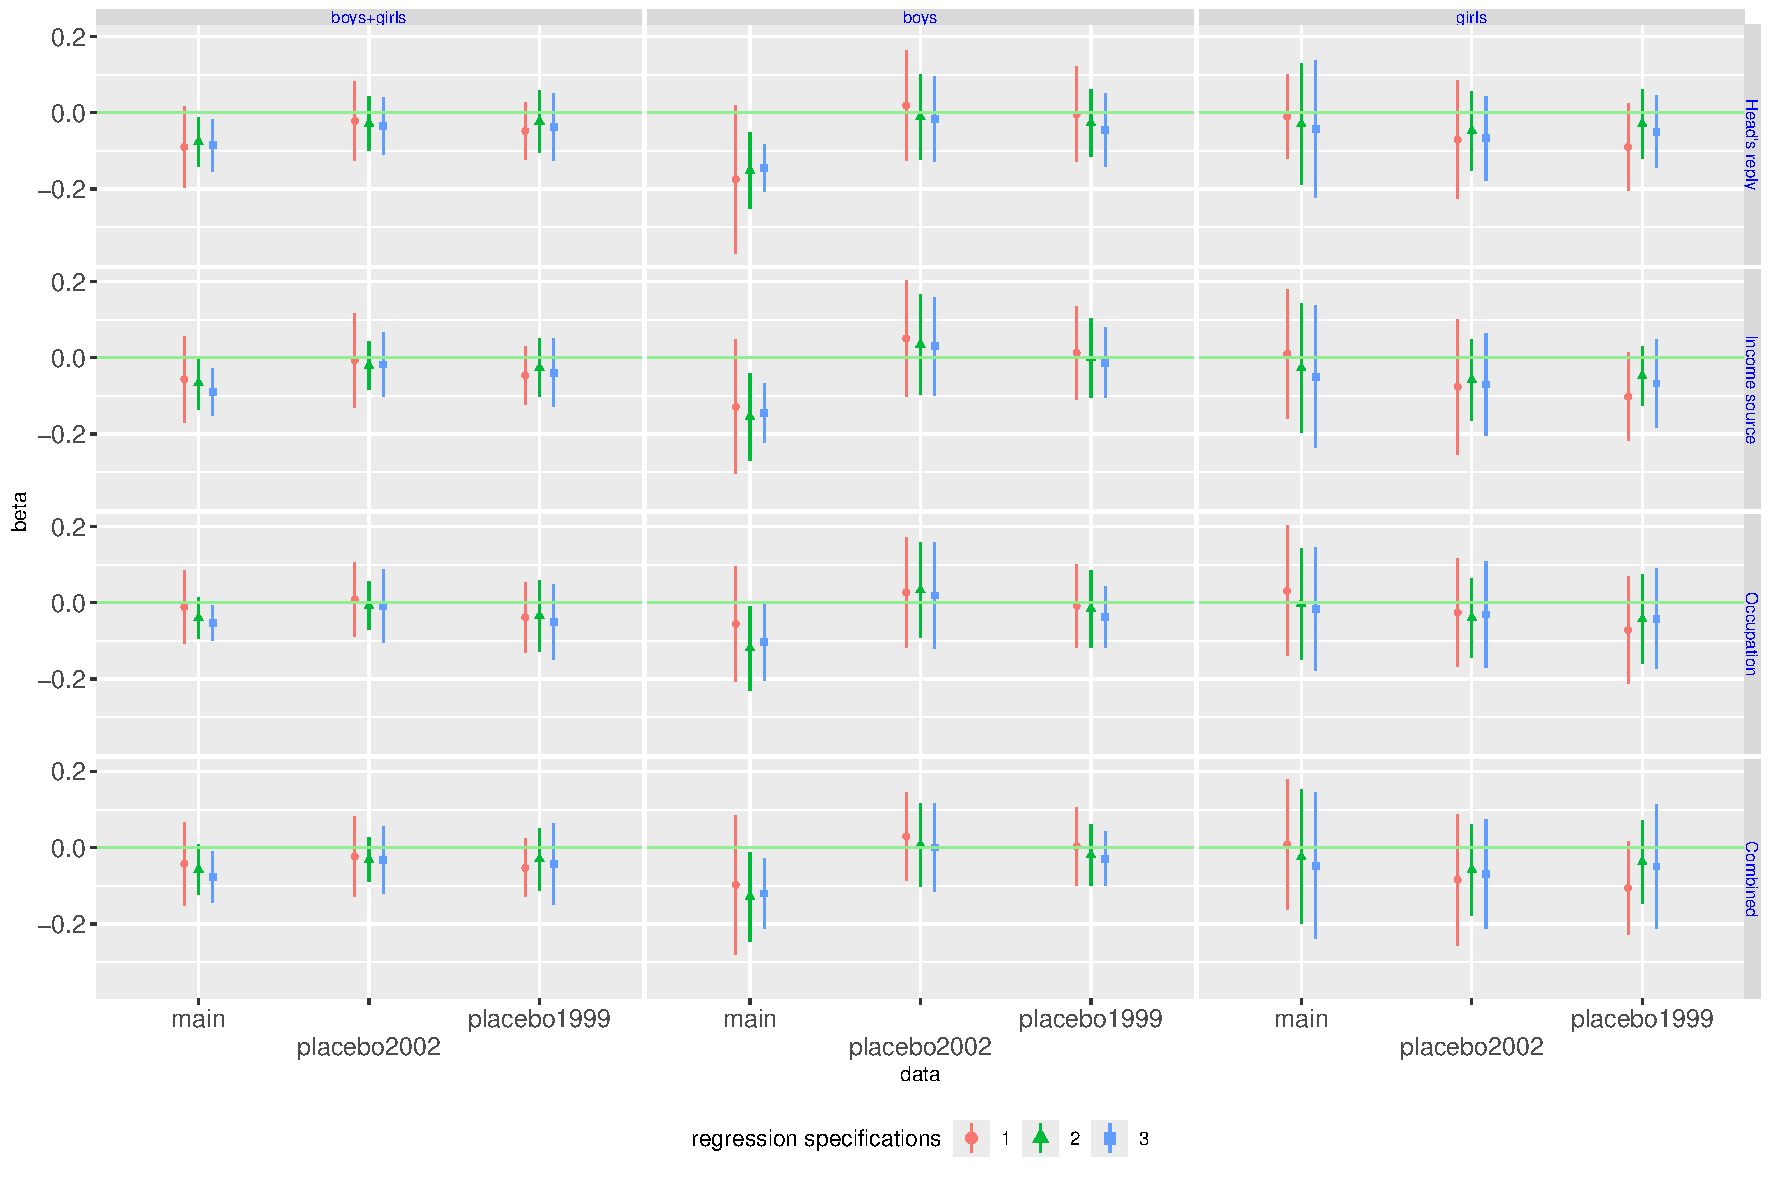
\includegraphics[height=.3\paperheight]{../draft/Figures/App_MainVsPlaceboPlotsByAgdefByGender.pdf}\\
\renewcommand{\arraystretch}{1}
\hfil\begin{tabular}{>{\hfill\scriptsize}p{1cm}<{}>{\scriptsize}p{11cm}<{\hfill}}
Source: & Compiled from IFPRI data. \\[-1ex]
<<<<<<< HEAD
Notes:& 1. ``pri'' and ``sec'' mean enrolled in primary and secondary grades, aged 6-10 and 11-17 years in 1999, respectively. The coefficients are dummies for agri-HH $\times$ year 2002.\\[-1ex]
=======
Notes:& 1. Each row shows the estimates under different agricultural household definitions. A: income source base, B: Head's reply base, C: Occupation base, D: All combined (with ``or'' operations). Each column shows estimates using gender subsamples and full sample. The coefficients are for agricultural HH $\times$ year 2002 for main data and agricultural HH $\times$ year 2006 for placebo 2002 and placebo 1999 data.\\[-1ex]
>>>>>>> 41dec8f560b653fb2373d27136c157ebc2dfddbe
& 2. Specifications 1 - 3 correspond to the same specifications in \textsc{Table \ref{base10}}. \\[-1ex]
& 3. Error bars are 95\% confidence intervals using standard errors clustered at thana level with a Satterthwaite correction for small number of clusters.
\end{tabular}
%\end{minipage}
\end{figure}



<<<<<<< HEAD
\begin{table}\hfil\textsc{\footnotesize Table \refstepcounter{table}\thetable: Placebo estimation 2002-2006, 1999 and 2002 cohorts\label{zEm.1999.10.sameN}}\\\setlength{\tabcolsep}{.5pt}\renewcommand{\arraystretch}{.675}\hspace{-2em}\hfil<<<<<<< HEAD
\begin{tabular}{>{\scriptsize}p{3cm}<{\hfill}>{\hfil\scriptsize$}p{1.3cm}<{$}>{\hfil\scriptsize$}p{1.3cm}<{$}>{\hfil\scriptsize$}p{1.3cm}<{$}>{$}p{0.1cm}<{$}>{\hfil\scriptsize$}p{1.3cm}<{$}>{\hfil\scriptsize$}p{1.3cm}<{$}>{\hfil\scriptsize$}p{1.3cm}<{$}>{$}p{0.1cm}<{$}>{\hfil\scriptsize$}p{1.3cm}<{$}>{\hfil\scriptsize$}p{1.3cm}<{$}>{\hfil\scriptsize$}p{1.3cm}<{$}}
\hline
\makebox[3cm]{\scriptsize\hfil }&\multicolumn{3}{c}{\makebox[3.9cm]{\scriptsize \textsf{Boys+Girls}}}&&\multicolumn{3}{c}{\makebox[3.9cm]{\scriptsize \textsf{Boys}}}&&\multicolumn{3}{c}{\makebox[2.7cm]{\scriptsize \textsf{Girls}}} \\[-.5ex]
\cline{2-4} \cline{6-8} \cline{10-12} \\[-1ex]
&\multicolumn{11}{c}{\scriptsize A. 2002 cohort}\\
\makebox[3cm]{rnm} & \makebox[1.3cm]{(1)} & \makebox[1.3cm]{(2)} & \makebox[1.3cm]{(3)} & \makebox[0.1cm]{} & \makebox[1.3cm]{(1)} & \makebox[1.3cm]{(2)} & \makebox[1.3cm]{(3)} & \makebox[0.1cm]{} & \makebox[1.3cm]{(1)} & \makebox[1.3cm]{(2)} & \makebox[1.3cm]{(3)}\\
Agricultural HH * year 2006 & -0.048^{\phantom{***}} & -0.023^{\phantom{***}} & -0.037^{\phantom{***}} &  & -0.004^{\phantom{***}} & -0.027^{\phantom{***}} & -0.045^{\phantom{***}} &  & -0.090^{\phantom{***}} & -0.029^{\phantom{***}} & -0.049^{\phantom{***}}\\[-1ex]
se$_{agHH.yr3}$ & (0.031)^{\phantom{**}} & (0.034)^{\phantom{**}} & (0.037)^{\phantom{**}} &  & (0.052)^{\phantom{**}} & (0.037)^{\phantom{**}} & (0.039)^{\phantom{**}} &  & (0.048)^{\phantom{**}} & (0.037)^{\phantom{**}} & (0.039)^{\phantom{**}}\\[-1ex]
 & {16.8}^{\phantom{**}} & {53.0}^{\phantom{**}} & {35.5}^{\phantom{**}} &  & {94.6}^{\phantom{**}} & {48.6}^{\phantom{**}} & {29.0}^{\phantom{**}} &  & {10.3}^{\phantom{**}} & {46.2}^{\phantom{**}} & {25.3}^{\phantom{**}}\\[-1ex]
 & \mbox{\tiny [-0.121, 0.026]} & \mbox{\tiny [-0.105, 0.060]} & \mbox{\tiny [-0.125, 0.052]} &  & \mbox{\tiny [-0.127, 0.120]} & \mbox{\tiny [-0.115, 0.061]} & \mbox{\tiny [-0.140, 0.049]} &  & \mbox{\tiny [-0.204, 0.024]} & \mbox{\tiny [-0.119, 0.060]} & \mbox{\tiny [-0.144, 0.045]}\\
$\underline{\phantom{mm}}$ * Older sisters &  &  & -0.073^{\phantom{***}} &  &  &  & -0.102^{\phantom{***}} &  &  &  & -0.046^{\phantom{***}}\\[-1ex]
se$_{OldSibF.agHH.yr3}$ &  &  & (0.037)^{\phantom{**}} &  &  &  & (0.053)^{\phantom{**}} &  &  &  & (0.036)^{\phantom{**}}\\[-1ex]
 &  &  & {10.4}^{\phantom{**}} &  &  &  & {10.7}^{\phantom{**}} &  &  &  & {26.4}^{\phantom{**}}\\[-1ex]
 &  &  & \mbox{\tiny [-0.167, 0.021]} &  &  &  & \mbox{\tiny [-0.234, 0.031]} &  &  &  & \mbox{\tiny [-0.140, 0.048]}\\
$\underline{\phantom{mm}}$ * Older brothers &  &  & 0.003^{\phantom{***}} &  &  &  & 0.042^{\phantom{***}} &  &  &  & -0.040^{\phantom{***}}\\[-1ex]
se$_{OldSibM.agHH.yr3}$ &  &  & (0.037)^{\phantom{**}} &  &  &  & (0.053)^{\phantom{**}} &  &  &  & (0.047)^{\phantom{**}}\\[-1ex]
 &  &  & {93.2}^{\phantom{**}} &  &  &  & {45.2}^{\phantom{**}} &  &  &  & {42.2}^{\phantom{**}}\\[-1ex]
 &  &  & \mbox{\tiny [-0.086, 0.093]} &  &  &  & \mbox{\tiny [-0.087, 0.172]} &  &  &  & \mbox{\tiny [-0.155, 0.074]}\\
$\bar{R}^{2}$ & 0.0025 & 0.2019 & 0.2197 &  & 0.0000 & 0.1128 & 0.1631 &  & 0.0086 & 0.3399 & 0.3688\\
N: agHH &  & 440 &  &  &  & 217 &  &  &  & 223 & \\
N &  & 812 &  &  &  & 386 &  &  &  & 426 & \\
mean of control in 2002 &  & 0.6747 &  &  &  & 0.6331 &  &  &  & 0.7094 & \\
mean of treated in 2002 &  & 0.5932 &  &  &  & 0.5438 &  &  &  & 0.6413 & \\
mean of control in 2006 &  & 0.4247 &  &  &  & 0.3787 &  &  &  & 0.4631 & \\
mean of treated in 2006 &  & 0.2955 &  &  &  & 0.2857 &  &  &  & 0.3049 & \\
=======
\begin{tabular}{>{\scriptsize}p{3.25cm}<{\hfill}>{\hfil\scriptsize$}p{1.5cm}<{$}>{\hfil\scriptsize$}p{1.5cm}<{$}>{\hfil\scriptsize$}p{1.5cm}<{$}>{$}p{0.1cm}<{$}>{\hfil\scriptsize$}p{1.5cm}<{$}>{\hfil\scriptsize$}p{1.5cm}<{$}>{\hfil\scriptsize$}p{1.5cm}<{$}>{$}p{0.1cm}<{$}>{\hfil\scriptsize$}p{1.5cm}<{$}>{\hfil\scriptsize$}p{1.5cm}<{$}>{\hfil\scriptsize$}p{1.5cm}<{$}}
\hline
\makebox[3.25cm]{\scriptsize\hfil }&\multicolumn{3}{c}{\makebox[4.5cm]{\scriptsize \textsf{Boys+Girls}}}&&\multicolumn{3}{c}{\makebox[4.5cm]{\scriptsize \textsf{Boys}}}&&\multicolumn{3}{c}{\makebox[3.1cm]{\scriptsize \textsf{Girls}}} \\[-.5ex]
\cline{2-4} \cline{6-8} \cline{10-12} \\[-1ex]
&\multicolumn{11}{c}{\scriptsize A. 2002 cohort}\\
  & (1) & (2) & (3) &  & (4) & (5) & (6) &  & (7) & (8) & (9) \\
Agricultural HH * year 2006 & -0.053^{\phantom{***}} & -0.030^{\phantom{***}} & -0.044^{\phantom{***}} &  & 0.004^{\phantom{***}} & -0.020^{\phantom{***}} & -0.029^{\phantom{***}} &  & -0.106^{*\phantom{**}} & -0.037^{\phantom{***}} & -0.049^{\phantom{***}}\\[-.5ex]
 & (14.2)^{\phantom{**}} & (40.6)^{\phantom{**}} & (35.7)^{\phantom{**}} &  & (93.5)^{\phantom{**}} & (57.9)^{\phantom{**}} & (35.6)^{\phantom{**}} &  & (7.9)^{\phantom{**}} & (44.4)^{\phantom{**}} & (49.3)^{\phantom{**}}\\[-.5ex]
 & \mbox{\tiny [-0.129, 0.023]} & \mbox{\tiny [-0.112, 0.051]} & \mbox{\tiny [-0.149, 0.062]} &  & \mbox{\tiny [-0.098, 0.105]} & \mbox{\tiny [-0.100, 0.061]} & \mbox{\tiny [-0.098, 0.041]} &  & \mbox{\tiny [-0.228, 0.016]} & \mbox{\tiny [-0.147, 0.073]} & \mbox{\tiny [-0.213, 0.114]}\\
$\underline{\phantom{mm}}$ * Older sisters &  &  & -0.071^{*\phantom{**}} &  &  &  & -0.098^{\phantom{***}} &  &  &  & -0.050^{\phantom{***}}\\[-.5ex]
 &  &  & (6.4)^{\phantom{**}} &  &  &  & (13.7)^{\phantom{**}} &  &  &  & (20.3)^{\phantom{**}}\\[-.5ex]
 &  &  & \mbox{\tiny [-0.148, 0.006]} &  &  &  & \mbox{\tiny [-0.239, 0.043]} &  &  &  & \mbox{\tiny [-0.139, 0.039]}\\
$\underline{\phantom{mm}}$ * Older brothers &  &  & 0.012^{\phantom{***}} &  &  &  & 0.077^{\phantom{***}} &  &  &  & -0.044^{\phantom{***}}\\[-.5ex]
 &  &  & (71.9)^{\phantom{**}} &  &  &  & (13.3)^{\phantom{**}} &  &  &  & (31.2)^{\phantom{**}}\\[-.5ex]
 &  &  & \mbox{\tiny [-0.069, 0.094]} &  &  &  & \mbox{\tiny [-0.033, 0.186]} &  &  &  & \mbox{\tiny [-0.143, 0.055]}\\
$\bar{R}^{2}$ & 0.0030 & 0.2022 & 0.2250 &  & 0.0000 & 0.1124 & 0.1738 &  & 0.0115 & 0.3404 & 0.3635\\
N: agHH &  & 492 &  &  &  & 243 &  &  &  & 249 & \\
N &  & 812 &  &  &  & 386 &  &  &  & 426 & \\
mean of control in 2002 &  & 0.6844 &  &  &  & 0.6573 &  &  &  & 0.7062 & \\
mean of treated in 2002 &  & 0.5955 &  &  &  & 0.5391 &  &  &  & 0.6506 & \\
mean of control in 2006 &  & 0.4406 &  &  &  & 0.3986 &  &  &  & 0.4746 & \\
mean of treated in 2006 &  & 0.2988 &  &  &  & 0.2840 &  &  &  & 0.3133 & \\
>>>>>>> 41dec8f560b653fb2373d27136c157ebc2dfddbe
\multicolumn{12}{l}{\scriptsize Common specifications}\\
\hspace{.5em}Covariates, thana trends &  & \mbox{Y} & \mbox{Y} &  &  & \mbox{Y} & \mbox{Y} &  &  & \mbox{Y} & \mbox{Y}\\
\hspace{.5em}HH trends &  &  & \mbox{Y} &  &  &  & \mbox{Y} &  &  &  & \mbox{Y}\\
&\multicolumn{11}{c}{\scriptsize B. 1999 cohort}\\
<<<<<<< HEAD
&(10)&(11)&(12)&(13)&(14)&(15)&(16)&(17)&(18) \\
Agricultural HH * year 2006 & -0.022^{\phantom{***}} & -0.028^{\phantom{***}} & -0.034^{\phantom{***}} &  & 0.019^{\phantom{***}} & -0.011^{\phantom{***}} & -0.017^{\phantom{***}} &  & -0.070^{\phantom{***}} & -0.047^{\phantom{***}} & -0.066^{\phantom{***}}\\[-1ex]
se$_{agHH.yr3}$ & (0.043)^{\phantom{**}} & (0.029)^{\phantom{**}} & (0.031)^{\phantom{**}} &  & (0.061)^{\phantom{**}} & (0.047)^{\phantom{**}} & (0.046)^{\phantom{**}} &  & (0.064)^{\phantom{**}} & (0.042)^{\phantom{**}} & (0.045)^{\phantom{**}}\\[-1ex]
 & {63.3}^{\phantom{**}} & {37.9}^{\phantom{**}} & {31.4}^{\phantom{**}} &  & {76.1}^{\phantom{**}} & {81.7}^{\phantom{**}} & {72.4}^{\phantom{**}} &  & {31.1}^{\phantom{**}} & {31.0}^{\phantom{**}} & {19.0}^{\phantom{**}}\\[-1ex]
 & \mbox{\tiny [-0.125, 0.082]} & \mbox{\tiny [-0.099, 0.043]} & \mbox{\tiny [-0.110, 0.041]} &  & \mbox{\tiny [-0.126, 0.164]} & \mbox{\tiny [-0.123, 0.100]} & \mbox{\tiny [-0.129, 0.095]} &  & \mbox{\tiny [-0.224, 0.084]} & \mbox{\tiny [-0.151, 0.057]} & \mbox{\tiny [-0.177, 0.044]}\\
$\underline{\phantom{mm}}$ * Older sisters &  &  & -0.070^{\phantom{***}} &  &  &  & -0.006^{\phantom{***}} &  &  &  & -0.081^{\phantom{***}}\\[-1ex]
se$_{OldSibF.agHH.yr3}$ &  &  & (0.042)^{\phantom{**}} &  &  &  & (0.045)^{\phantom{**}} &  &  &  & (0.082)^{\phantom{**}}\\[-1ex]
 &  &  & {16.0}^{\phantom{**}} &  &  &  & {90.0}^{\phantom{**}} &  &  &  & {37.1}^{\phantom{**}}\\[-1ex]
 &  &  & \mbox{\tiny [-0.180, 0.040]} &  &  &  & \mbox{\tiny [-0.121, 0.109]} &  &  &  & \mbox{\tiny [-0.299, 0.137]}\\
$\underline{\phantom{mm}}$ * Older brothers &  &  & -0.009^{\phantom{***}} &  &  &  & 0.002^{\phantom{***}} &  &  &  & -0.044^{\phantom{***}}\\[-1ex]
se$_{OldSibM.agHH.yr3}$ &  &  & (0.052)^{\phantom{**}} &  &  &  & (0.076)^{\phantom{**}} &  &  &  & (0.055)^{\phantom{**}}\\[-1ex]
 &  &  & {86.6}^{\phantom{**}} &  &  &  & {98.0}^{\phantom{**}} &  &  &  & {46.0}^{\phantom{**}}\\[-1ex]
 &  &  & \mbox{\tiny [-0.140, 0.121]} &  &  &  & \mbox{\tiny [-0.191, 0.195]} &  &  &  & \mbox{\tiny [-0.182, 0.094]}\\
$\bar{R}^{2}$ & 0.0005 & 0.2928 & 0.3199 &  & 0.0005 & 0.1052 & 0.1515 &  & 0.0054 & 0.4885 & 0.5218\\
N: agHH &  & 341 &  &  &  & 176 &  &  &  & 165 & \\
N &  & 616 &  &  &  & 304 &  &  &  & 312 & \\
mean of control in 2002 &  & 0.4909 &  &  &  & 0.4453 &  &  &  & 0.5306 & \\
mean of treated in 2002 &  & 0.3783 &  &  &  & 0.2898 &  &  &  & 0.4727 & \\
mean of control in 2006 &  & 0.2691 &  &  &  & 0.2500 &  &  &  & 0.2857 & \\
mean of treated in 2006 &  & 0.1349 &  &  &  & 0.1136 &  &  &  & 0.1576 & \\
=======
  & (10) & (11) & (12) &  & (13) & (14) & (15) &  & (16) & (17) & (18) \\
Agricultural HH * year 2006 & -0.023^{\phantom{***}} & -0.031^{\phantom{***}} & -0.033^{\phantom{***}} &  & 0.030^{\phantom{***}} & 0.007^{\phantom{***}} & 0.001^{\phantom{***}} &  & -0.084^{\phantom{***}} & -0.058^{\phantom{***}} & -0.069^{\phantom{***}}\\[-.5ex]
 & (61.1)^{\phantom{**}} & (22.9)^{\phantom{**}} & (39.5)^{\phantom{**}} &  & (55.0)^{\phantom{**}} & (87.2)^{\phantom{**}} & (98.7)^{\phantom{**}} &  & (27.5)^{\phantom{**}} & (28.1)^{\phantom{**}} & (27.8)^{\phantom{**}}\\[-.5ex]
 & \mbox{\tiny [-0.128, 0.082]} & \mbox{\tiny [-0.088, 0.026]} & \mbox{\tiny [-0.120, 0.054]} &  & \mbox{\tiny [-0.086, 0.146]} & \mbox{\tiny [-0.101, 0.116]} & \mbox{\tiny [-0.114, 0.116]} &  & \mbox{\tiny [-0.256, 0.087]} & \mbox{\tiny [-0.177, 0.062]} & \mbox{\tiny [-0.212, 0.074]}\\
$\underline{\phantom{mm}}$ * Older sisters &  &  & -0.053^{\phantom{***}} &  &  &  & 0.015^{\phantom{***}} &  &  &  & -0.097^{\phantom{***}}\\[-.5ex]
 &  &  & (36.5)^{\phantom{**}} &  &  &  & (83.8)^{\phantom{**}} &  &  &  & (25.0)^{\phantom{**}}\\[-.5ex]
 &  &  & \mbox{\tiny [-0.195, 0.089]} &  &  &  & \mbox{\tiny [-0.167, 0.196]} &  &  &  & \mbox{\tiny [-0.295, 0.100]}\\
$\underline{\phantom{mm}}$ * Older brothers &  &  & -0.003^{\phantom{***}} &  &  &  & 0.033^{\phantom{***}} &  &  &  & -0.038^{\phantom{***}}\\[-.5ex]
 &  &  & (96.1)^{\phantom{**}} &  &  &  & (65.4)^{\phantom{**}} &  &  &  & (42.2)^{\phantom{**}}\\[-.5ex]
 &  &  & \mbox{\tiny [-0.129, 0.124]} &  &  &  & \mbox{\tiny [-0.154, 0.221]} &  &  &  & \mbox{\tiny [-0.150, 0.075]}\\
$\bar{R}^{2}$ & 0.0006 & 0.2930 & 0.3208 &  & 0.0011 & 0.1051 & 0.1628 &  & 0.0076 & 0.4895 & 0.5205\\
N: agHH &  & 379 &  &  &  & 196 &  &  &  & 183 & \\
N &  & 616 &  &  &  & 304 &  &  &  & 312 & \\
mean of control in 2002 &  & 0.4979 &  &  &  & 0.4722 &  &  &  & 0.5194 & \\
mean of treated in 2002 &  & 0.3852 &  &  &  & 0.2908 &  &  &  & 0.4863 & \\
mean of control in 2006 &  & 0.2785 &  &  &  & 0.2685 &  &  &  & 0.2868 & \\
mean of treated in 2006 &  & 0.1425 &  &  &  & 0.1173 &  &  &  & 0.1694 & \\
>>>>>>> 41dec8f560b653fb2373d27136c157ebc2dfddbe
\multicolumn{12}{l}{\scriptsize Common specifications}\\
\hspace{.5em}Covariates, thana trends &  & \mbox{Y} & \mbox{Y} &  &  & \mbox{Y} & \mbox{Y} &  &  & \mbox{Y} & \mbox{Y}\\
\hspace{.5em}HH trends &  &  & \mbox{Y} &  &  &  & \mbox{Y} &  &  &  & \mbox{Y}\\
\hline
\end{tabular}
\\\renewcommand{\arraystretch}{1}\hfil\begin{tabular}{>{\hfill\scriptsize}p{1cm}<{}>{\scriptsize}p{12cm}<{\hfill}} Source:& Compiled from IFPRI data. \\[-1ex] Notes:&   \textsf{Agricultural HH + year 2002} is an interaction term of agricultural household dummy and year 2002 dummy. All interaction terms are demeaned. For each panel, first columns are raw DID. Second columns add time-varying thana level characteristics (yield, mean rainfall, mean high temperature, mean low temperature), individual level characteristics (age squared, recipient of a poverty program), and \textsf{Thana trends} that are interactions of year 2002 dummy with Thana fixed effects. Third columns add interactions of year 2002 dummy and individual level characterstics (sex of individual, household head's and spouse's education, number of older male/female siblings, per member land holding, per member non land asset holding, piped water access, structured toilet access) $\bfx_{i}r_{t}$, and triple interactions of year 2002 dummy, individual characteristics, and agricultural household dummy $\bfx_{i}r_{t}D_{i}$. Rows of $\underline{\phantom{mm}}*x$ show estimates of the triple interaction term of $x_{i}$, or $x_{i}r_{t}D_{i}$. Parental education variables are strongly collinear with agricultural household dummy and are used only in year 2002 interaction terms to avoid multicollinearity., \\   \end{tabular} \end{table}
=======
\begin{table}\hfil\textsc{\footnotesize Table \refstepcounter{table}\thetable: Placebo estimation 2002-2006, 1999 and 2002 cohorts\label{zEm.1999.10.sameN}}\\\setlength{\tabcolsep}{.5pt}\renewcommand{\arraystretch}{.675}\hspace{-2em}\hfil<<<<<<< HEAD
\begin{tabular}{>{\scriptsize}p{3cm}<{\hfill}>{\hfil\scriptsize$}p{1.3cm}<{$}>{\hfil\scriptsize$}p{1.3cm}<{$}>{\hfil\scriptsize$}p{1.3cm}<{$}>{$}p{0.1cm}<{$}>{\hfil\scriptsize$}p{1.3cm}<{$}>{\hfil\scriptsize$}p{1.3cm}<{$}>{\hfil\scriptsize$}p{1.3cm}<{$}>{$}p{0.1cm}<{$}>{\hfil\scriptsize$}p{1.3cm}<{$}>{\hfil\scriptsize$}p{1.3cm}<{$}>{\hfil\scriptsize$}p{1.3cm}<{$}}
\hline
\makebox[3cm]{\scriptsize\hfil }&\multicolumn{3}{c}{\makebox[3.9cm]{\scriptsize \textsf{Boys+Girls}}}&&\multicolumn{3}{c}{\makebox[3.9cm]{\scriptsize \textsf{Boys}}}&&\multicolumn{3}{c}{\makebox[2.7cm]{\scriptsize \textsf{Girls}}} \\[-.5ex]
\cline{2-4} \cline{6-8} \cline{10-12} \\[-1ex]
&\multicolumn{11}{c}{\scriptsize A. 2002 cohort}\\
\makebox[3cm]{rnm} & \makebox[1.3cm]{(1)} & \makebox[1.3cm]{(2)} & \makebox[1.3cm]{(3)} & \makebox[0.1cm]{} & \makebox[1.3cm]{(1)} & \makebox[1.3cm]{(2)} & \makebox[1.3cm]{(3)} & \makebox[0.1cm]{} & \makebox[1.3cm]{(1)} & \makebox[1.3cm]{(2)} & \makebox[1.3cm]{(3)}\\
Agricultural HH * year 2006 & -0.048^{\phantom{***}} & -0.023^{\phantom{***}} & -0.037^{\phantom{***}} &  & -0.004^{\phantom{***}} & -0.027^{\phantom{***}} & -0.045^{\phantom{***}} &  & -0.090^{\phantom{***}} & -0.029^{\phantom{***}} & -0.049^{\phantom{***}}\\[-1ex]
se$_{agHH.yr3}$ & (0.031)^{\phantom{**}} & (0.034)^{\phantom{**}} & (0.037)^{\phantom{**}} &  & (0.052)^{\phantom{**}} & (0.037)^{\phantom{**}} & (0.039)^{\phantom{**}} &  & (0.048)^{\phantom{**}} & (0.037)^{\phantom{**}} & (0.039)^{\phantom{**}}\\[-1ex]
 & {16.8}^{\phantom{**}} & {53.0}^{\phantom{**}} & {35.5}^{\phantom{**}} &  & {94.6}^{\phantom{**}} & {48.6}^{\phantom{**}} & {29.0}^{\phantom{**}} &  & {10.3}^{\phantom{**}} & {46.2}^{\phantom{**}} & {25.3}^{\phantom{**}}\\[-1ex]
 & \mbox{\tiny [-0.121, 0.026]} & \mbox{\tiny [-0.105, 0.060]} & \mbox{\tiny [-0.125, 0.052]} &  & \mbox{\tiny [-0.127, 0.120]} & \mbox{\tiny [-0.115, 0.061]} & \mbox{\tiny [-0.140, 0.049]} &  & \mbox{\tiny [-0.204, 0.024]} & \mbox{\tiny [-0.119, 0.060]} & \mbox{\tiny [-0.144, 0.045]}\\
$\underline{\phantom{mm}}$ * Older sisters &  &  & -0.073^{\phantom{***}} &  &  &  & -0.102^{\phantom{***}} &  &  &  & -0.046^{\phantom{***}}\\[-1ex]
se$_{OldSibF.agHH.yr3}$ &  &  & (0.037)^{\phantom{**}} &  &  &  & (0.053)^{\phantom{**}} &  &  &  & (0.036)^{\phantom{**}}\\[-1ex]
 &  &  & {10.4}^{\phantom{**}} &  &  &  & {10.7}^{\phantom{**}} &  &  &  & {26.4}^{\phantom{**}}\\[-1ex]
 &  &  & \mbox{\tiny [-0.167, 0.021]} &  &  &  & \mbox{\tiny [-0.234, 0.031]} &  &  &  & \mbox{\tiny [-0.140, 0.048]}\\
$\underline{\phantom{mm}}$ * Older brothers &  &  & 0.003^{\phantom{***}} &  &  &  & 0.042^{\phantom{***}} &  &  &  & -0.040^{\phantom{***}}\\[-1ex]
se$_{OldSibM.agHH.yr3}$ &  &  & (0.037)^{\phantom{**}} &  &  &  & (0.053)^{\phantom{**}} &  &  &  & (0.047)^{\phantom{**}}\\[-1ex]
 &  &  & {93.2}^{\phantom{**}} &  &  &  & {45.2}^{\phantom{**}} &  &  &  & {42.2}^{\phantom{**}}\\[-1ex]
 &  &  & \mbox{\tiny [-0.086, 0.093]} &  &  &  & \mbox{\tiny [-0.087, 0.172]} &  &  &  & \mbox{\tiny [-0.155, 0.074]}\\
$\bar{R}^{2}$ & 0.0025 & 0.2019 & 0.2197 &  & 0.0000 & 0.1128 & 0.1631 &  & 0.0086 & 0.3399 & 0.3688\\
N: agHH &  & 440 &  &  &  & 217 &  &  &  & 223 & \\
N &  & 812 &  &  &  & 386 &  &  &  & 426 & \\
mean of control in 2002 &  & 0.6747 &  &  &  & 0.6331 &  &  &  & 0.7094 & \\
mean of treated in 2002 &  & 0.5932 &  &  &  & 0.5438 &  &  &  & 0.6413 & \\
mean of control in 2006 &  & 0.4247 &  &  &  & 0.3787 &  &  &  & 0.4631 & \\
mean of treated in 2006 &  & 0.2955 &  &  &  & 0.2857 &  &  &  & 0.3049 & \\
=======
\begin{tabular}{>{\scriptsize}p{3.25cm}<{\hfill}>{\hfil\scriptsize$}p{1.5cm}<{$}>{\hfil\scriptsize$}p{1.5cm}<{$}>{\hfil\scriptsize$}p{1.5cm}<{$}>{$}p{0.1cm}<{$}>{\hfil\scriptsize$}p{1.5cm}<{$}>{\hfil\scriptsize$}p{1.5cm}<{$}>{\hfil\scriptsize$}p{1.5cm}<{$}>{$}p{0.1cm}<{$}>{\hfil\scriptsize$}p{1.5cm}<{$}>{\hfil\scriptsize$}p{1.5cm}<{$}>{\hfil\scriptsize$}p{1.5cm}<{$}}
\hline
\makebox[3.25cm]{\scriptsize\hfil }&\multicolumn{3}{c}{\makebox[4.5cm]{\scriptsize \textsf{Boys+Girls}}}&&\multicolumn{3}{c}{\makebox[4.5cm]{\scriptsize \textsf{Boys}}}&&\multicolumn{3}{c}{\makebox[3.1cm]{\scriptsize \textsf{Girls}}} \\[-.5ex]
\cline{2-4} \cline{6-8} \cline{10-12} \\[-1ex]
&\multicolumn{11}{c}{\scriptsize A. 2002 cohort}\\
  & (1) & (2) & (3) &  & (4) & (5) & (6) &  & (7) & (8) & (9) \\
Agricultural HH * year 2006 & -0.053^{\phantom{***}} & -0.030^{\phantom{***}} & -0.044^{\phantom{***}} &  & 0.004^{\phantom{***}} & -0.020^{\phantom{***}} & -0.029^{\phantom{***}} &  & -0.106^{*\phantom{**}} & -0.037^{\phantom{***}} & -0.049^{\phantom{***}}\\[-.5ex]
 & (14.2)^{\phantom{**}} & (40.6)^{\phantom{**}} & (35.7)^{\phantom{**}} &  & (93.5)^{\phantom{**}} & (57.9)^{\phantom{**}} & (35.6)^{\phantom{**}} &  & (7.9)^{\phantom{**}} & (44.4)^{\phantom{**}} & (49.3)^{\phantom{**}}\\[-.5ex]
 & \mbox{\tiny [-0.129, 0.023]} & \mbox{\tiny [-0.112, 0.051]} & \mbox{\tiny [-0.149, 0.062]} &  & \mbox{\tiny [-0.098, 0.105]} & \mbox{\tiny [-0.100, 0.061]} & \mbox{\tiny [-0.098, 0.041]} &  & \mbox{\tiny [-0.228, 0.016]} & \mbox{\tiny [-0.147, 0.073]} & \mbox{\tiny [-0.213, 0.114]}\\
$\underline{\phantom{mm}}$ * Older sisters &  &  & -0.071^{*\phantom{**}} &  &  &  & -0.098^{\phantom{***}} &  &  &  & -0.050^{\phantom{***}}\\[-.5ex]
 &  &  & (6.4)^{\phantom{**}} &  &  &  & (13.7)^{\phantom{**}} &  &  &  & (20.3)^{\phantom{**}}\\[-.5ex]
 &  &  & \mbox{\tiny [-0.148, 0.006]} &  &  &  & \mbox{\tiny [-0.239, 0.043]} &  &  &  & \mbox{\tiny [-0.139, 0.039]}\\
$\underline{\phantom{mm}}$ * Older brothers &  &  & 0.012^{\phantom{***}} &  &  &  & 0.077^{\phantom{***}} &  &  &  & -0.044^{\phantom{***}}\\[-.5ex]
 &  &  & (71.9)^{\phantom{**}} &  &  &  & (13.3)^{\phantom{**}} &  &  &  & (31.2)^{\phantom{**}}\\[-.5ex]
 &  &  & \mbox{\tiny [-0.069, 0.094]} &  &  &  & \mbox{\tiny [-0.033, 0.186]} &  &  &  & \mbox{\tiny [-0.143, 0.055]}\\
$\bar{R}^{2}$ & 0.0030 & 0.2022 & 0.2250 &  & 0.0000 & 0.1124 & 0.1738 &  & 0.0115 & 0.3404 & 0.3635\\
N: agHH &  & 492 &  &  &  & 243 &  &  &  & 249 & \\
N &  & 812 &  &  &  & 386 &  &  &  & 426 & \\
mean of control in 2002 &  & 0.6844 &  &  &  & 0.6573 &  &  &  & 0.7062 & \\
mean of treated in 2002 &  & 0.5955 &  &  &  & 0.5391 &  &  &  & 0.6506 & \\
mean of control in 2006 &  & 0.4406 &  &  &  & 0.3986 &  &  &  & 0.4746 & \\
mean of treated in 2006 &  & 0.2988 &  &  &  & 0.2840 &  &  &  & 0.3133 & \\
>>>>>>> 41dec8f560b653fb2373d27136c157ebc2dfddbe
\multicolumn{12}{l}{\scriptsize Common specifications}\\
\hspace{.5em}Covariates, thana trends &  & \mbox{Y} & \mbox{Y} &  &  & \mbox{Y} & \mbox{Y} &  &  & \mbox{Y} & \mbox{Y}\\
\hspace{.5em}HH trends &  &  & \mbox{Y} &  &  &  & \mbox{Y} &  &  &  & \mbox{Y}\\
&\multicolumn{11}{c}{\scriptsize B. 1999 cohort}\\
<<<<<<< HEAD
&(10)&(11)&(12)&(13)&(14)&(15)&(16)&(17)&(18) \\
Agricultural HH * year 2006 & -0.022^{\phantom{***}} & -0.028^{\phantom{***}} & -0.034^{\phantom{***}} &  & 0.019^{\phantom{***}} & -0.011^{\phantom{***}} & -0.017^{\phantom{***}} &  & -0.070^{\phantom{***}} & -0.047^{\phantom{***}} & -0.066^{\phantom{***}}\\[-1ex]
se$_{agHH.yr3}$ & (0.043)^{\phantom{**}} & (0.029)^{\phantom{**}} & (0.031)^{\phantom{**}} &  & (0.061)^{\phantom{**}} & (0.047)^{\phantom{**}} & (0.046)^{\phantom{**}} &  & (0.064)^{\phantom{**}} & (0.042)^{\phantom{**}} & (0.045)^{\phantom{**}}\\[-1ex]
 & {63.3}^{\phantom{**}} & {37.9}^{\phantom{**}} & {31.4}^{\phantom{**}} &  & {76.1}^{\phantom{**}} & {81.7}^{\phantom{**}} & {72.4}^{\phantom{**}} &  & {31.1}^{\phantom{**}} & {31.0}^{\phantom{**}} & {19.0}^{\phantom{**}}\\[-1ex]
 & \mbox{\tiny [-0.125, 0.082]} & \mbox{\tiny [-0.099, 0.043]} & \mbox{\tiny [-0.110, 0.041]} &  & \mbox{\tiny [-0.126, 0.164]} & \mbox{\tiny [-0.123, 0.100]} & \mbox{\tiny [-0.129, 0.095]} &  & \mbox{\tiny [-0.224, 0.084]} & \mbox{\tiny [-0.151, 0.057]} & \mbox{\tiny [-0.177, 0.044]}\\
$\underline{\phantom{mm}}$ * Older sisters &  &  & -0.070^{\phantom{***}} &  &  &  & -0.006^{\phantom{***}} &  &  &  & -0.081^{\phantom{***}}\\[-1ex]
se$_{OldSibF.agHH.yr3}$ &  &  & (0.042)^{\phantom{**}} &  &  &  & (0.045)^{\phantom{**}} &  &  &  & (0.082)^{\phantom{**}}\\[-1ex]
 &  &  & {16.0}^{\phantom{**}} &  &  &  & {90.0}^{\phantom{**}} &  &  &  & {37.1}^{\phantom{**}}\\[-1ex]
 &  &  & \mbox{\tiny [-0.180, 0.040]} &  &  &  & \mbox{\tiny [-0.121, 0.109]} &  &  &  & \mbox{\tiny [-0.299, 0.137]}\\
$\underline{\phantom{mm}}$ * Older brothers &  &  & -0.009^{\phantom{***}} &  &  &  & 0.002^{\phantom{***}} &  &  &  & -0.044^{\phantom{***}}\\[-1ex]
se$_{OldSibM.agHH.yr3}$ &  &  & (0.052)^{\phantom{**}} &  &  &  & (0.076)^{\phantom{**}} &  &  &  & (0.055)^{\phantom{**}}\\[-1ex]
 &  &  & {86.6}^{\phantom{**}} &  &  &  & {98.0}^{\phantom{**}} &  &  &  & {46.0}^{\phantom{**}}\\[-1ex]
 &  &  & \mbox{\tiny [-0.140, 0.121]} &  &  &  & \mbox{\tiny [-0.191, 0.195]} &  &  &  & \mbox{\tiny [-0.182, 0.094]}\\
$\bar{R}^{2}$ & 0.0005 & 0.2928 & 0.3199 &  & 0.0005 & 0.1052 & 0.1515 &  & 0.0054 & 0.4885 & 0.5218\\
N: agHH &  & 341 &  &  &  & 176 &  &  &  & 165 & \\
N &  & 616 &  &  &  & 304 &  &  &  & 312 & \\
mean of control in 2002 &  & 0.4909 &  &  &  & 0.4453 &  &  &  & 0.5306 & \\
mean of treated in 2002 &  & 0.3783 &  &  &  & 0.2898 &  &  &  & 0.4727 & \\
mean of control in 2006 &  & 0.2691 &  &  &  & 0.2500 &  &  &  & 0.2857 & \\
mean of treated in 2006 &  & 0.1349 &  &  &  & 0.1136 &  &  &  & 0.1576 & \\
=======
  & (10) & (11) & (12) &  & (13) & (14) & (15) &  & (16) & (17) & (18) \\
Agricultural HH * year 2006 & -0.023^{\phantom{***}} & -0.031^{\phantom{***}} & -0.033^{\phantom{***}} &  & 0.030^{\phantom{***}} & 0.007^{\phantom{***}} & 0.001^{\phantom{***}} &  & -0.084^{\phantom{***}} & -0.058^{\phantom{***}} & -0.069^{\phantom{***}}\\[-.5ex]
 & (61.1)^{\phantom{**}} & (22.9)^{\phantom{**}} & (39.5)^{\phantom{**}} &  & (55.0)^{\phantom{**}} & (87.2)^{\phantom{**}} & (98.7)^{\phantom{**}} &  & (27.5)^{\phantom{**}} & (28.1)^{\phantom{**}} & (27.8)^{\phantom{**}}\\[-.5ex]
 & \mbox{\tiny [-0.128, 0.082]} & \mbox{\tiny [-0.088, 0.026]} & \mbox{\tiny [-0.120, 0.054]} &  & \mbox{\tiny [-0.086, 0.146]} & \mbox{\tiny [-0.101, 0.116]} & \mbox{\tiny [-0.114, 0.116]} &  & \mbox{\tiny [-0.256, 0.087]} & \mbox{\tiny [-0.177, 0.062]} & \mbox{\tiny [-0.212, 0.074]}\\
$\underline{\phantom{mm}}$ * Older sisters &  &  & -0.053^{\phantom{***}} &  &  &  & 0.015^{\phantom{***}} &  &  &  & -0.097^{\phantom{***}}\\[-.5ex]
 &  &  & (36.5)^{\phantom{**}} &  &  &  & (83.8)^{\phantom{**}} &  &  &  & (25.0)^{\phantom{**}}\\[-.5ex]
 &  &  & \mbox{\tiny [-0.195, 0.089]} &  &  &  & \mbox{\tiny [-0.167, 0.196]} &  &  &  & \mbox{\tiny [-0.295, 0.100]}\\
$\underline{\phantom{mm}}$ * Older brothers &  &  & -0.003^{\phantom{***}} &  &  &  & 0.033^{\phantom{***}} &  &  &  & -0.038^{\phantom{***}}\\[-.5ex]
 &  &  & (96.1)^{\phantom{**}} &  &  &  & (65.4)^{\phantom{**}} &  &  &  & (42.2)^{\phantom{**}}\\[-.5ex]
 &  &  & \mbox{\tiny [-0.129, 0.124]} &  &  &  & \mbox{\tiny [-0.154, 0.221]} &  &  &  & \mbox{\tiny [-0.150, 0.075]}\\
$\bar{R}^{2}$ & 0.0006 & 0.2930 & 0.3208 &  & 0.0011 & 0.1051 & 0.1628 &  & 0.0076 & 0.4895 & 0.5205\\
N: agHH &  & 379 &  &  &  & 196 &  &  &  & 183 & \\
N &  & 616 &  &  &  & 304 &  &  &  & 312 & \\
mean of control in 2002 &  & 0.4979 &  &  &  & 0.4722 &  &  &  & 0.5194 & \\
mean of treated in 2002 &  & 0.3852 &  &  &  & 0.2908 &  &  &  & 0.4863 & \\
mean of control in 2006 &  & 0.2785 &  &  &  & 0.2685 &  &  &  & 0.2868 & \\
mean of treated in 2006 &  & 0.1425 &  &  &  & 0.1173 &  &  &  & 0.1694 & \\
>>>>>>> 41dec8f560b653fb2373d27136c157ebc2dfddbe
\multicolumn{12}{l}{\scriptsize Common specifications}\\
\hspace{.5em}Covariates, thana trends &  & \mbox{Y} & \mbox{Y} &  &  & \mbox{Y} & \mbox{Y} &  &  & \mbox{Y} & \mbox{Y}\\
\hspace{.5em}HH trends &  &  & \mbox{Y} &  &  &  & \mbox{Y} &  &  &  & \mbox{Y}\\
\hline
\end{tabular}
\\\renewcommand{\arraystretch}{1}\hfil\begin{tabular}{>{\hfill\scriptsize}p{1cm}<{}>{\scriptsize}p{12cm}<{\hfill}} Source:& Compiled from IFPRI data. \\[-1ex] Notes:&   \textsf{Agricultural HH * year 2002} is an interaction term of agricultural household dummy and year 2002 dummy. All interaction terms are demeaned. For each panel, first columns are raw DID. Second columns add time-varying thana level characteristics (yield, mean rainfall, mean high temperature, mean low temperature), individual level characteristics (age squared, recipient of a poverty program), and \textsf{Thana trends} that are interactions of year 2002 dummy with Thana fixed effects. Third columns add interactions of year 2002 dummy and individual level characterstics (sex of individual, household head's and spouse's education, number of older male/female siblings, per member land holding, per member non land asset holding, piped water access, structured toilet access) $\bfx_{i}r_{t}$, and triple interactions of year 2002 dummy, individual characteristics, and agricultural household dummy $\bfx_{i}r_{t}D_{i}$. Rows of $\underline{\phantom{mm}}*x$ show estimates of the triple interaction term of $x_{i}$, or $x_{i}r_{t}D_{i}$. Parental education variables are strongly collinear with agricultural household dummy and are used only in year 2002 interaction terms to avoid multicollinearity., \\   \end{tabular} \end{table}
>>>>>>> 41dec8f560b653fb2373d27136c157ebc2dfddbe


\subsubsection{Age group}

\begin{table}\hfil\textsc{\footnotesize Table \refstepcounter{table}\thetable: Estimation results 1999-2002, by school level\label{zEm.1999.10.sameN}}\\\setlength{\tabcolsep}{.5pt}\renewcommand{\arraystretch}{.675}\hspace{-2em}\hfil\begin{tabular}{>{\scriptsize}p{3.25cm}<{\hfill}>{\hfil\scriptsize$}p{1.5cm}<{$}>{\hfil\scriptsize$}p{1.5cm}<{$}>{\hfil\scriptsize$}p{1.5cm}<{$}>{$}p{0.1cm}<{$}>{\hfil\scriptsize$}p{1.5cm}<{$}>{\hfil\scriptsize$}p{1.5cm}<{$}>{\hfil\scriptsize$}p{1.5cm}<{$}>{$}p{0.1cm}<{$}>{\hfil\scriptsize$}p{1.5cm}<{$}>{\hfil\scriptsize$}p{1.5cm}<{$}>{\hfil\scriptsize$}p{1.5cm}<{$}}
\hline
\makebox[3.25cm]{\scriptsize\hfil }&\multicolumn{3}{c}{\makebox[4.5cm]{\scriptsize \textsf{Boys+Girls}}}&&\multicolumn{3}{c}{\makebox[4.5cm]{\scriptsize \textsf{Boys}}}&&\multicolumn{3}{c}{\makebox[3.1cm]{\scriptsize \textsf{Girls}}} \\[-.5ex]
\cline{2-4} \cline{6-8} \cline{10-12} \\[-1ex]
&\multicolumn{11}{c}{\scriptsize A. Primary school ages}\\
& (1)&(2)&(3)&&(4)&(5)&(6)&&(7)&(8)&(9) \\
<<<<<<< HEAD
Agricultural HH * year 2002 & \phantom{-}0.0196^{\phantom{***}} & \phantom{-}0.0024^{\phantom{***}} & -0.0036^{\phantom{***}} &  & \phantom{-}0.1159^{\phantom{***}} & \phantom{-}0.0684^{\phantom{***}} & \phantom{-}0.1210^{\phantom{***}} &  & -0.0709^{*\phantom{**}} & -0.0724^{\phantom{***}} & -0.1109^{\phantom{***}}\\
\hspace{1em} se & (0.0458) & (0.0315) & (0.0346) &  & (0.0972) & (0.0587) & (0.0639) &  & (0.0369) & (0.0548) & (0.0645)\\[-1ex]
\hspace{1em}  & (68.2) & (94.0) & (92.1) &  & (27.3) & (28.7) & (10.5) &  & (9.8) & (23.0) & (13.1)\\[-1ex]
\hspace{1em}  & \mbox{\tiny [-0.09, 0.13]} & \mbox{\tiny [-0.07, 0.08]} & \mbox{\tiny [-0.09, 0.08]} &  & \mbox{\tiny [-0.12, 0.35]} & \mbox{\tiny [-0.07, 0.21]} & \mbox{\tiny [-0.03, 0.28]} &  & \mbox{\tiny [-0.16, 0.02]} & \mbox{\tiny [-0.20, 0.06]} & \mbox{\tiny [-0.27, 0.04]}\\
\underline{\phantom{mm}} * Older sisters &  &  & \phantom{-}0.0519^{\phantom{***}} &  &  &  & \phantom{-}0.0708^{\phantom{***}} &  &  &  & \phantom{-}0.0614^{\phantom{***}}\\
\hspace{1em} se &  &  & (0.0561) &  &  &  & (0.0674) &  &  &  & (0.0677)\\[-1ex]
\hspace{1em}  &  &  & (39.5) &  &  &  & (33.6) &  &  &  & (41.2)\\[-1ex]
\hspace{1em}  &  &  & \mbox{\tiny [-0.09, 0.19]} &  &  &  & \mbox{\tiny [-0.10, 0.24]} &  &  &  & \mbox{\tiny [-0.12, 0.24]}\\
\underline{\phantom{mm}} * Older brothers &  &  & -0.0292^{\phantom{***}} &  &  &  & -0.0333^{\phantom{***}} &  &  &  & -0.0152^{\phantom{***}}\\
\hspace{1em} se &  &  & (0.0504) &  &  &  & (0.0572) &  &  &  & (0.0585)\\[-1ex]
\hspace{1em}  &  &  & (58.3) &  &  &  & (58.1) &  &  &  & (80.3)\\[-1ex]
\hspace{1em}  &  &  & \mbox{\tiny [-0.15, 0.09]} &  &  &  & \mbox{\tiny [-0.17, 0.11]} &  &  &  & \mbox{\tiny [-0.16, 0.13]}\\
=======
Agricultural HH * year 2002 & \phantom{-}0.0116^{\phantom{***}} & \phantom{-}0.0086^{\phantom{***}} & \phantom{-}0.0039^{\phantom{***}} &  & \phantom{-}0.1011^{\phantom{***}} & \phantom{-}0.0483^{\phantom{***}} & \phantom{-}0.0933^{\phantom{***}} &  & -0.0722^{*\phantom{**}} & -0.0450^{\phantom{***}} & -0.0825^{\phantom{***}}\\[-.5ex]
\hspace{1em}  & (77.2) & (78.2) & (92.0) &  & (32.0) & (41.5) & (10.5) &  & (9.6) & (44.8) & (29.4)\\[-.5ex]
\hspace{1em}  & \mbox{\tiny [-0.08, 0.10]} & \mbox{\tiny [-0.06, 0.08]} & \mbox{\tiny [-0.08, 0.09]} &  & \mbox{\tiny [-0.12, 0.33]} & \mbox{\tiny [-0.09, 0.18]} & \mbox{\tiny [-0.03, 0.21]} &  & \mbox{\tiny [-0.16, 0.02]} & \mbox{\tiny [-0.18, 0.09]} & \mbox{\tiny [-0.26, 0.09]}\\
\underline{\phantom{mm}} * Older sisters &  &  & \phantom{-}0.0395^{\phantom{***}} &  &  &  & \phantom{-}0.0571^{\phantom{***}} &  &  &  & \phantom{-}0.0478^{\phantom{***}}\\[-.5ex]
\hspace{1em}  &  &  & (51.3) &  &  &  & (43.6) &  &  &  & (55.5)\\[-.5ex]
\hspace{1em}  &  &  & \mbox{\tiny [-0.10, 0.18]} &  &  &  & \mbox{\tiny [-0.11, 0.23]} &  &  &  & \mbox{\tiny [-0.15, 0.25]}\\
\underline{\phantom{mm}} * Older brothers &  &  & -0.0378^{\phantom{***}} &  &  &  & -0.0662^{\phantom{***}} &  &  &  & \phantom{-}0.0016^{\phantom{***}}\\[-.5ex]
\hspace{1em}  &  &  & (48.2) &  &  &  & (11.4) &  &  &  & (98.1)\\[-.5ex]
\hspace{1em}  &  &  & \mbox{\tiny [-0.16, 0.09]} &  &  &  & \mbox{\tiny [-0.15, 0.02]} &  &  &  & \mbox{\tiny [-0.16, 0.16]}\\
>>>>>>> 41dec8f560b653fb2373d27136c157ebc2dfddbe
Demographic fixed trends & \mbox{\scriptsize Yes}& \mbox{\scriptsize Yes}& \mbox{\scriptsize Yes} && \mbox{\scriptsize Yes}& \mbox{\scriptsize Yes}& \mbox{\scriptsize Yes} && \mbox{\scriptsize Yes}& \mbox{\scriptsize Yes}& \mbox{\scriptsize Yes} \\
Other HH fixed trends& & \mbox{\scriptsize Yes}& \mbox{\scriptsize Yes}&&& \mbox{\scriptsize Yes}& \mbox{\scriptsize Yes}&&& \mbox{\scriptsize Yes}& \mbox{\scriptsize Yes} \\
Thana fixed trends& &&\mbox{\scriptsize Yes}&&&&\mbox{\scriptsize Yes}&&&&\mbox{\scriptsize Yes} \\
$\bar{R}^{2}$ & 0.0004 & 0.3836 & 0.4115 &  & 0.0121 & 0.3977 & 0.4519 &  & 0.0049 & 0.4111 & 0.4399\\
N: Agricultural HHs &  & 265 &  &  &  & 138 &  &  &  & 127 & \\
N & \multicolumn{3}{c}{\scriptsize 507 }&& \multicolumn{3}{c}{\scriptsize 253 }&& \multicolumn{3}{c}{\scriptsize 254 } \\
Mean of treated in 1999 &  & 0.8347 &  &  &  & 0.8609 &  &  &  & 0.8110 & \\
Mean of control in 1999 &  & 0.7887 &  &  &  & 0.7681 &  &  &  & 0.8110 & \\
Mean of treated in 2002 &  & 0.8264 &  &  &  & 0.7739 &  &  &  & 0.8740 & \\
Mean of control in 2002 &  & 0.8000 &  &  &  & 0.7971 &  &  &  & 0.8031 & \\
&\multicolumn{11}{c}{\scriptsize B. Secodary school ages}\\
& (10)&(11)&(12)&&(13)&(14)&(15)&&(16)&(17)&(18) \\
<<<<<<< HEAD
Agricultural HH * year 2002 & -0.1139^{**\phantom{*}} & -0.0944^{**\phantom{*}} & -0.0910^{**\phantom{*}} &  & -0.2354^{***} & -0.1919^{***} & -0.1701^{***} &  & -0.0116^{\phantom{***}} & -0.0212^{\phantom{***}} & -0.0540^{\phantom{***}}\\
\hspace{1em} se & (0.0421) & (0.0328) & (0.0322) &  & (0.0641) & (0.0309) & (0.0208) &  & (0.0461) & (0.0660) & (0.0623)\\[-1ex]
\hspace{1em}  & (3.2) & (2.6) & (2.9) &  & (0.9) & (0.1) & (0.0) &  & (80.9) & (75.9) & (41.9)\\[-1ex]
\hspace{1em}  & \mbox{\tiny [-0.21, -0.01]} & \mbox{\tiny [-0.17, -0.02]} & \mbox{\tiny [-0.17, -0.01]} &  & \mbox{\tiny [-0.39, -0.08]} & \mbox{\tiny [-0.27, -0.12]} & \mbox{\tiny [-0.22, -0.12]} &  & \mbox{\tiny [-0.12, 0.10]} & \mbox{\tiny [-0.18, 0.14]} & \mbox{\tiny [-0.21, 0.10]}\\
\underline{\phantom{mm}} * Older sisters &  &  & -0.0225^{\phantom{***}} &  &  &  & -0.1013^{\phantom{***}} &  &  &  & \phantom{-}0.0389^{\phantom{***}}\\
\hspace{1em} se &  &  & (0.0591) &  &  &  & (0.0652) &  &  &  & (0.1036)\\[-1ex]
\hspace{1em}  &  &  & (71.8) &  &  &  & (17.4) &  &  &  & (72.3)\\[-1ex]
\hspace{1em}  &  &  & \mbox{\tiny [-0.17, 0.13]} &  &  &  & \mbox{\tiny [-0.26, 0.06]} &  &  &  & \mbox{\tiny [-0.23, 0.31]}\\
\underline{\phantom{mm}} * Older brothers &  &  & -0.0341^{\phantom{***}} &  &  &  & \phantom{-}0.0212^{\phantom{***}} &  &  &  & -0.0653^{\phantom{***}}\\
\hspace{1em} se &  &  & (0.0493) &  &  &  & (0.0505) &  &  &  & (0.0781)\\[-1ex]
\hspace{1em}  &  &  & (51.9) &  &  &  & (69.4) &  &  &  & (44.1)\\[-1ex]
\hspace{1em}  &  &  & \mbox{\tiny [-0.16, 0.09]} &  &  &  & \mbox{\tiny [-0.11, 0.15]} &  &  &  & \mbox{\tiny [-0.27, 0.13]}\\
$\bar{R}^{2}$ & 0.0134 & 0.4696 & 0.5262 &  & 0.0599 & 0.4016 & 0.4766 &  & 0.0001 & 0.6101 & 0.6384\\
N: Agricultural HHs &  & 274 &  &  &  & 135 &  &  &  & 139 & \\
=======
Agricultural HH * year 2002 & -0.0688^{\phantom{***}} & -0.0872^{*\phantom{**}} & -0.0986^{**\phantom{*}} &  & -0.1726^{**\phantom{*}} & -0.1918^{***} & -0.1574^{***} &  & \phantom{-}0.0142^{\phantom{***}} & -0.0294^{\phantom{***}} & -0.0838^{\phantom{***}}\\[-.5ex]
\hspace{1em}  & (21.3) & (8.1) & (2.0) &  & (2.5) & (0.2) & (0.3) &  & (85.5) & (70.5) & (20.8)\\[-.5ex]
\hspace{1em}  & \mbox{\tiny [-0.19, 0.05]} & \mbox{\tiny [-0.19, 0.01]} & \mbox{\tiny [-0.18, -0.02]} &  & \mbox{\tiny [-0.32, -0.03]} & \mbox{\tiny [-0.29, -0.10]} & \mbox{\tiny [-0.23, -0.08]} &  & \mbox{\tiny [-0.17, 0.19]} & \mbox{\tiny [-0.21, 0.15]} & \mbox{\tiny [-0.23, 0.06]}\\
\underline{\phantom{mm}} * Older sisters &  &  & -0.0233^{\phantom{***}} &  &  &  & -0.1008^{\phantom{***}} &  &  &  & \phantom{-}0.0254^{\phantom{***}}\\[-.5ex]
\hspace{1em}  &  &  & (72.5) &  &  &  & (12.7) &  &  &  & (83.1)\\[-.5ex]
\hspace{1em}  &  &  & \mbox{\tiny [-0.18, 0.14]} &  &  &  & \mbox{\tiny [-0.24, 0.04]} &  &  &  & \mbox{\tiny [-0.27, 0.32]}\\
\underline{\phantom{mm}} * Older brothers &  &  & -0.0609^{\phantom{***}} &  &  &  & \phantom{-}0.0353^{\phantom{***}} &  &  &  & -0.1156^{\phantom{***}}\\[-.5ex]
\hspace{1em}  &  &  & (32.2) &  &  &  & (54.2) &  &  &  & (17.4)\\[-.5ex]
\hspace{1em}  &  &  & \mbox{\tiny [-0.21, 0.08]} &  &  &  & \mbox{\tiny [-0.11, 0.18]} &  &  &  & \mbox{\tiny [-0.31, 0.08]}\\
$\bar{R}^{2}$ & 0.0048 & 0.4683 & 0.5275 &  & 0.0311 & 0.3997 & 0.4723 &  & 0.0002 & 0.6105 & 0.6465\\
N: Agricultural HHs &  & 285 &  &  &  & 144 &  &  &  & 141 & \\
>>>>>>> 41dec8f560b653fb2373d27136c157ebc2dfddbe
N & \multicolumn{3}{c}{\scriptsize 486 }&& \multicolumn{3}{c}{\scriptsize 228 }&& \multicolumn{3}{c}{\scriptsize 258 } \\
Mean of treated in 1999 &  & 0.7123 &  &  &  & 0.6022 &  &  &  & 0.7983 & \\
Mean of control in 1999 &  & 0.7080 &  &  &  & 0.6296 &  &  &  & 0.7842 & \\
Mean of treated in 2002 &  & 0.4575 &  &  &  & 0.4301 &  &  &  & 0.4790 & \\
Mean of control in 2002 &  & 0.3394 &  &  &  & 0.2222 &  &  &  & 0.4532 & \\
\hline
\end{tabular}
\\\renewcommand{\arraystretch}{1}\hfil\begin{tabular}{>{\hfill\scriptsize}p{1cm}<{}>{\scriptsize}p{12cm}<{\hfill}} Source:& Compiled from IFPRI data. \\[-1ex] Notes:&   \textsf{Agricultural HH * year 2002} is an interaction term of agricultural household dummy and year 2002 dummy. All interaction terms are demeaned. For each panel, first columns are raw DID. Second columns add time-varying thana level characteristics (yield, mean rainfall, mean high temperature, mean low temperature), individual level characteristics (age squared, recipient of a poverty program), and \textsf{Thana trends} that are interactions of year 2002 dummy with Thana fixed effects. Third columns add interactions of year 2002 dummy and individual level characterstics (sex of individual, household head's and spouse's education, number of older male/female siblings, per member land holding, per member non land asset holding, piped water access, structured toilet access) $\bfx_{i}r_{t}$, and triple interactions of year 2002 dummy, individual characteristics, and agricultural household dummy $\bfx_{i}r_{t}D_{i}$. Rows of $\underline{\phantom{mm}}*x$ show estimates of the triple interaction term of $x_{i}$, or $x_{i}r_{t}D_{i}$. Parental education variables are strongly collinear with agricultural household dummy and are used only in year 2002 interaction terms to avoid multicollinearity., \\   \end{tabular} \end{table}


\begin{table}\hfil\textsc{\footnotesize Table \refstepcounter{table}\thetable: Main estimation results 1999-2002, by different age lowerbound\label{zEm.1999.10.sameN}}\\\setlength{\tabcolsep}{.5pt}\renewcommand{\arraystretch}{.675}\hspace{-2em}\hfil\begin{tabular}{>{\scriptsize}p{3cm}<{\hfill}>{\hfil\scriptsize$}p{1.3cm}<{$}>{\hfil\scriptsize$}p{1.3cm}<{$}>{\hfil\scriptsize$}p{1.3cm}<{$}>{$}p{0.1cm}<{$}>{\hfil\scriptsize$}p{1.3cm}<{$}>{\hfil\scriptsize$}p{1.3cm}<{$}>{\hfil\scriptsize$}p{1.3cm}<{$}>{$}p{0.1cm}<{$}>{\hfil\scriptsize$}p{1.3cm}<{$}>{\hfil\scriptsize$}p{1.3cm}<{$}>{\hfil\scriptsize$}p{1.3cm}<{$}}
\hline
\makebox[3cm]{\scriptsize\hfil }&\multicolumn{3}{c}{\makebox[3.9cm]{\scriptsize \textsf{Boys+girls}}}&&\multicolumn{3}{c}{\makebox[3.9cm]{\scriptsize \textsf{Boys}}}&&\multicolumn{3}{c}{\makebox[2.7cm]{\scriptsize \textsf{Girls}}} \\[-.5ex]
\cline{2-4} \cline{6-8} \cline{10-12} \\[-1ex]
&\textsf{Spec 1} & \textsf{Spec 2} & \textsf{Spec 3}&&\textsf{Spec 1} & \textsf{Spec 2} & \textsf{Spec 3}&&\textsf{Spec 1} & \textsf{Spec 2} & \textsf{Spec 3}\\
A. Age lowerbound: 10& (1)&(2)&(3)&&(4)&(5)&(6)&&(7)&(8)&(9) \\
Agricultural HH * year 2002 & -0.0561^{\phantom{***}} & -0.0661^{*\phantom{**}} & -0.0899^{**\phantom{*}} &  & -0.1290^{\phantom{***}} & -0.1550^{**\phantom{*}} & -0.1441^{***} &  & \phantom{-}0.0105^{\phantom{***}} & -0.0268^{\phantom{***}} & -0.0503^{\phantom{***}}\\
\hspace{1em}  & (0.047) & (0.029) & (0.025) &  & (0.073) & (0.047) & (0.031) &  & (0.070) & (0.070) & (0.076)\\[-.5ex]
\hspace{1em}  & \{27.5\} & \{6.0\} & \{1.1\} &  & \{12.4\} & \{1.6\} & \{0.4\} &  & \{88.6\} & \{71.4\} & \{53.2\}\\[-.5ex]
\hspace{1em}  & \mbox{\tiny [-0.169, 0.057]} & \mbox{\tiny [-0.136, 0.004]} & \mbox{\tiny [-0.151, -0.029]} &  & \mbox{\tiny [-0.305, 0.047]} & \mbox{\tiny [-0.270, -0.040]} & \mbox{\tiny [-0.221, -0.067]} &  & \mbox{\tiny [-0.159, 0.180]} & \mbox{\tiny [-0.196, 0.143]} & \mbox{\tiny [-0.237, 0.136]}\\
\underline{\phantom{mm}} * Older sisters &  &  & -0.0228^{\phantom{***}} &  &  &  & -0.0840^{*\phantom{**}} &  &  &  & \phantom{-}0.0080^{\phantom{***}}\\
\hspace{1em}  &  &  & (0.035) &  &  &  & (0.038) &  &  &  & (0.095)\\[-.5ex]
\hspace{1em}  &  &  & \{54.4\} &  &  &  & \{8.4\} &  &  &  & \{93.6\}\\[-.5ex]
\hspace{1em}  &  &  & \mbox{\tiny [-0.114, 0.068]} &  &  &  & \mbox{\tiny [-0.185, 0.017]} &  &  &  & \mbox{\tiny [-0.241, 0.257]}\\
\underline{\phantom{mm}} * Older brothers &  &  & -0.0904^{\phantom{***}} &  &  &  & -0.0280^{\phantom{***}} &  &  &  & -0.1040^{**\phantom{*}}\\
\hspace{1em}  &  &  & (0.046) &  &  &  & (0.061) &  &  &  & (0.033)\\[-.5ex]
\hspace{1em}  &  &  & \{10.8\} &  &  &  & \{66.6\} &  &  &  & \{2.6\}\\[-.5ex]
\hspace{1em}  &  &  & \mbox{\tiny [-0.209, 0.028]} &  &  &  & \mbox{\tiny [-0.190, 0.134]} &  &  &  & \mbox{\tiny [-0.189, -0.019]}\\
$\bar{R}^{2}$ & 0.0033 & 0.4432 & 0.4868 &  & 0.0173 & 0.3734 & 0.4186 &  & 0.0001 & 0.5926 & 0.6124\\
N: Agricultural HHs &   & 360 &   &  &   & 189 &   &  &   & 171 &  \\
N &   & 626 &   &  &   & 306 &   &  &   & 320 &  \\
Mean of control in 1999 &   & 0.7744 &   &  &   & 0.7094 &   &  &   & 0.8255 &  \\
Mean of treated in 1999 &   & 0.7111 &   &  &   & 0.6402 &   &  &   & 0.7895 &  \\
Mean of control in 2002 &   & 0.5000 &   &  &   & 0.4786 &   &  &   & 0.5168 &  \\
Mean of treated in 2002 &   & 0.3806 &   &  &   & 0.2804 &   &  &   & 0.4912 &  \\
B. Age lowerbound: 11& (1)&(2)&(3)&&(4)&(5)&(6)&&(7)&(8)&(9) \\
Agricultural HH * year 2002 & -0.0589^{\phantom{***}} & -0.0788^{\phantom{***}} & -0.0911^{**\phantom{*}} &  & -0.1785^{**\phantom{*}} & -0.1820^{***} & -0.1514^{***} &  & \phantom{-}0.0414^{\phantom{***}} & -0.0236^{\phantom{***}} & -0.0417^{\phantom{***}}\\
\hspace{1em}  & (0.054) & (0.042) & (0.033) &  & (0.062) & (0.039) & (0.025) &  & (0.076) & (0.073) & (0.073)\\[-.5ex]
\hspace{1em}  & \{31.3\} & \{10.5\} & \{3.4\} &  & \{2.7\} & \{0.3\} & \{0.1\} &  & \{60.4\} & \{75.8\} & \{59.2\}\\[-.5ex]
\hspace{1em}  & \mbox{\tiny [-0.188, 0.070]} & \mbox{\tiny [-0.179, 0.022]} & \mbox{\tiny [-0.173, -0.010]} &  & \mbox{\tiny [-0.328, -0.029]} & \mbox{\tiny [-0.276, -0.088]} & \mbox{\tiny [-0.215, -0.088]} &  & \mbox{\tiny [-0.142, 0.224]} & \mbox{\tiny [-0.201, 0.154]} & \mbox{\tiny [-0.223, 0.140]}\\
\underline{\phantom{mm}} * Older sisters &  &  & -0.0292^{\phantom{***}} &  &  &  & -0.1227^{\phantom{***}} &  &  &  & \phantom{-}0.0332^{\phantom{***}}\\
\hspace{1em}  &  &  & (0.066) &  &  &  & (0.061) &  &  &  & (0.119)\\[-.5ex]
\hspace{1em}  &  &  & \{67.5\} &  &  &  & \{10.1\} &  &  &  & \{79.2\}\\[-.5ex]
\hspace{1em}  &  &  & \mbox{\tiny [-0.198, 0.140]} &  &  &  & \mbox{\tiny [-0.280, 0.034]} &  &  &  & \mbox{\tiny [-0.278, 0.344]}\\
\underline{\phantom{mm}} * Older brothers &  &  & -0.0690^{\phantom{***}} &  &  &  & \phantom{-}0.0037^{\phantom{***}} &  &  &  & -0.1131^{\phantom{***}}\\
\hspace{1em}  &  &  & (0.055) &  &  &  & (0.068) &  &  &  & (0.069)\\[-.5ex]
\hspace{1em}  &  &  & \{27.3\} &  &  &  & \{95.9\} &  &  &  & \{17.1\}\\[-.5ex]
\hspace{1em}  &  &  & \mbox{\tiny [-0.216, 0.078]} &  &  &  & \mbox{\tiny [-0.183, 0.191]} &  &  &  & \mbox{\tiny [-0.298, 0.072]}\\
$\bar{R}^{2}$ & 0.0035 & 0.4853 & 0.5377 &  & 0.0327 & 0.4189 & 0.4811 &  & 0.0017 & 0.6203 & 0.6445\\
N: Agricultural HHs &   & 300 &   &  &   & 154 &   &  &   & 146 &  \\
N &   & 513 &   &  &   & 244 &   &  &   & 269 &  \\
Mean of control in 1999 &   & 0.7324 &   &  &   & 0.6444 &   &  &   & 0.7967 &  \\
Mean of treated in 1999 &   & 0.6733 &   &  &   & 0.5909 &   &  &   & 0.7603 &  \\
Mean of control in 2002 &   & 0.4413 &   &  &   & 0.4333 &   &  &   & 0.4472 &  \\
Mean of treated in 2002 &   & 0.3233 &   &  &   & 0.2013 &   &  &   & 0.4521 &  \\
C. Age lowerbound: 12& (1)&(2)&(3)&&(4)&(5)&(6)&&(7)&(8)&(9) \\
Agricultural HH * year 2002 & -0.0804^{\phantom{***}} & -0.0745^{\phantom{***}} & -0.0942^{**\phantom{*}} &  & -0.1985^{**\phantom{*}} & -0.1909^{**\phantom{*}} & -0.1630^{**\phantom{*}} &  & \phantom{-}0.0095^{\phantom{***}} & -0.0262^{\phantom{***}} & -0.0484^{\phantom{***}}\\
\hspace{1em}  & (0.059) & (0.040) & (0.029) &  & (0.065) & (0.064) & (0.044) &  & (0.074) & (0.057) & (0.064)\\[-.5ex]
\hspace{1em}  & \{21.7\} & \{11.3\} & \{1.8\} &  & \{2.1\} & \{2.5\} & \{1.2\} &  & \{90.1\} & \{66.5\} & \{47.9\}\\[-.5ex]
\hspace{1em}  & \mbox{\tiny [-0.221, 0.061]} & \mbox{\tiny [-0.172, 0.024]} & \mbox{\tiny [-0.166, -0.023]} &  & \mbox{\tiny [-0.356, -0.041]} & \mbox{\tiny [-0.347, -0.034]} & \mbox{\tiny [-0.273, -0.053]} &  & \mbox{\tiny [-0.170, 0.189]} & \mbox{\tiny [-0.167, 0.115]} & \mbox{\tiny [-0.207, 0.110]}\\
\underline{\phantom{mm}} * Older sisters &  &  & -0.0295^{\phantom{***}} &  &  &  & -0.1360^{\phantom{***}} &  &  &  & \phantom{-}0.0277^{\phantom{***}}\\
\hspace{1em}  &  &  & (0.070) &  &  &  & (0.069) &  &  &  & (0.126)\\[-.5ex]
\hspace{1em}  &  &  & \{69.3\} &  &  &  & \{11.6\} &  &  &  & \{83.5\}\\[-.5ex]
\hspace{1em}  &  &  & \mbox{\tiny [-0.210, 0.151]} &  &  &  & \mbox{\tiny [-0.323, 0.051]} &  &  &  & \mbox{\tiny [-0.303, 0.358]}\\
\underline{\phantom{mm}} * Older brothers &  &  & -0.0909^{\phantom{***}} &  &  &  & \phantom{-}0.0107^{\phantom{***}} &  &  &  & -0.2041^{*\phantom{**}}\\
\hspace{1em}  &  &  & (0.058) &  &  &  & (0.051) &  &  &  & (0.079)\\[-.5ex]
\hspace{1em}  &  &  & \{17.7\} &  &  &  & \{84.2\} &  &  &  & \{5.5\}\\[-.5ex]
\hspace{1em}  &  &  & \mbox{\tiny [-0.240, 0.058]} &  &  &  & \mbox{\tiny [-0.123, 0.144]} &  &  &  & \mbox{\tiny [-0.415, 0.007]}\\
$\bar{R}^{2}$ & 0.0066 & 0.5040 & 0.5648 &  & 0.0396 & 0.4670 & 0.5370 &  & 0.0001 & 0.6223 & 0.6535\\
N: Agricultural HHs &   & 248 &   &  &   & 133 &   &  &   & 115 &  \\
N &   & 425 &   &  &   & 208 &   &  &   & 217 &  \\
Mean of control in 1999 &   & 0.6836 &   &  &   & 0.5867 &   &  &   & 0.7549 &  \\
Mean of treated in 1999 &   & 0.6411 &   &  &   & 0.5639 &   &  &   & 0.7304 &  \\
Mean of control in 2002 &   & 0.3729 &   &  &   & 0.3867 &   &  &   & 0.3627 &  \\
Mean of treated in 2002 &   & 0.2500 &   &  &   & 0.1654 &   &  &   & 0.3478 &  \\
Thana fixed trends&&&Y&&&&Y&&&&Y \\
HH fixed trends&&&Y&&&&Y&&&&Y \\
\hline
\end{tabular}
\\\renewcommand{\arraystretch}{1}\hfil\begin{tabular}{>{\hfill\scriptsize}p{1cm}<{}>{\scriptsize}p{12cm}<{\hfill}} Source:& Compiled from IFPRI data. \\[-1ex] Notes:&   \textsf{Agricultural HH * year 2002} is an interaction term of agricultural household dummy and year 2002 dummy. All interaction terms are demeaned. For each panel, first columns are raw DID. Second columns add time-varying thana level characteristics (yield, mean rainfall, mean high temperature, mean low temperature), individual level characteristics (age squared, recipient of a poverty program), and \textsf{Thana trends} that are interactions of year 2002 dummy with Thana fixed effects. Third columns add interactions of year 2002 dummy and individual level characterstics (sex of individual, household head's and spouse's education, number of older male/female siblings, per member land holding, per member non land asset holding, piped water access, structured toilet access) $\bfx_{i}r_{t}$, and triple interactions of year 2002 dummy, individual characteristics, and agricultural household dummy $\bfx_{i}r_{t}D_{i}$. Rows of $\underline{\phantom{mm}}*x$ show estimates of the triple interaction term of $x_{i}$, or $x_{i}r_{t}D_{i}$. Parental education variables are strongly collinear with agricultural household dummy and are used only in year 2002 interaction terms to avoid multicollinearity., \\   \end{tabular} \end{table}

\clearpage
\subsubsection{Non-Muslims, Flooded}

\begin{table}\hfil\textsc{\footnotesize Table \refstepcounter{table}\thetable: Alternative mechanisms, flood and non-Muslims\label{zEm.1999.10.sameN}}\\\setlength{\tabcolsep}{.5pt}\renewcommand{\arraystretch}{.675}\hspace{-2em}\hfil\input{../save/MainOlder10MuslimFloodResults.tex}\\\renewcommand{\arraystretch}{1}\hfil\begin{tabular}{>{\hfill\scriptsize}p{1cm}<{}>{\scriptsize}p{12cm}<{\hfill}} Source:& Compiled from IFPRI data. \\[-1ex] Notes:&   \textsf{Agricultural HH * year 2002} is an interaction term of agricultural household dummy and year 2002 dummy. All interaction terms are demeaned. For each panel, first columns are raw DID. Second columns add time-varying thana level characteristics (yield, mean rainfall, mean high temperature, mean low temperature), individual level characteristics (age squared, recipient of a poverty program), and \textsf{Thana trends} that are interactions of year 2002 dummy with Thana fixed effects. Third columns add interactions of year 2002 dummy and individual level characterstics (sex of individual, household head's and spouse's education, number of older male/female siblings, per member land holding, per member non land asset holding, piped water access, structured toilet access) $\bfx_{i}r_{t}$, and triple interactions of year 2002 dummy, individual characteristics, and agricultural household dummy $\bfx_{i}r_{t}D_{i}$. Rows of $\underline{\phantom{mm}}*x$ show estimates of the triple interaction term of $x_{i}$, or $x_{i}r_{t}D_{i}$. Parental education variables are strongly collinear with agricultural household dummy and are used only in year 2002 interaction terms to avoid multicollinearity., \\   \end{tabular} \end{table}

\clearpage
\subsubsection{Other schooling outcomes}

\begin{figure}
%\hspace{-2em}\begin{minipage}[t]{13cm}
\hfil\textsc{\footnotesize Figure \refstepcounter{figure}\thefigure: Other outcomes by gender, 1999-2002\label{NumGradesDaysAbsentPlots}}\\
<<<<<<< HEAD
\hfil 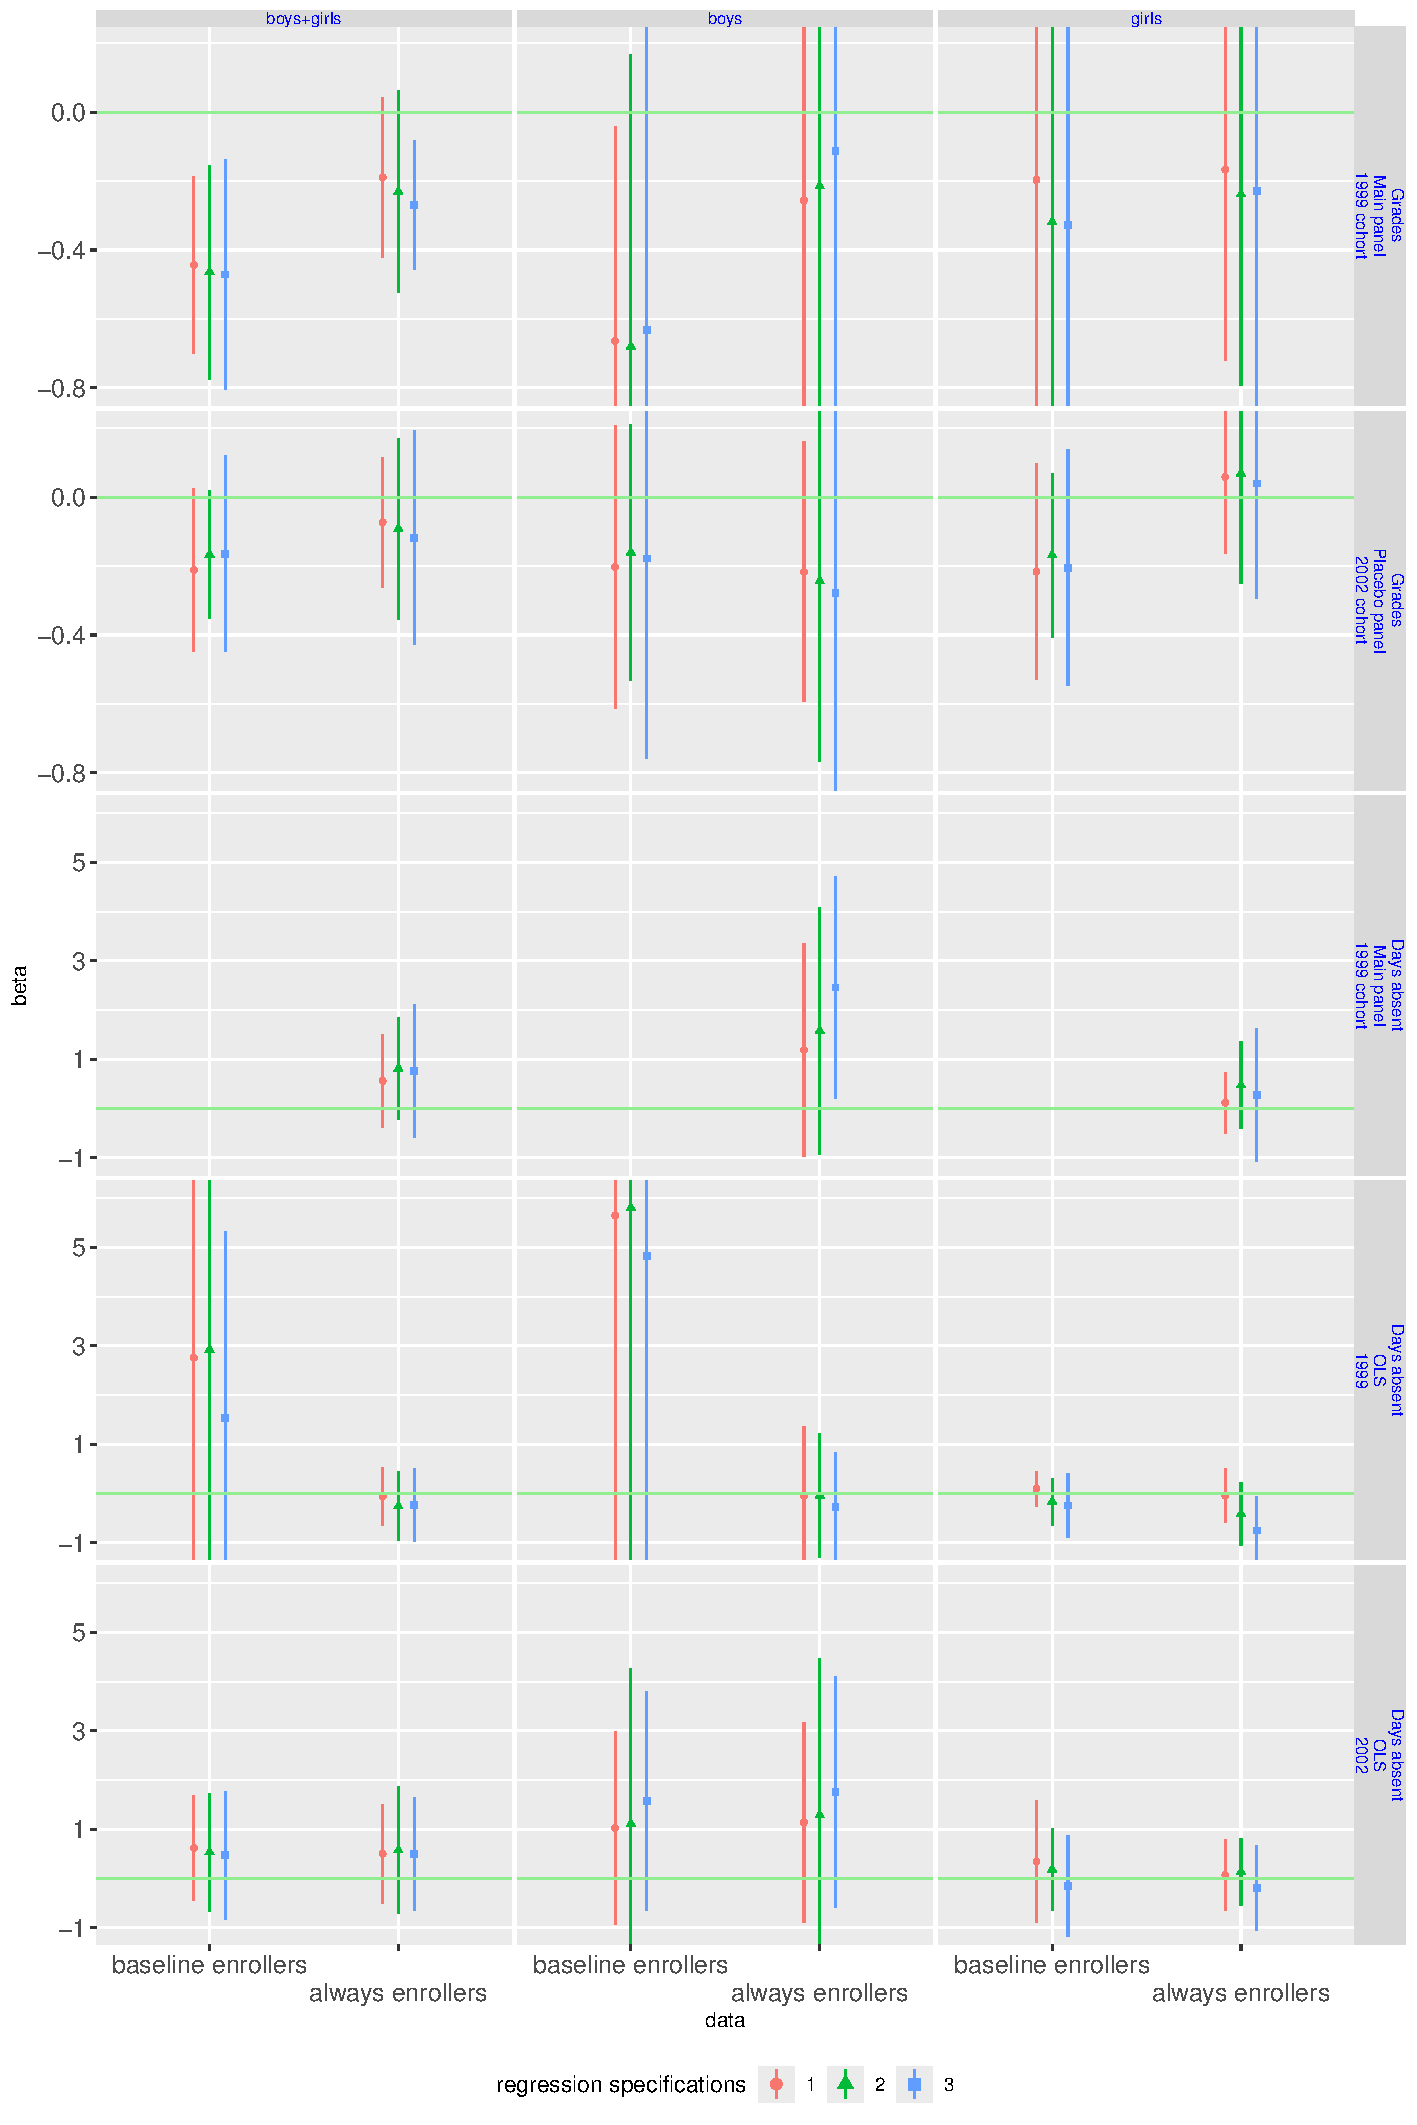
\includegraphics[width=.75\paperwidth]{../draft/Figures/App_NumGradesDaysAbsentPlotsByGender.pdf}\\
\renewcommand{\arraystretch}{1}
\hfil\begin{tabular}{>{\hfill\scriptsize}p{1cm}<{}>{\scriptsize}p{11cm}<{\hfill}}
Source: & Compiled from IFPRI data. \\[-1ex]
Notes:& 1. Grades: Number of grades, Days: Days absent. Days absent does not have placebo tests. The coefficients are dummies for agri-HH $\times$ year 2002.\\[-1ex]
& 2. Specifications 1 - 3 correspond to the same specifications in \textsc{Table \ref{base10}}. \\[-1ex]
& 3. Error bars are 95\% confidence intervals using standard errors clustered at thana level with a Satterthwaite correction for small number of clusters.
=======
\hfil 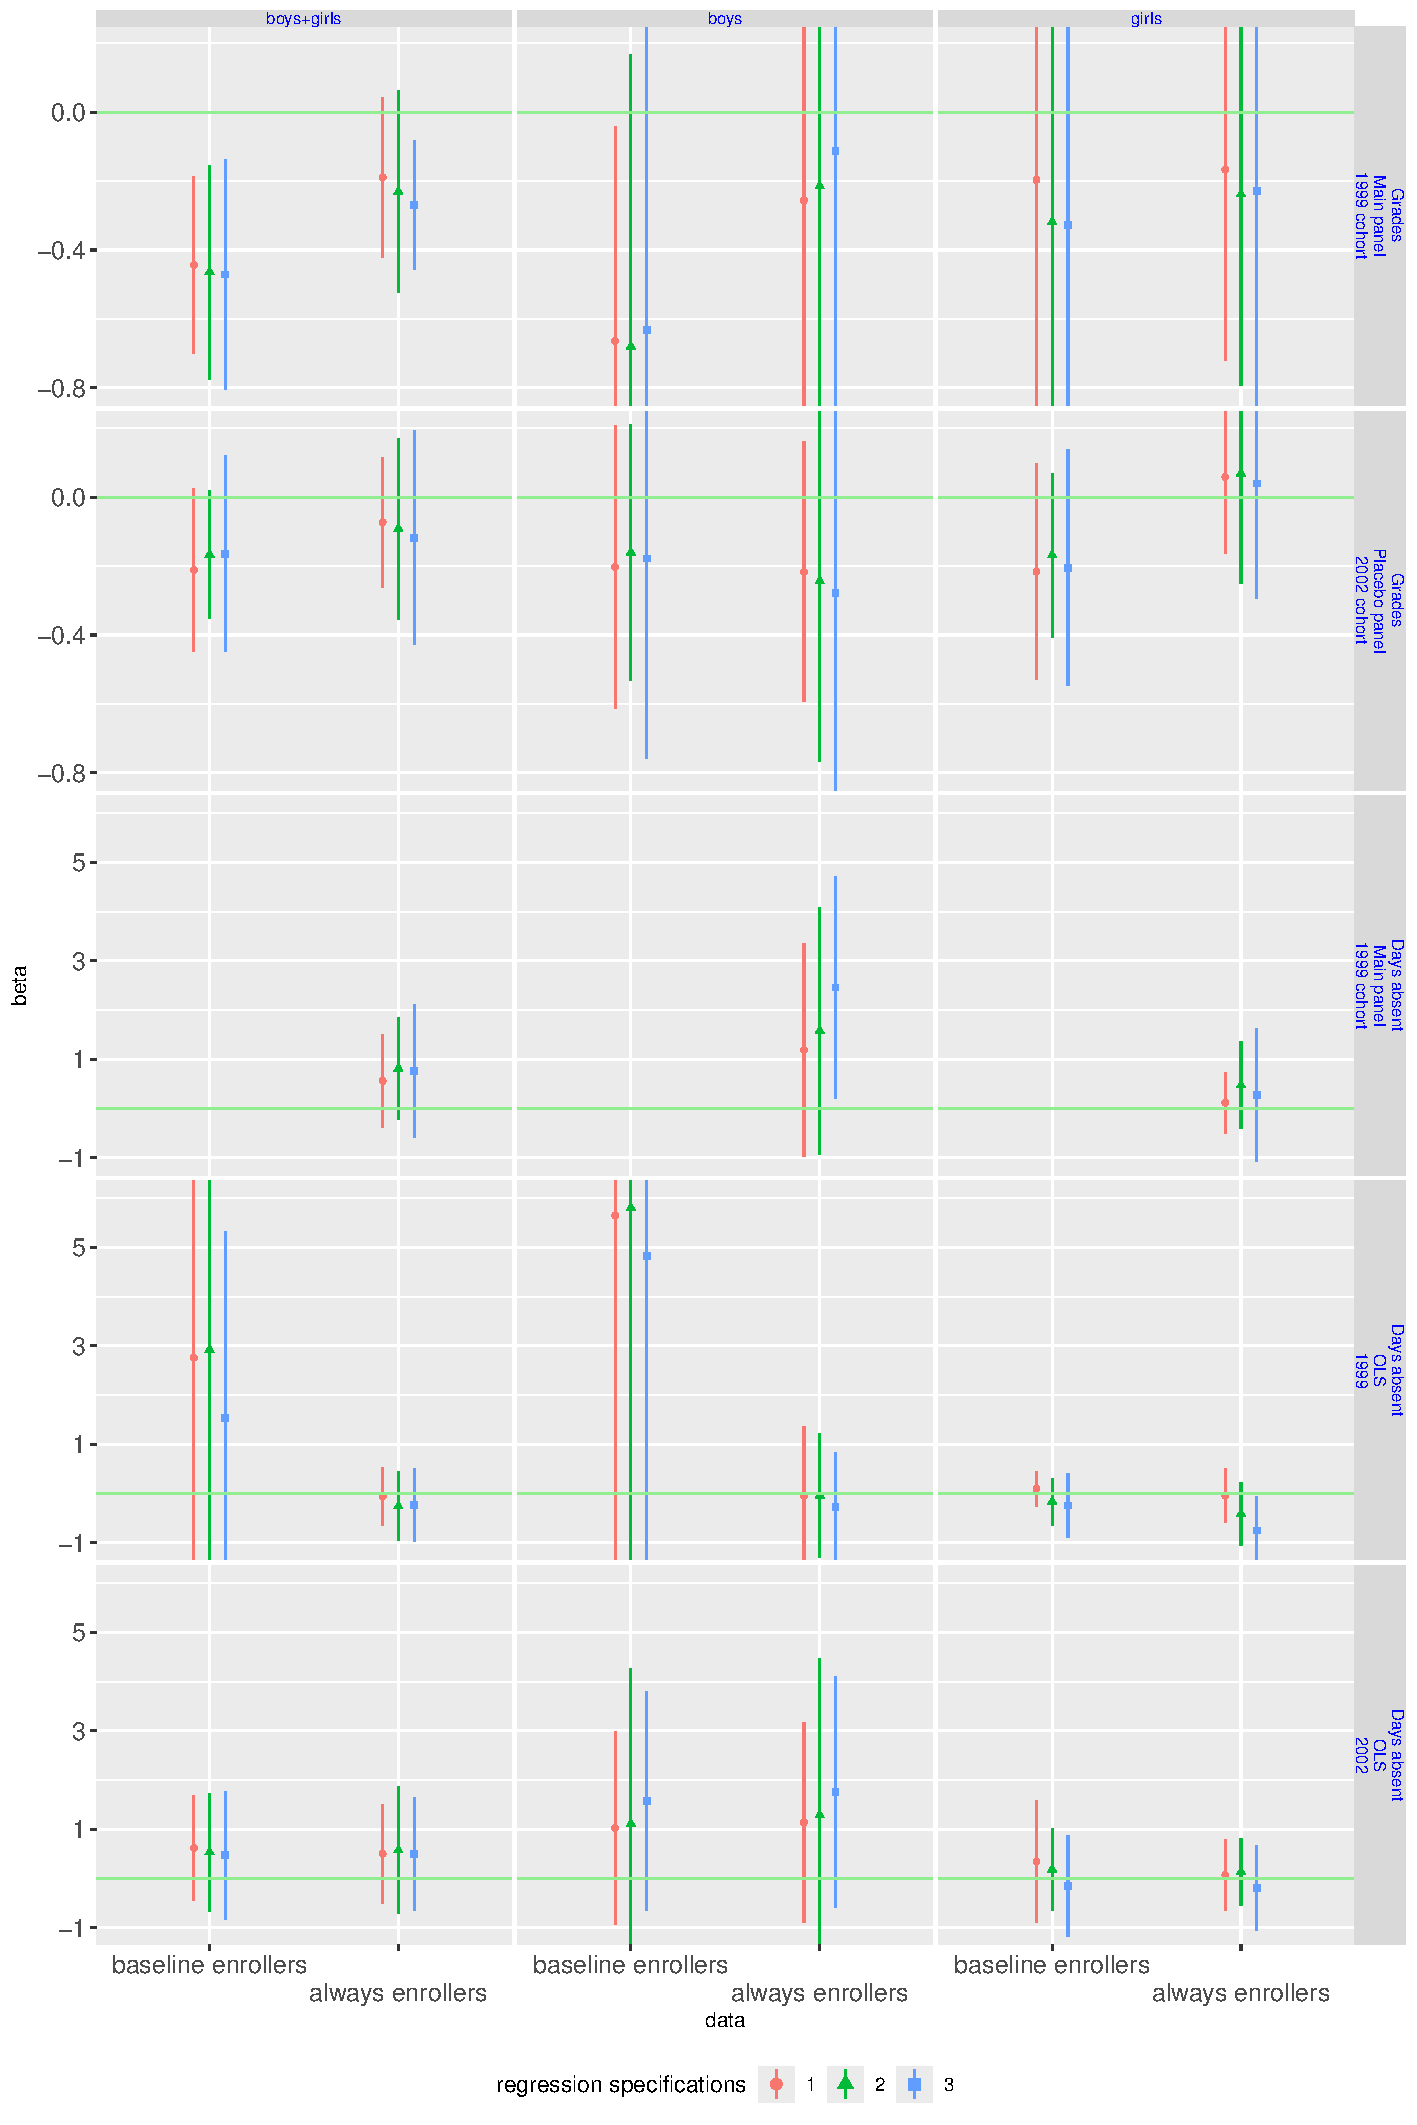
\includegraphics[height=.3\paperheight]{../draft/Figures/App_NumGradesDaysAbsentPlotsByGender.pdf}\\
\renewcommand{\arraystretch}{1}
\hfil\begin{tabular}{>{\hfill\scriptsize}p{1cm}<{}>{\hfill\scriptsize}p{.5cm}<{}>{\scriptsize}p{11cm}<{\hfill}}
Source: & \multicolumn{2}{l}{\scriptsize Compiled from IFPRI data.} \\[-1ex]
Notes:& 1. & Grades: Number of grades, Days: Days absent. Rows are for number of grades impacts, number of grades placebo impacts, and days absent impacts.  Panel of ``Days, placebo'' is not shown because there is no placebo test for it. Columns are for boys subsample, girls subsample, and full sample. \textsf{complete}: Complete panel sample, \textsf{incomplete}: Incomplete panel sample, \textsf{cross section 1999}: 1999 cross section estimate of incomplete panel sample, \textsf{cross section 2002}: 2002 cross section estimate of incomplete panel sample. The coefficients are for agricultural HH $\times$ year 2002 for ``Grades'', ``Days absent'' rows and agricultural HH $\times$ year 2006 for ``Grades, placebo'' row.\\[-1ex]
& 2. & Specifications 1 - 3 correspond to the same specifications in \textsc{Table \ref{base10}}. \\[-1ex]
& 3. & Error bars are 95\% confidence intervals using standard errors clustered at thana level with a Satterthwaite correction for small number of clusters.
>>>>>>> 41dec8f560b653fb2373d27136c157ebc2dfddbe
\end{tabular}
%\end{minipage}
\end{figure}

<<<<<<< HEAD
\begin{table}\hfil\textsc{\footnotesize Table \refstepcounter{table}\thetable: Other schooling outcomes, grade progression and days absent\label{zEm.1999.10.sameN}}\\\setlength{\tabcolsep}{.5pt}\renewcommand{\arraystretch}{.675}\hspace{-2em}\hfil\begin{tabular}{>{\scriptsize}p{3.25cm}<{\hfill}>{\hfil\scriptsize$}p{1.5cm}<{$}>{\hfil\scriptsize$}p{1.5cm}<{$}>{\hfil\scriptsize$}p{1.5cm}<{$}>{$}p{0.1cm}<{$}>{\hfil\scriptsize$}p{1.5cm}<{$}>{\hfil\scriptsize$}p{1.5cm}<{$}>{\hfil\scriptsize$}p{1.5cm}<{$}}
\hline
\makebox[3.25cm]{\scriptsize\hfil }&\multicolumn{3}{c}{\makebox[4.5cm]{\scriptsize \textsf{Grade progression}}}&&\multicolumn{3}{c}{\makebox[4.5cm]{\scriptsize \textsf{Days absent}}} \\[-.5ex]
\cline{2-4} \cline{6-8} \\[-1ex]
&\multicolumn{7}{c}{\scriptsize A. Students enrolled in 1999}\\
&(1)&(2)&(3)&&&&\\
\hspace{.5em}Agricultural HH & -0.443^{***} & -0.464^{**\phantom{*}} & -0.471^{**\phantom{*}} &  &  &  & \\[-1ex]
se$_{agHH.yr2}$ & (0.107)^{\phantom{**}} & (0.125)^{\phantom{**}} & (0.136)^{\phantom{**}} &  &  &  & \\[-1ex]
 & {0.5}^{\phantom{**}} & {1.1}^{\phantom{**}} & {1.4}^{\phantom{**}} &  &  &  & \\[-1ex]
 & \mbox{\tiny [-0.700, -0.186]} & \mbox{\tiny [-0.774, -0.153]} & \mbox{\tiny [-0.805, -0.137]} &  &  &  & \\[-1ex]
 &  & \mbox{\tiny [0.572, 1.430]} & \mbox{\tiny [0.647, 1.501]} &  &  &  & \\[-1ex]
 &  & \mbox{\tiny [0.531, 1.607]} & \mbox{\tiny [0.637, 1.775]} &  &  &  & \\
$\bar{R}^{2}$ & 0.0251 & 0.2614 & 0.2942 &  &  &  & \\
N: agHH &  & 210 &  &  &  &  & \\
N &  & 393 &  &  &  &  & \\
mean of control in 1999 &  & 5.1585 &  &  &  &  & \\
mean of treated in 1999 &  & 5.0476 &  &  &  &  & \\
mean of control in 2002 &  & 7.2732 &  &  &  &  & \\
mean of treated in 2002 &  & 6.7190 &  &  &  &  & \\
&\multicolumn{7}{c}{\scriptsize B. Students enrolled in 1999 and 2002}\\
&(4)&(5)&(6)&&(7)&(8)&(9)\\
\hspace{.5em}Agricultural HH & -0.189^{*\phantom{**}} & -0.231^{\phantom{***}} & -0.269^{**\phantom{*}} &  & 0.562^{\phantom{***}} & 0.815^{\phantom{***}} & 0.766^{\phantom{***}}\\[-1ex]
se$_{agHH.yr2}$ & (0.097)^{\phantom{**}} & (0.119)^{\phantom{**}} & (0.077)^{\phantom{**}} &  & (0.396)^{\phantom{**}} & (0.423)^{\phantom{**}} & (0.553)^{\phantom{**}}\\[-1ex]
 & {9.6}^{\phantom{**}} & {10.2}^{\phantom{**}} & {1.3}^{\phantom{**}} &  & {20.3}^{\phantom{**}} & {10.3}^{\phantom{**}} & {21.5}^{\phantom{**}}\\[-1ex]
 & \mbox{\tiny [-0.422, 0.044]} & \mbox{\tiny [-0.523, 0.062]} & \mbox{\tiny [-0.456, -0.081]} &  & \mbox{\tiny [-0.391, 1.515]} & \mbox{\tiny [-0.226, 1.857]} & \mbox{\tiny [-0.584, 2.116]}\\[-1ex]
 &  & \mbox{\tiny [0.161, 1.232]} & \mbox{\tiny [0.388, 1.320]} &  &  & \mbox{\tiny [-1.721, 0.824]} & \mbox{\tiny [-2.348, 0.088]}\\[-1ex]
 &  & \mbox{\tiny [0.419, 1.595]} & \mbox{\tiny [0.603, 1.738]} &  &  & \mbox{\tiny [-2.102, 2.695]} & \mbox{\tiny [-2.806, 1.596]}\\
$\bar{R}^{2}$ & 0.0064 & 0.2146 & 0.2565 &  & 0.0042 & 0.0665 & 0.1447\\
N: agHH &  & 126 &  &  &  & 129 & \\
N &  & 260 &  &  &  & 263 & \\
mean of control in 1999 &  & 4.9776 &  &  &  & 3.4030 & \\
mean of treated in 1999 &  & 4.7381 &  &  &  & 3.3437 & \\
mean of control in 2002 &  & 7.3731 &  &  &  & 3.0672 & \\
mean of treated in 2002 &  & 6.9444 &  &  &  & 3.5698 & \\
&\multicolumn{7}{c}{\scriptsize C. Students enrolled in 1999 and 2002, cross section OLS of 2000}\\
&&&&&(10)&(11)&(12)\\
Agricultural HH &  &  &  &  & -0.059^{\phantom{***}} & -0.258^{\phantom{***}} & -0.234^{\phantom{***}}\\[-1ex]
se$_{agHH}$ &  &  &  &  & (0.245)^{\phantom{**}} & (0.287)^{\phantom{**}} & (0.302)^{\phantom{**}}\\[-1ex]
 &  &  &  &  & {81.6}^{\phantom{**}} & {40.4}^{\phantom{**}} & {46.9}^{\phantom{**}}\\[-1ex]
 &  &  &  &  & \mbox{\tiny [-0.647, 0.529]} & \mbox{\tiny [-0.965, 0.448]} & \mbox{\tiny [-0.977, 0.510]}\\[-1ex]
 &  &  &  &  &  & \mbox{\tiny [-2.485, 0.861]} & \mbox{\tiny [-2.280, 0.796]}\\
$\bar{R}^{2}$ &  &  &  &  & 0.0001 & 0.0452 & 0.1814\\
N: agHH &  &  &  &  &  & 129 & \\
N &  &  &  &  &  & 263 & \\
mean of control in 1999 &  &  &  &  &  & 3.4030 & \\
mean of treated in 1999 &  &  &  &  &  & 3.3437 & \\
&\multicolumn{7}{c}{\scriptsize D. Students enrolled in 1999 and 2002, cross section OLS of 2003}\\
&&&&&(13)&(14)&(15)\\
Agricultural HH &  &  &  &  & 0.503^{\phantom{***}} & 0.574^{\phantom{***}} & 0.495^{\phantom{***}}\\[-1ex]
se$_{agHH}$ &  &  &  &  & (0.419)^{\phantom{**}} & (0.524)^{\phantom{**}} & (0.469)^{\phantom{**}}\\[-1ex]
 &  &  &  &  & {27.2}^{\phantom{**}} & {31.6}^{\phantom{**}} & {33.2}^{\phantom{**}}\\[-1ex]
 &  &  &  &  & \mbox{\tiny [-0.504, 1.509]} & \mbox{\tiny [-0.714, 1.863]} & \mbox{\tiny [-0.654, 1.644]}\\[-1ex]
 &  &  &  &  &  & \mbox{\tiny [-1.866, 0.652]} & \mbox{\tiny [-2.260, 0.461]}\\
$\bar{R}^{2}$ &  &  &  &  & 0.0053 & 0.0593 & 0.1816\\
N: agHH &  &  &  &  &  & 129 & \\
N &  &  &  &  &  & 263 & \\
mean of control in 2002 &  &  &  &  &  & 3.0672 & \\
mean of treated in 2002 &  &  &  &  &  & 3.5698 & \\
\multicolumn{8}{l}{\scriptsize Common specifications}\\
\hspace{.5em}Covariates, thana trends &  &  & \mbox{Y} &  &  &  & \mbox{Y}\\
\hspace{.5em}HH trends &  &  & \mbox{Y} &  &  &  & \mbox{Y}\\
\hline
\end{tabular}
\\\renewcommand{\arraystretch}{1}\hfil\begin{tabular}{>{\hfill\scriptsize}p{1cm}<{}>{\scriptsize}p{12cm}<{\hfill}} Source:& Compiled from IFPRI data. \\[-1ex] Notes:&   \textsf{Agricultural HH + year 2002} is an interaction term of agricultural household dummy and year 2002 dummy. All interaction terms are demeaned. For each panel, first columns are raw DID. Second columns add time-varying thana level characteristics (yield, mean rainfall, mean high temperature, mean low temperature), individual level characteristics (age squared, recipient of a poverty program), and \textsf{Thana trends} that are interactions of year 2002 dummy with Thana fixed effects. Third columns add interactions of year 2002 dummy and individual level characterstics (sex of individual, household head's and spouse's education, number of older male/female siblings, per member land holding, per member non land asset holding, piped water access, structured toilet access) $\bfx_{i}r_{t}$, and triple interactions of year 2002 dummy, individual characteristics, and agricultural household dummy $\bfx_{i}r_{t}D_{i}$. Rows of $\underline{\phantom{mm}}*x$ show estimates of the triple interaction term of $x_{i}$, or $x_{i}r_{t}D_{i}$. Parental education variables are strongly collinear with agricultural household dummy and are used only in year 2002 interaction terms to avoid multicollinearity., \\   \end{tabular} \end{table}
=======
\begin{table}\hfil\textsc{\footnotesize Table \refstepcounter{table}\thetable: Other schooling outcomes, grade progression and days absent\label{zEm.1999.10.sameN}}\\\setlength{\tabcolsep}{.5pt}\renewcommand{\arraystretch}{.675}\hspace{-2em}\hfil\begin{tabular}{>{\scriptsize}p{3.25cm}<{\hfill}>{\hfil\scriptsize$}p{1.5cm}<{$}>{\hfil\scriptsize$}p{1.5cm}<{$}>{\hfil\scriptsize$}p{1.5cm}<{$}>{$}p{0.1cm}<{$}>{\hfil\scriptsize$}p{1.5cm}<{$}>{\hfil\scriptsize$}p{1.5cm}<{$}>{\hfil\scriptsize$}p{1.5cm}<{$}}
\hline
\makebox[3.25cm]{\scriptsize\hfil }&\multicolumn{3}{c}{\makebox[4.5cm]{\scriptsize \textsf{Grade progression}}}&&\multicolumn{3}{c}{\makebox[4.5cm]{\scriptsize \textsf{Days absent}}} \\[-.5ex]
\cline{2-4} \cline{6-8} \\[-1ex]
&\multicolumn{7}{c}{\scriptsize A. Students enrolled in 1999}\\
&(1)&(2)&(3)&&&&\\
\hspace{.5em}Agricultural HH & -0.443^{***} & -0.464^{**\phantom{*}} & -0.471^{**\phantom{*}} &  &  &  & \\[-1ex]
se$_{agHH.yr2}$ & (0.107)^{\phantom{**}} & (0.125)^{\phantom{**}} & (0.136)^{\phantom{**}} &  &  &  & \\[-1ex]
 & {0.5}^{\phantom{**}} & {1.1}^{\phantom{**}} & {1.4}^{\phantom{**}} &  &  &  & \\[-1ex]
 & \mbox{\tiny [-0.700, -0.186]} & \mbox{\tiny [-0.774, -0.153]} & \mbox{\tiny [-0.805, -0.137]} &  &  &  & \\[-1ex]
 &  & \mbox{\tiny [0.572, 1.430]} & \mbox{\tiny [0.647, 1.501]} &  &  &  & \\[-1ex]
 &  & \mbox{\tiny [0.531, 1.607]} & \mbox{\tiny [0.637, 1.775]} &  &  &  & \\
$\bar{R}^{2}$ & 0.0251 & 0.2614 & 0.2942 &  &  &  & \\
N: agHH &  & 210 &  &  &  &  & \\
N &  & 393 &  &  &  &  & \\
mean of control in 1999 &  & 5.1585 &  &  &  &  & \\
mean of treated in 1999 &  & 5.0476 &  &  &  &  & \\
mean of control in 2002 &  & 7.2732 &  &  &  &  & \\
mean of treated in 2002 &  & 6.7190 &  &  &  &  & \\
&\multicolumn{7}{c}{\scriptsize B. Students enrolled in 1999 and 2002}\\
&(4)&(5)&(6)&&(7)&(8)&(9)\\
\hspace{.5em}Agricultural HH & -0.189^{*\phantom{**}} & -0.231^{\phantom{***}} & -0.269^{**\phantom{*}} &  & 0.562^{\phantom{***}} & 0.815^{\phantom{***}} & 0.766^{\phantom{***}}\\[-1ex]
se$_{agHH.yr2}$ & (0.097)^{\phantom{**}} & (0.119)^{\phantom{**}} & (0.077)^{\phantom{**}} &  & (0.396)^{\phantom{**}} & (0.423)^{\phantom{**}} & (0.553)^{\phantom{**}}\\[-1ex]
 & {9.6}^{\phantom{**}} & {10.2}^{\phantom{**}} & {1.3}^{\phantom{**}} &  & {20.3}^{\phantom{**}} & {10.3}^{\phantom{**}} & {21.5}^{\phantom{**}}\\[-1ex]
 & \mbox{\tiny [-0.422, 0.044]} & \mbox{\tiny [-0.523, 0.062]} & \mbox{\tiny [-0.456, -0.081]} &  & \mbox{\tiny [-0.391, 1.515]} & \mbox{\tiny [-0.226, 1.857]} & \mbox{\tiny [-0.584, 2.116]}\\[-1ex]
 &  & \mbox{\tiny [0.161, 1.232]} & \mbox{\tiny [0.388, 1.320]} &  &  & \mbox{\tiny [-1.721, 0.824]} & \mbox{\tiny [-2.348, 0.088]}\\[-1ex]
 &  & \mbox{\tiny [0.419, 1.595]} & \mbox{\tiny [0.603, 1.738]} &  &  & \mbox{\tiny [-2.102, 2.695]} & \mbox{\tiny [-2.806, 1.596]}\\
$\bar{R}^{2}$ & 0.0064 & 0.2146 & 0.2565 &  & 0.0042 & 0.0665 & 0.1447\\
N: agHH &  & 126 &  &  &  & 129 & \\
N &  & 260 &  &  &  & 263 & \\
mean of control in 1999 &  & 4.9776 &  &  &  & 3.4030 & \\
mean of treated in 1999 &  & 4.7381 &  &  &  & 3.3437 & \\
mean of control in 2002 &  & 7.3731 &  &  &  & 3.0672 & \\
mean of treated in 2002 &  & 6.9444 &  &  &  & 3.5698 & \\
&\multicolumn{7}{c}{\scriptsize C. Students enrolled in 1999 and 2002, cross section OLS of 2000}\\
&&&&&(10)&(11)&(12)\\
Agricultural HH &  &  &  &  & -0.059^{\phantom{***}} & -0.258^{\phantom{***}} & -0.234^{\phantom{***}}\\[-1ex]
se$_{agHH}$ &  &  &  &  & (0.245)^{\phantom{**}} & (0.287)^{\phantom{**}} & (0.302)^{\phantom{**}}\\[-1ex]
 &  &  &  &  & {81.6}^{\phantom{**}} & {40.4}^{\phantom{**}} & {46.9}^{\phantom{**}}\\[-1ex]
 &  &  &  &  & \mbox{\tiny [-0.647, 0.529]} & \mbox{\tiny [-0.965, 0.448]} & \mbox{\tiny [-0.977, 0.510]}\\[-1ex]
 &  &  &  &  &  & \mbox{\tiny [-2.485, 0.861]} & \mbox{\tiny [-2.280, 0.796]}\\
$\bar{R}^{2}$ &  &  &  &  & 0.0001 & 0.0452 & 0.1814\\
N: agHH &  &  &  &  &  & 129 & \\
N &  &  &  &  &  & 263 & \\
mean of control in 1999 &  &  &  &  &  & 3.4030 & \\
mean of treated in 1999 &  &  &  &  &  & 3.3437 & \\
&\multicolumn{7}{c}{\scriptsize D. Students enrolled in 1999 and 2002, cross section OLS of 2003}\\
&&&&&(13)&(14)&(15)\\
Agricultural HH &  &  &  &  & 0.503^{\phantom{***}} & 0.574^{\phantom{***}} & 0.495^{\phantom{***}}\\[-1ex]
se$_{agHH}$ &  &  &  &  & (0.419)^{\phantom{**}} & (0.524)^{\phantom{**}} & (0.469)^{\phantom{**}}\\[-1ex]
 &  &  &  &  & {27.2}^{\phantom{**}} & {31.6}^{\phantom{**}} & {33.2}^{\phantom{**}}\\[-1ex]
 &  &  &  &  & \mbox{\tiny [-0.504, 1.509]} & \mbox{\tiny [-0.714, 1.863]} & \mbox{\tiny [-0.654, 1.644]}\\[-1ex]
 &  &  &  &  &  & \mbox{\tiny [-1.866, 0.652]} & \mbox{\tiny [-2.260, 0.461]}\\
$\bar{R}^{2}$ &  &  &  &  & 0.0053 & 0.0593 & 0.1816\\
N: agHH &  &  &  &  &  & 129 & \\
N &  &  &  &  &  & 263 & \\
mean of control in 2002 &  &  &  &  &  & 3.0672 & \\
mean of treated in 2002 &  &  &  &  &  & 3.5698 & \\
\multicolumn{8}{l}{\scriptsize Common specifications}\\
\hspace{.5em}Covariates, thana trends &  &  & \mbox{Y} &  &  &  & \mbox{Y}\\
\hspace{.5em}HH trends &  &  & \mbox{Y} &  &  &  & \mbox{Y}\\
\hline
\end{tabular}
\\\renewcommand{\arraystretch}{1}\hfil\begin{tabular}{>{\hfill\scriptsize}p{1cm}<{}>{\scriptsize}p{12cm}<{\hfill}} Source:& Compiled from IFPRI data. \\[-1ex] Notes:&   \textsf{Agricultural HH * year 2002} is an interaction term of agricultural household dummy and year 2002 dummy. All interaction terms are demeaned. For each panel, first columns are raw DID. Second columns add time-varying thana level characteristics (yield, mean rainfall, mean high temperature, mean low temperature), individual level characteristics (age squared, recipient of a poverty program), and \textsf{Thana trends} that are interactions of year 2002 dummy with Thana fixed effects. Third columns add interactions of year 2002 dummy and individual level characterstics (sex of individual, household head's and spouse's education, number of older male/female siblings, per member land holding, per member non land asset holding, piped water access, structured toilet access) $\bfx_{i}r_{t}$, and triple interactions of year 2002 dummy, individual characteristics, and agricultural household dummy $\bfx_{i}r_{t}D_{i}$. Rows of $\underline{\phantom{mm}}*x$ show estimates of the triple interaction term of $x_{i}$, or $x_{i}r_{t}D_{i}$. Parental education variables are strongly collinear with agricultural household dummy and are used only in year 2002 interaction terms to avoid multicollinearity., \\   \end{tabular} \end{table}
>>>>>>> 41dec8f560b653fb2373d27136c157ebc2dfddbe


\clearpage
\subsection{Placebo}

%\begin{table}\hfil\textsc{\footnotesize Table \refstepcounter{table}\thetable: Placebo estimation 2002-2006\label{zEm.1999.10.sameN}}\\\setlength{\tabcolsep}{.5pt}\renewcommand{\arraystretch}{.675}\hspace{-2em}\hfil\input{../save/PlaceboOlder10ByGenderByAgHHdefResults1.tex}\\\renewcommand{\arraystretch}{1}\end{table}, \addtocounter{table}{-1}, \begin{table}\hfil\textsc{\footnotesize Table \refstepcounter{table}\thetable: Placebo estimation 2002-2006 (continued)\label{zEm.1999.10.sameN}}\\\setlength{\tabcolsep}{.5pt}\renewcommand{\arraystretch}{.675}\hspace{-3cm}\hfil\begin{tikzpicture}\node (tbl) {\input{../save/PlaceboOlder10ByGenderByAgHHdefResults2.tex}};\input{c:/data/ramadan/save/tablecolortemplate.tex}\end{tikzpicture}\\\renewcommand{\arraystretch}{1}\hfil\begin{tabular}{>{\hfill\scriptsize}p{1cm}<{}>{\scriptsize}p{12cm}<{\hfill}} Source:& Compiled from IFPRI data. \\[-1ex] Notes:&   \textsf{Agricultural HH * year 2002} is an interaction term of agricultural household dummy and year 2002 dummy. All interaction terms are demeaned. For each panel, first columns are raw DID. Second columns add time-varying thana level characteristics (yield, mean rainfall, mean high temperature, mean low temperature), individual level characteristics (age squared, recipient of a poverty program), and \textsf{Thana trends} that are interactions of year 2002 dummy with Thana fixed effects. Third columns add interactions of year 2002 dummy and individual level characterstics (sex of individual, household head's and spouse's education, number of older male/female siblings, per member land holding, per member non land asset holding, piped water access, structured toilet access) $\bfx_{i}r_{t}$, and triple interactions of year 2002 dummy, individual characteristics, and agricultural household dummy $\bfx_{i}r_{t}D_{i}$. Rows of $\underline{\phantom{mm}}*x$ show estimates of the triple interaction term of $x_{i}$, or $x_{i}r_{t}D_{i}$. Parental education variables are strongly collinear with agricultural household dummy and are used only in year 2002 interaction terms to avoid multicollinearity., \\   \end{tabular} \end{table}
%\addtocounter{table}{-1}
%\begin{table}\hfil\textsc{\footnotesize Table \refstepcounter{table}\thetable: Placebo estimation 2002-2006 (continued)\label{zEm.1999.10.sameN}}\\\setlength{\tabcolsep}{.5pt}\renewcommand{\arraystretch}{.675}\hspace{-2em}\hfil\input{../save/PlaceboOlder10ByGenderByAgHHdefResults3.tex}\\\renewcommand{\arraystretch}{1}\hfil\begin{tabular}{>{\hfill\scriptsize}p{1cm}<{}>{\scriptsize}p{12cm}<{\hfill}} Source:& Compiled from IFPRI data. \\[-1ex] Notes:&   \textsf{Agricultural HH * year 2002} is an interaction term of agricultural household dummy and year 2002 dummy. All interaction terms are demeaned. For each panel, first columns are raw DID. Second columns add time-varying thana level characteristics (yield, mean rainfall, mean high temperature, mean low temperature), individual level characteristics (age squared, recipient of a poverty program), and \textsf{Thana trends} that are interactions of year 2002 dummy with Thana fixed effects. Third columns add interactions of year 2002 dummy and individual level characterstics (sex of individual, household head's and spouse's education, number of older male/female siblings, per member land holding, per member non land asset holding, piped water access, structured toilet access) $\bfx_{i}r_{t}$, and triple interactions of year 2002 dummy, individual characteristics, and agricultural household dummy $\bfx_{i}r_{t}D_{i}$. Rows of $\underline{\phantom{mm}}*x$ show estimates of the triple interaction term of $x_{i}$, or $x_{i}r_{t}D_{i}$. Parental education variables are strongly collinear with agricultural household dummy and are used only in year 2002 interaction terms to avoid multicollinearity., \\   \end{tabular} \end{table}

\begin{Schunk}
\begin{Sinput}
lapply(tabfiles, subnums, num2, num1)
lapply(tabfiles, subnums, num4, num3)
lapply(tabfiles, subnums, num6, num5)
lapply(tabfiles, subnums, num8, num7)
\end{Sinput}
\end{Schunk}


\end{document}
